
\section{External Interface Requirements}
\label{sec:external_interface_requirements}

\subsection{User Interfaces}
\label{subsec:User_interfaces}

\begin{figure}[H]
    \begin{center}
        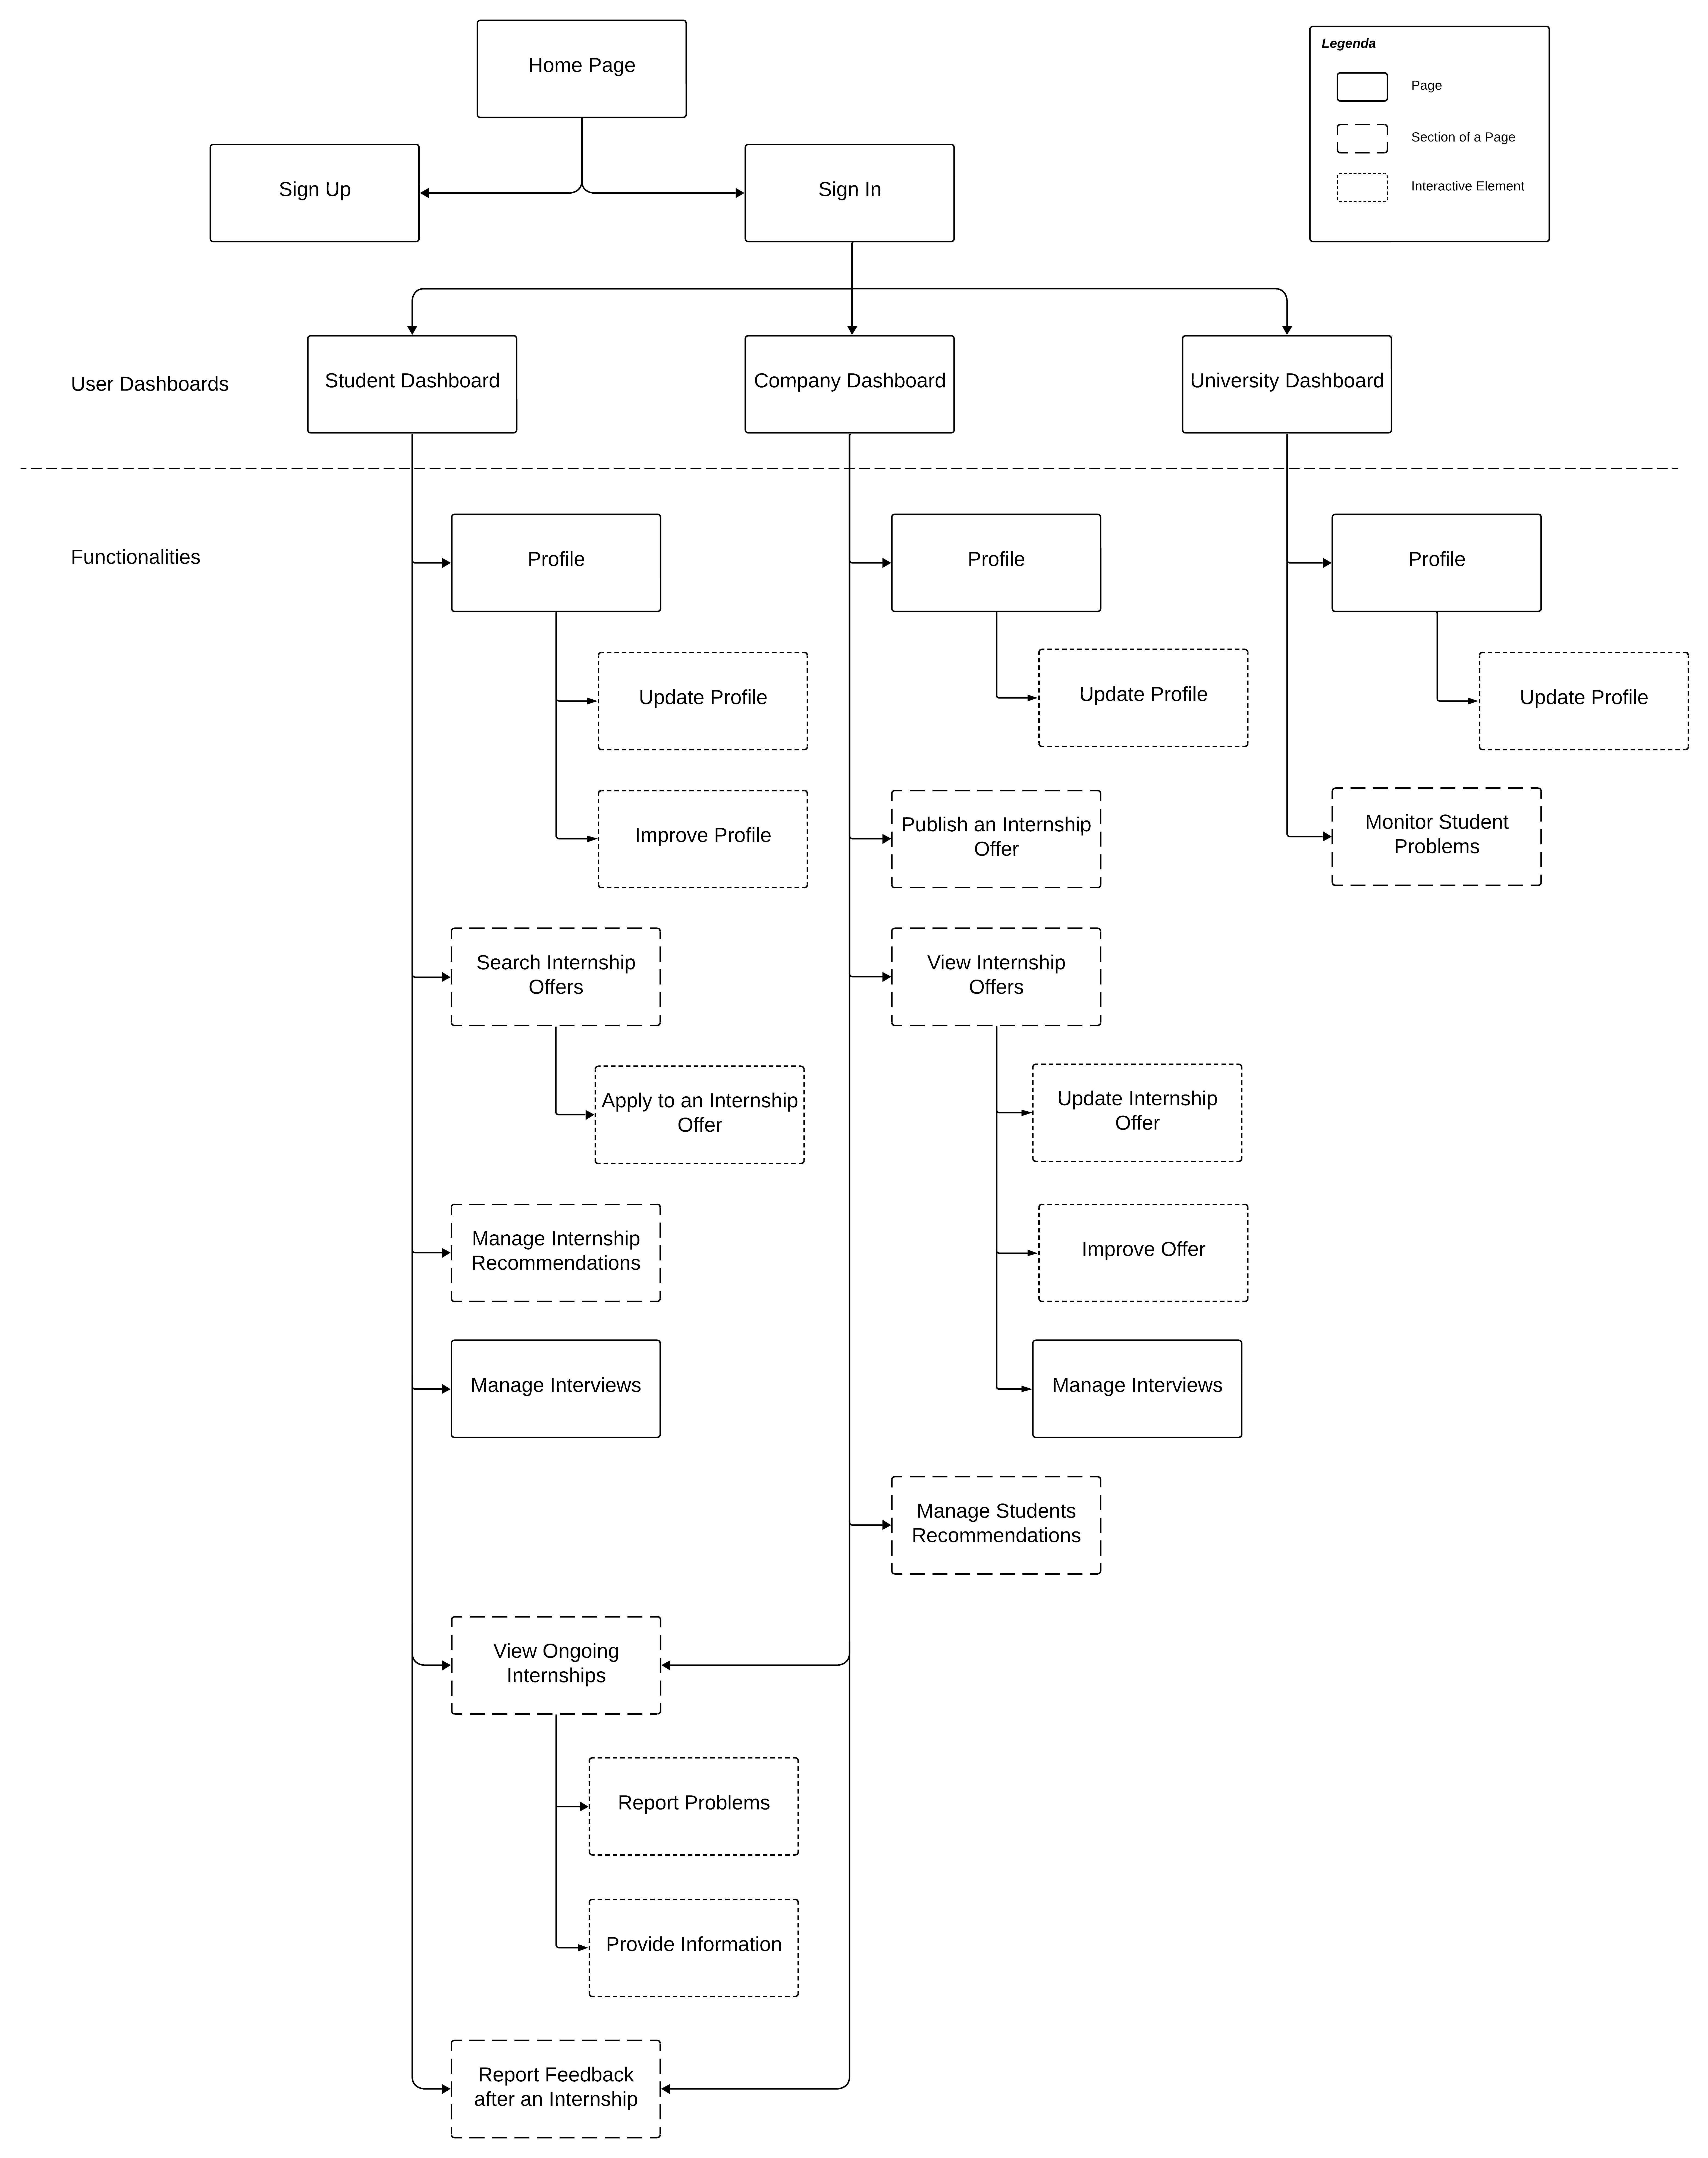
\includegraphics[width=0.7\linewidth]{LaTeXCode/images/webapp_map_workflow.png}
        \caption{WebApp Map} 
        \label{fig: webapp_map}
    \end{center}
\end{figure}

\newpage

The platform's user interface shall be designed to ensure usability and interactivity, adhering to web standards, briefly discussed in \hyperref[sec:standards_compliance]{\uline{3.4.1. Standards Compliance}}. The interface shall adapt responsively to various device displays, providing an intuitive layout and functionality across all the supported devices. Interface elements shall be organized in a layout that prioritizes clarity and ease of navigation for all the users.

Below is a description of the primary interfaces needed, as visually displayed in the above map, and how they should be grouped and structured:

\subparagraph{Home Page}
This page serves as the entry point to the platform and offers:
\begin{itemize}
    \item \textbf{Sign-Up (Register)}: A page to start the initial registration process for the three distinct user types.
    \item \textbf{Sign-In (Login)}: A page to perform login that redirects authenticated users to their respective dashboards.
\end{itemize}

\subparagraph{User Dashboards}
Each user type is provided with a personalized dashboard, divided into sections offering different functionalities:

\begin{enumerate}
    \item \textbf{Student Dashboard}
    \begin{itemize}
        \item \textbf{Search Internship Offers}: a section that includes a search bar with filtering options to search offers. Each result of the query is an interactive element displaying an overview of the information related to an internship offer; clicking on the internship offer expands its details and enables an interactive element to apply to it.
        \item \textbf{Manage Internship Recommendations}: a section listing the received internship recommendations. Each recommendation is an interactive element, and students can visualize details about the internship offer associated to each recommendation and accept, reject, or postpone the recommendations.
        \item \textbf{Manage Invitations}: a section displaying interview invitations. Each invitation is an interactive element, and Students can confirm or decline, providing a reason, based on their availability. Questions posted by companies are also made available in a parallel section as interactive elements and are displayed here.
        \item \textbf{Monitor Interviews}: a section displaying the status of interview processes. Each interview is an interactive element, and Students can visualize the status and outcome of each interview.
        \item \textbf{View Internships}: a section displaying all ongoing and past internships. Each internship is an interactive element and based on its status, it allows students to:
        \begin{itemize}
            \item \textbf{Report Problems}: an interactive element to report problems to be handled by the university.
            \item \textbf{Report Feedback after an Internship}: an interactive element to give feedback upon completion of an internship.
        \end{itemize}
        \item \textbf{Provide Information}: a section where to write relevant information during an internship and communicate with the other party.
        \item \textbf{Profile}: a page displaying all the student's information and including:
        \begin{itemize}
            \item \textbf{Update Profile}: an interactive element for updating personal and academic information.
            \item \textbf{Improve Profile}: an interactive element suggesting optimizations based on the content of the profile and CV.
        \end{itemize}
    \end{itemize}

    \item \textbf{Company Dashboard}
    \begin{itemize}      
        \item \textbf{Publish an Internship Offer}: an interactive element to publish new internship offers.
        \item \textbf{View Internship Offers}: a section listing all published internship offers. Each internship offer is an interactive element displaying an overview of the information related to an internship offer; clicking on the internship offer expands its details.
        Via interactive elements it allow the company to:
        \begin{itemize}
            \item \textbf{Update an Internship Offer}: an interactive element for updating the offer information.
            \item \textbf{Improve Offer}: an interactive element to receive optimizations based on the offer details.
            \item \textbf{Shortcut - Manage Interviews}: a shortcut allowing companies to handle interview invitations and post questions to candidates about a specific internship offer.
            \item \textbf{Shortcut - Manage Student Recommendations}: a shortcut allowing companies to manage students recommendations about a specific internship offer.
        \end{itemize}
        \item \textbf{Manage Student Recommendations}: a section listing student's recommendations. Each recommendation is an interactive element, and the company can visualize the profile of the recommended student and accept, reject, or postpone it.
        \item \textbf{Manage Invitations}: a section offering an interactive element to create and display interview invitations. Each invitation is an interactive element, and the company can monitor the status of each of them. Questions posted by companies are also made available in A parallel section allows companies to post new questions to candidates and visualize the answers provided by them to previously submitted questions.
        \item \textbf{Manage Interviews}: a section displaying the status of interview processes. Each interview is an interactive element, and companies can update their status, also finalizing the selection process, and provide a feedback when an interview is completed.
        \item \textbf{View Internships}: a section displaying all ongoing and past internships. Each internship is an interactive element and based on its status, it allows companies to:
        \begin{itemize}
            \item \textbf{Report Problems}: an interactive element to report problems to be handled by the university.
            \item \textbf{Report Feedback after an Internship}: an interactive element to give feedback upon completion of an internship.
        \end{itemize}
        \item \textbf{Provide Information}: a section where to write relevant information during an internship and communicate with the other party.
        \item \textbf{Profile}: a page displaying all the company's information and including:
        \begin{itemize}
            \item \textbf{Update Profile}: an interactive element for updating company information.
        \end{itemize}  
    \end{itemize}

    \item \textbf{University Dashboard}
    \begin{itemize}  
        \item \textbf{Monitor Student Problems}: a section displaying issues reported by students during internships. Each report is an interactive element and provides tools to review, resolve, and update statuses.
        \item \textbf{Profile}: a page displaying all university-related information and including:
        \begin{itemize}
            \item \textbf{Update Profile}: an interactive element for updating information.
        \end{itemize} 
    \end{itemize}
\end{enumerate}

\subsection{Software Interfaces}
\label{subsec:software_interfaces}

The system is meant to be a platform-independent WebApp, which does not rely on external APIs or essential third-party software to perform its core functionalities. 
However, the system shall adhere to the following requirements:

\begin{itemize}
    \item It shall function across the most widely adopted operating systems, including but not limited to Microsoft Windows, MacOSX, Linux, Android, iOS and ChromeOS.
    
    \item It shall function across the most widely used browsers, including, but not limited to, Google Chrome, Opera, Mozilla Firefox, Safari, and Microsoft Edge, without requiring additional software installation on the user’s device.

    \item It shall interact appropriately with the chosen services or network protocols for email management, in order to carry on sign-up and sign-in functionalities.
\end{itemize}

No additional software installations or configurations are required on the user's device beyond the availability of a supported web browser.

\subsection{Communication Interfaces}
\label{subsec:communication_interfaces}

The system shall support standard communication protocols for reliable interaction between the components. Specifically, the following requirements apply:

\begin{itemize}
    \item The system shall operate over standard internet connections, including wired and wireless networks (e.g. Ethernet, Wi-Fi, mobile data).

    \item The system shall support encrypted communication/secure sessions (e.g. through TLS/SSL) to protect sensitive data, including user credentials and personal information, during transmission.

    \item The system shall utilize a widely adopted web communication protocol (such as HTTPS) to ensure secure and reliable data transmission between the user's browser and the web server.

    \item The system shall not require users to install additional software to facilitate communication.

    \item The system shall minimize communication latency to provide a responsive user experience, with server response times aligning with industry standards for web applications.
\end{itemize}

\subsection{Hardware Interfaces}
\label{subsec:hardware_interfaces}

The system shall ensure compatibility with common user devices and hosting infrastructure, designed to provide performance and accessibility.

\subsubsection{User Devices}

The platform shall support access from a wide range of devices commonly used by end-users, including but not limited to: desktop and laptop computers, tablets and smartphones.

The platform shall ensure responsiveness and usability across different device types and display resolutions, requiring hardware with free space for caching that can run modern web applications efficiently.

\subsubsection{Hosting Infrastructure}

The system shall be deployed on an infrastructure capable of supporting:

\begin{itemize}
    \item Simultaneous access by multiple users with minimal latency
    \item Data processing and storage necessary for handling user interactions and background operations
\end{itemize}

The hosting environment shall be scalable to accommodate growth in usage and computational demands while maintaining reliable service availability.

\section{Functional Requirements}
\label{sec:functional_requirements}

\begin{figure}[H]
    \begin{center}
        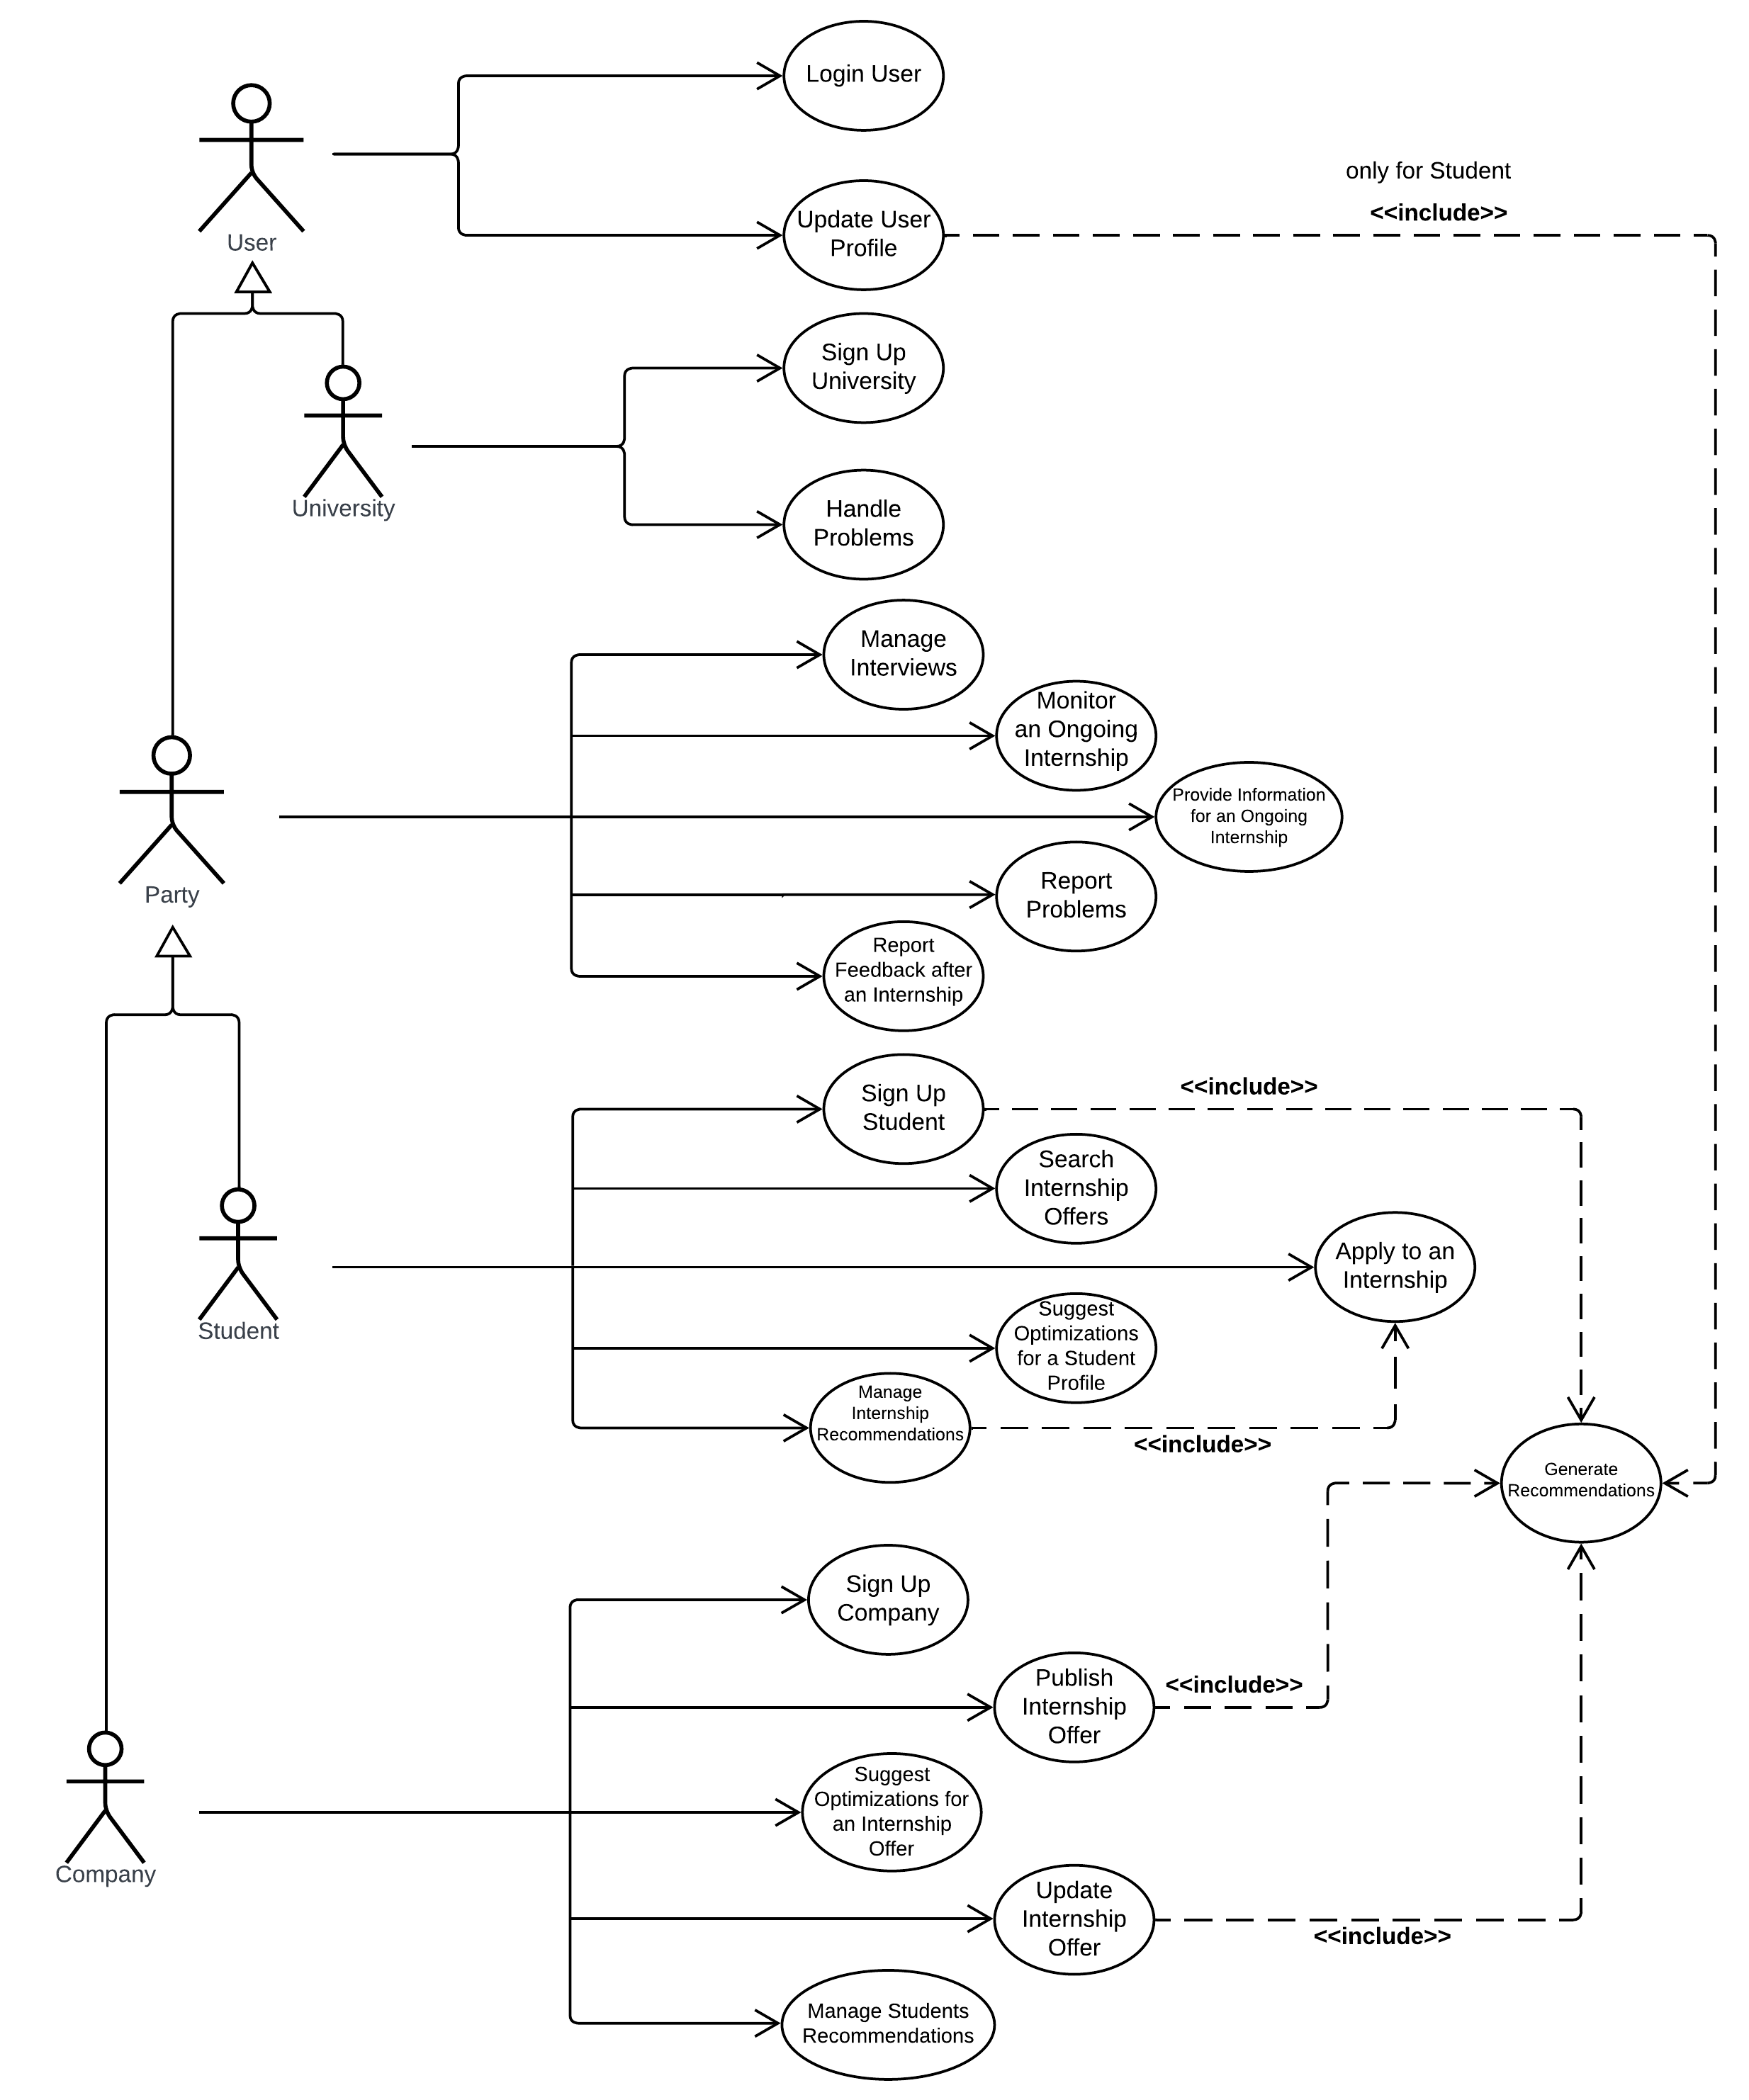
\includegraphics[width=0.9\linewidth]{LaTeXCode/images/Use Case Diagram of S&C.png}
        \caption{Use Case Diagram} 
        \label{fig:use_case_diagram}
    \end{center}
\end{figure}

\newpage
\subsection{Use Cases and Activity Diagrams}
\label{subsec: use_cases}%

\newcounter{ucsteps}
\setcounter{ucsteps}{1}
\newcommand{\cucsteps}{\theucsteps\stepcounter{ucsteps}}
\newcommand{\resetucsteps}{\setcounter{ucsteps}{1}}

\newcounter{uc}
\setcounter{uc}{1}
\newcommand{\cuc}{\theuc\stepcounter{uc}\resetucsteps}

\subsubsection*{UC\cuc . Sign Up by a Student}
\begin{center}
    \begin{longtable}{|l|p{0.75\linewidth}|}
        \hline
        \textbf{Actor}            & Student\\
        \hline
        \textbf{Entry Conditions} & The Student is not logged into the S\&C platform. \\
        \hline
        \textbf{Flow of Events}    
        & \cucsteps. On the homepage, the Student clicks the "Sign Up" button, entering the initial registration page. \\
        & \cucsteps. The Student provides the required details: User category (Student), email, password and password confirmation. \\
        & \cucsteps. The Student confirms the provided information by clicking the "Register" button. \\
        & \cucsteps. The system sends to the indicated mailbox a confirmation email with a link that expires in 24 hours for account verification purposes. \\
        & \cucsteps. The Student clicks the link in the confirmation email before it expires and logs into the platform. \\
        & \cucsteps. On the profile page, the Student completes their profile by inserting:
        name, surname, date of birth, gender, compiling its CV, selecting their university from a drop-down list and adding relevant details: skills, education, and career aspirations. \\
        & \cucsteps. The system starts an instance of the process for identifying new recommendations via the \hyperref[subsec: generate_recommendations_uc]{\uline{UC. Generate Recommendations}} functionality. \\
        \hline
        \textbf{Exit Conditions}   & The profile is complete and the Student has access to its functionalities.\\       
        \hline
        \textbf{Exceptions}       & \begin{itemize}
            \item The email address is already linked to an existing account: an error message is shown, and the Student is redirected to the login page.
            \item The password does not meet the platform's security requirements: an error message is displayed, and the Student is prompted to correct the password.
            \item Some mandatory fields are missing: the system doesn't allow the Student to complete the procedure until all the mandatory fields are filled out.
            \item The confirmation link sent to the indicated mailbox expires: all the information previously inserted into the system by the Student is discarded, and the link is invalidated.
        \end{itemize} \\
        \hline
    \end{longtable}
\end{center}

\begin{figure}[H]
    \begin{center}
         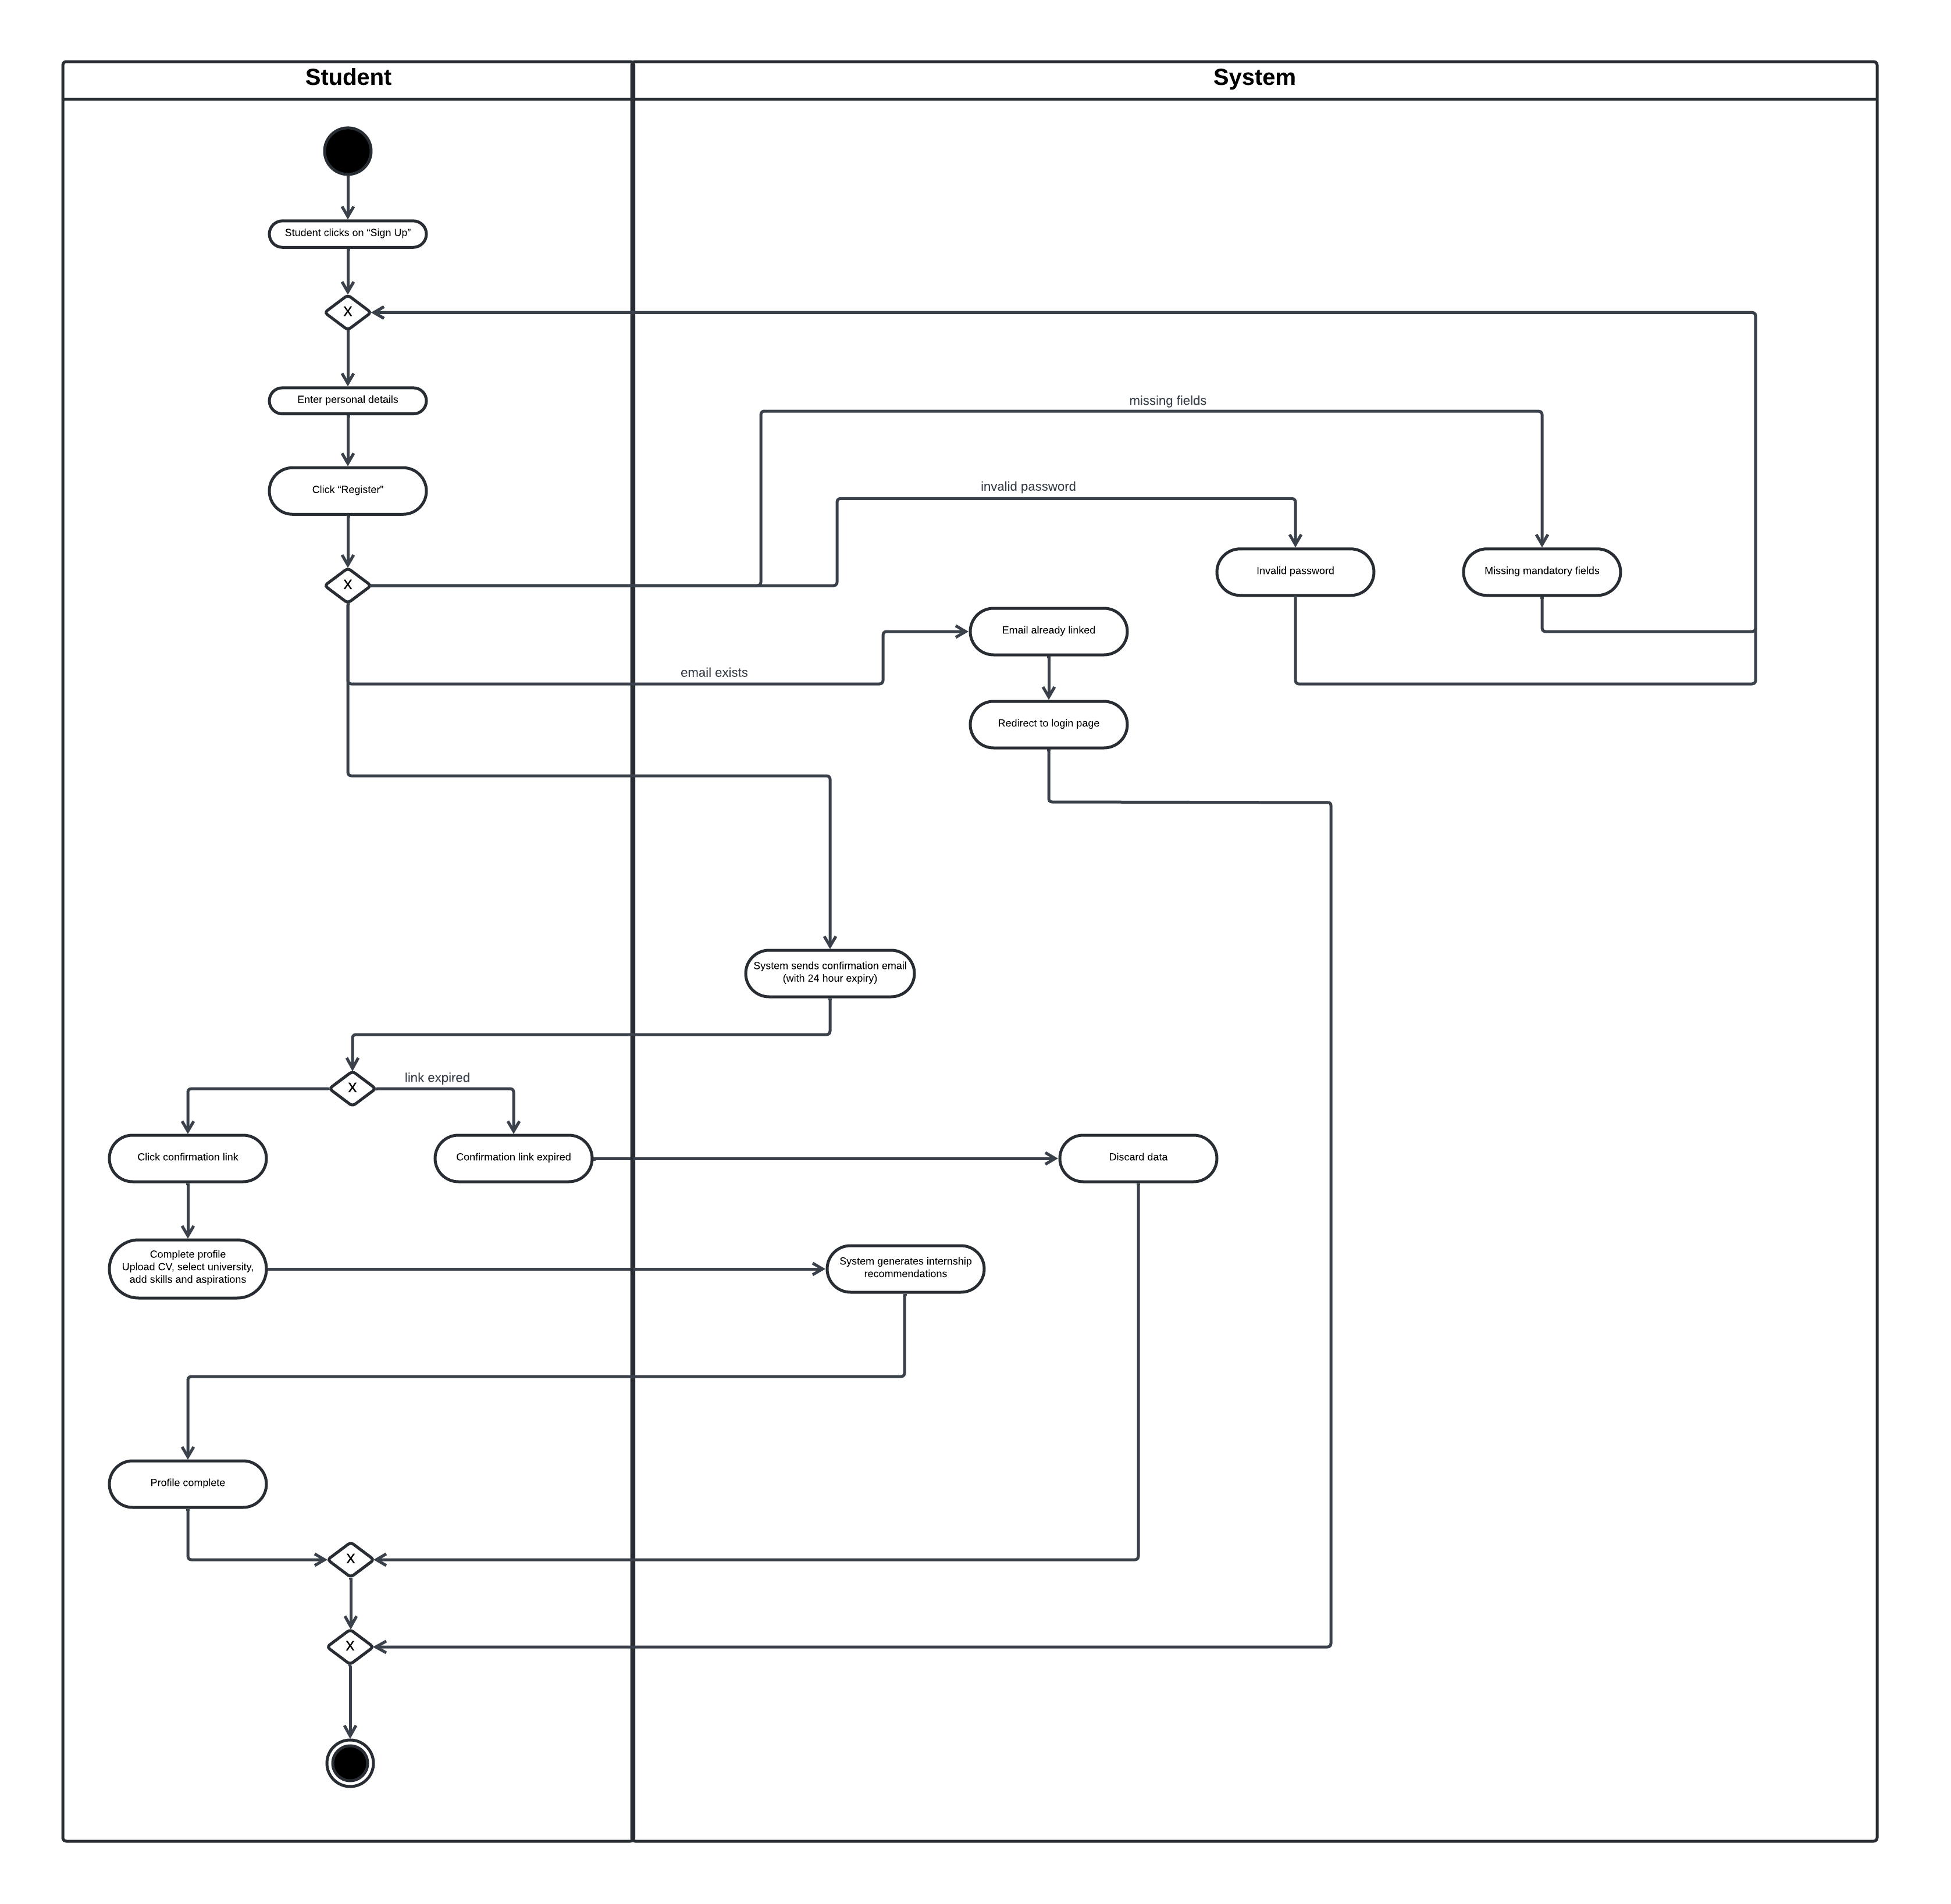
\includegraphics[width=1\linewidth]{LaTeXCode/images/activity diagram/UC1.png}
         \caption{Sign Up by a Student}
         \label{fig:signup_student_ad}
     \end{center}
\end{figure}

\newpage

\subsubsection*{UC\cuc . Sign Up by a Company}
\begin{center}
    \begin{longtable}{|l|p{0.75\linewidth}|}
        \hline
        \textbf{Actor}            & Company \\
        \hline
        \textbf{Entry Conditions} & The Company is not logged into the S\&C platform. \\
        \hline
        \textbf{Flow of Events}       
        & \cucsteps. On the homepage, the Company clicks the "Sign Up" button, entering the companies' registration page. \\
        & \cucsteps. The Company provides the required details: User category (Company), email, password and password confirmation. \\
        & \cucsteps. The Company confirms the provided information by clicking the "Register" button. \\
        & \cucsteps. The system sends to the indicated mailbox a confirmation email with a link that expires in 24 hours for account verification purposes. \\
        & \cucsteps. The Company clicks the link in the confirmation email and logs into the platform. \\
        & \cucsteps. On the profile page, the Company completes the company's profile by adding all other information and relevant details: company name, location, phone number,
        company description, mission, vision, and field in which it operates, and uploading its logo. \\
        \hline
        \textbf{Exit Conditions}   & The profile is complete and the Company has access to all its functionalities. \\       
        \hline
        \textbf{Exceptions}       & \begin{itemize}
            \item The email address is already linked to an existing account: an error message is shown, and the Company is redirected to the login page.
            \item The password does not meet the platform security requirements: An error message is displayed, and the Company is prompted to correct the password.
            \item Some mandatory fields are missing: the system does not allow the Company to complete the procedure until all the mandatory fields are filled out.
            \item The confirmation link sent to the indicated mailbox expires: all information previously inserted into the system by the Company is discarded and the link is invalidated.
        \end{itemize}\\
        \hline
    \end{longtable}
\end{center}

\begin{figure}[H]
    \begin{center}
         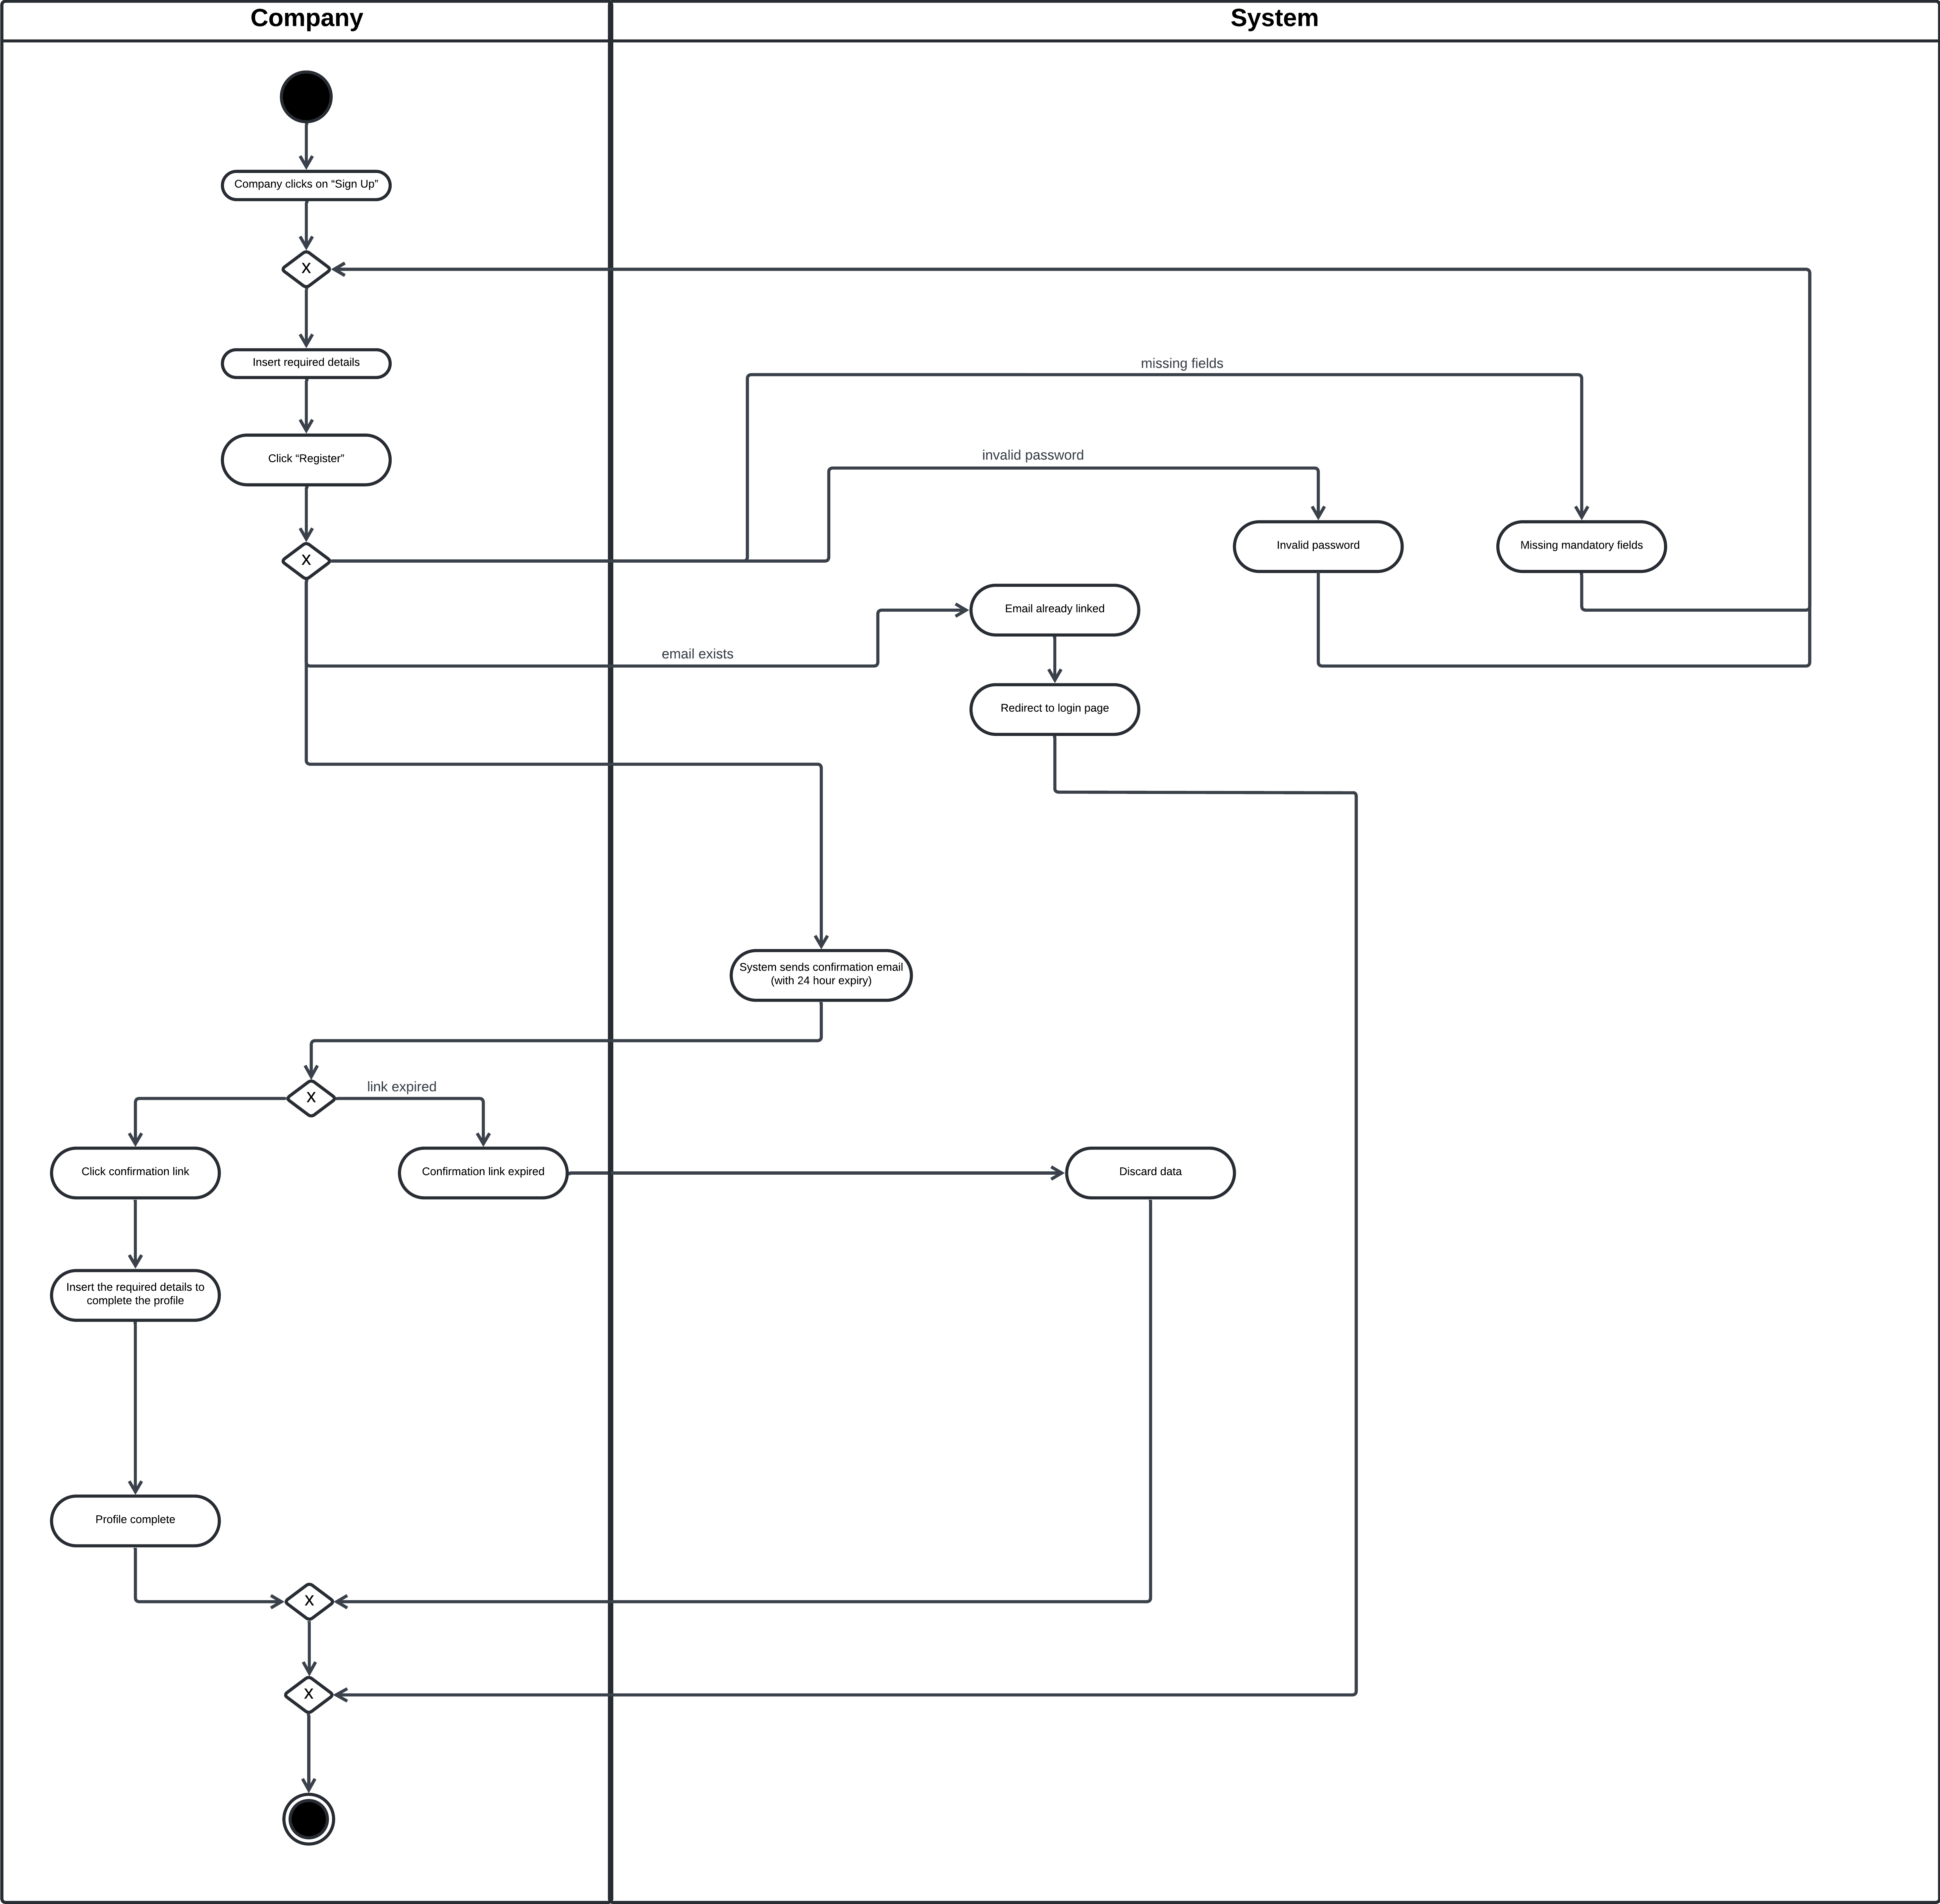
\includegraphics[width=1\linewidth]{LaTeXCode/images/activity diagram/UC2.png}
         \caption{Sign Up by a Company}
         \label{fig:signup_company_ad}
     \end{center}
\end{figure}

\newpage

\subsubsection*{UC\cuc . Sign Up by a University}
\begin{center}
    \begin{longtable}{|l|p{0.75\linewidth}|}
        \hline
        \textbf{Actor}            & University\\
        \hline
        \textbf{Entry Conditions} & The University is not logged into the S\&C platform. \\
        \hline
        \textbf{Flow of Events}       
        & \cucsteps. On the homepage, the University clicks the "Sign Up" button, entering the companies' registration page. \\
        & \cucsteps. The University provides the required details: User category (University), email, password and password confirmation. \\
        & \cucsteps. The University confirms the provided information by clicking the "Register" button. \\
        & \cucsteps. The system sends to the indicated mailbox a confirmation email with a link that expires in 24 hours for account verification purposes. \\
        & \cucsteps. The University clicks the link in the confirmation email and logs into the platform. \\
        & \cucsteps. On the profile page, the University completes the university's profile by adding relevant details: university name, location, phone number, faculties, key contacts for internships, university website. \\
        \hline
        \textbf{Exit Conditions}   & The profile is complete and the University has access to all its functionalities. \\       
        \hline
        \textbf{Exceptions}       & \begin{itemize}
            \item The email address is already linked to an existing account: an error message is shown, and the University is redirected to the login page.
            \item The password does not meet the platform security requirements: An error message is displayed, and the University is required to correct the password.
            \item Some mandatory fields are missing: the system does not allow the University to complete the procedure until all the mandatory fields are filled out.
            \item The confirmation link sent to the indicated mailbox expires: all information previously inserted into the system by the University is discarded and the link is invalidated.
        \end{itemize}\\
        \hline
    \end{longtable}
\end{center}

\begin{figure}[H]
    \begin{center}
         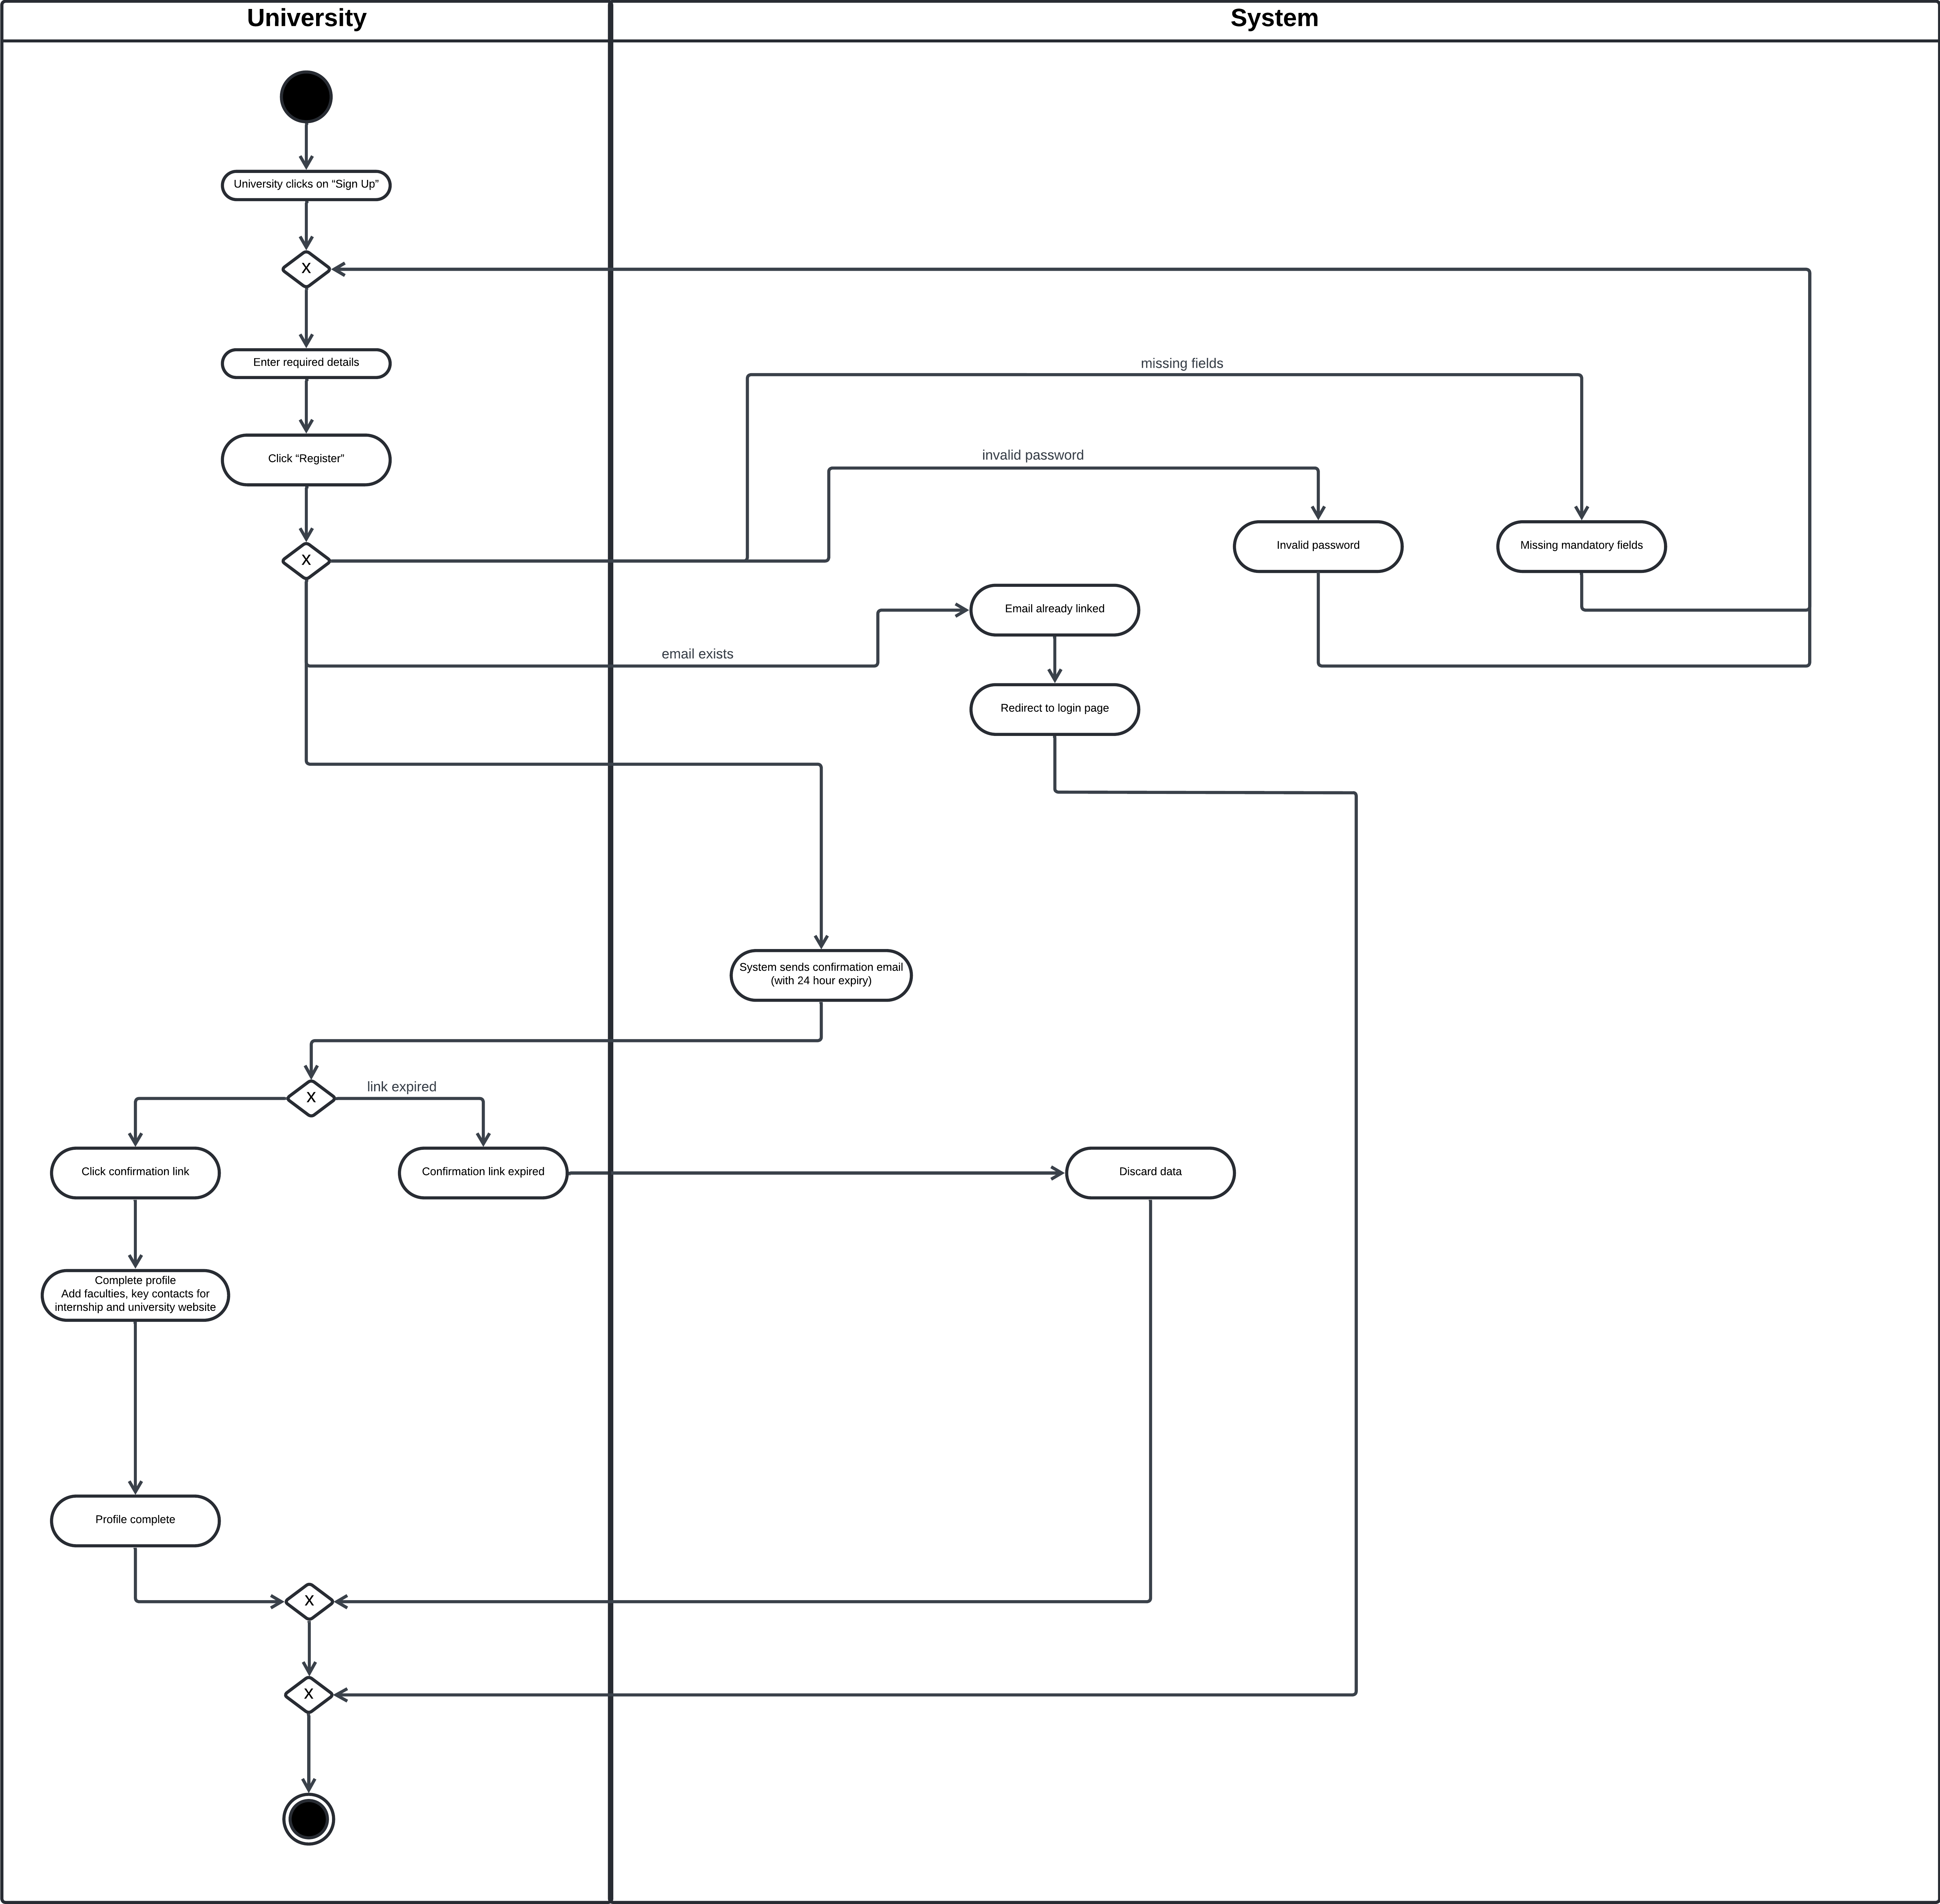
\includegraphics[width=1\linewidth]{LaTeXCode/images/activity diagram/UC3.png}
         \caption{Sign Up by a University}
         \label{fig:signup_university_ad}
     \end{center}
\end{figure}

\newpage

\subsubsection*{UC\cuc . Log In by a User}
\begin{center}
    \begin{longtable}{|l|p{0.75\linewidth}|}
        \hline
        \textbf{Actor}            & User (Student, Company or University) \\
        \hline
        \textbf{Entry Conditions} & The User is not already logged into the S\&C platform. \\
        \hline
        \textbf{Flow of Events}       
        & \cucsteps. On the homepage, the User clicks the "Login" button, which displays the login form. \\
        & \cucsteps. The User enters their email and password into the designated fields. \\
        & \cucsteps. The User clicks the "Login" button. \\
        & \cucsteps. The system validates the provided credentials. \\
        & \cucsteps. The system redirects the User to the dashboard page. \\
        \hline
        \textbf{Exit Conditions}   & The User is successfully logged in. \\       
        \hline
        \textbf{Exceptions}       & \begin{itemize}
            \item The inserted credentials are incorrect: the system displays an error message indicating that the credentials are invalid and the User remains on the login page.
            \item The account hasn't been verified yet: if the User has not confirmed their email and the confirmation link has not expired yet, the system shows a message requesting to complete the verification process.
            \item The profile of the logged User is incomplete: the User is redirected to the Update Profile page instead of the dashboard page.
        \end{itemize}\\
        \hline
    \end{longtable}
\end{center}

\begin{figure}[H]
    \begin{center}
         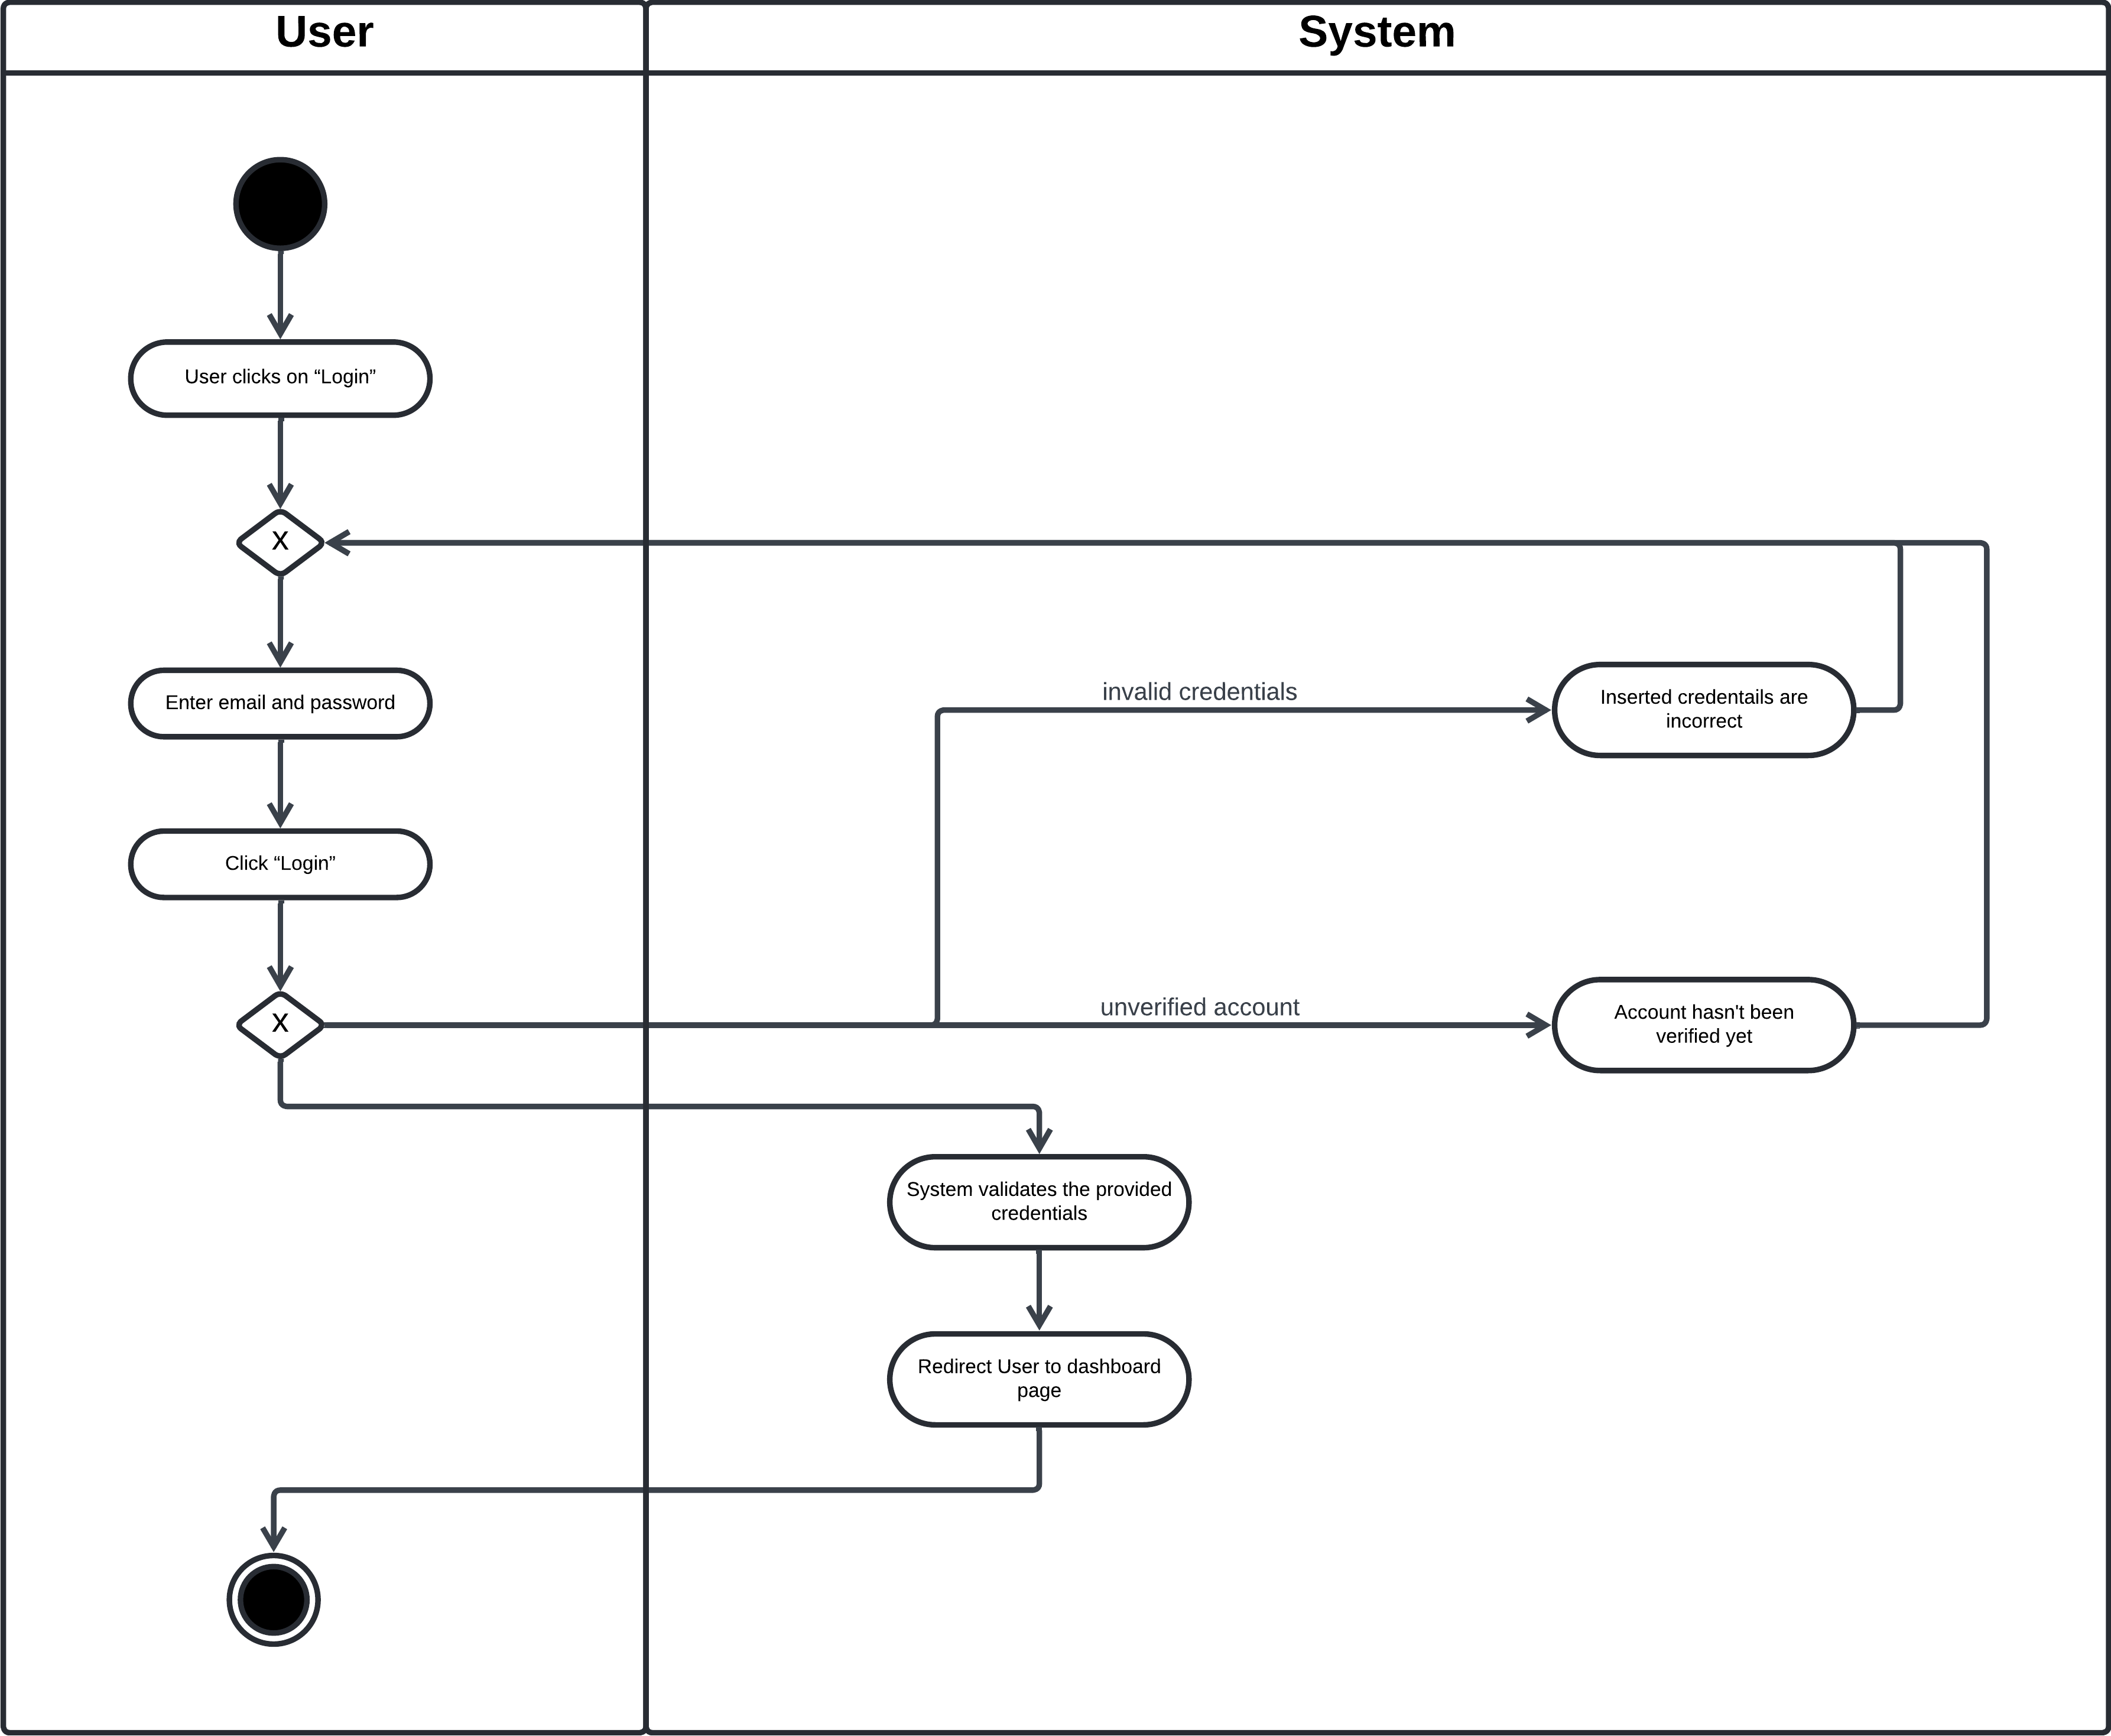
\includegraphics[width=1\linewidth]{LaTeXCode/images/activity diagram/UC4.png}
         \caption{Login by a User}
         \label{fig:login_user_ad}
     \end{center}
\end{figure}

\newpage

\subsubsection*{UC\cuc . Update User Profile}
\begin{center}
    \begin{longtable}{|l|p{0.75\linewidth}|}
        \hline
        \textbf{Actor}            & User\\
        \hline
        \textbf{Entry Conditions} & The User is logged into the S\&C platform.\\
        \hline
        \textbf{Flow of Events}   
        & \cucsteps. In their "Profile" section, the User clicks the "Edit" button. \\ 
        & \cucsteps. The User updates the desired details of its profile. \\
        & \cucsteps. The User confirms the applied changes by clicking the \newline "Apply Changes" button. \\
        & \cucsteps. If the User is a Student and the updated details are relevant, the system starts an instance of the process for identifying new recommendations via the \hyperref[subsec: generate_recommendations_uc]{\uline{UC. Generate Recommendations}} functionality. \\
        \hline
        \textbf{Exit Conditions}   & The User's profile is updated and its changes are recorded in the system. \\    
        \hline
        \textbf{Exceptions}       & \begin{itemize}
            \item Some mandatory fields are left empty: the system doesn't allow the User to complete the procedure until all the mandatory fields are filled out.
        \end{itemize}\\
        \hline
    \end{longtable}
\end{center}
\label{subsec: update_profile_uc}

\begin{figure}[H]
    \begin{center}
         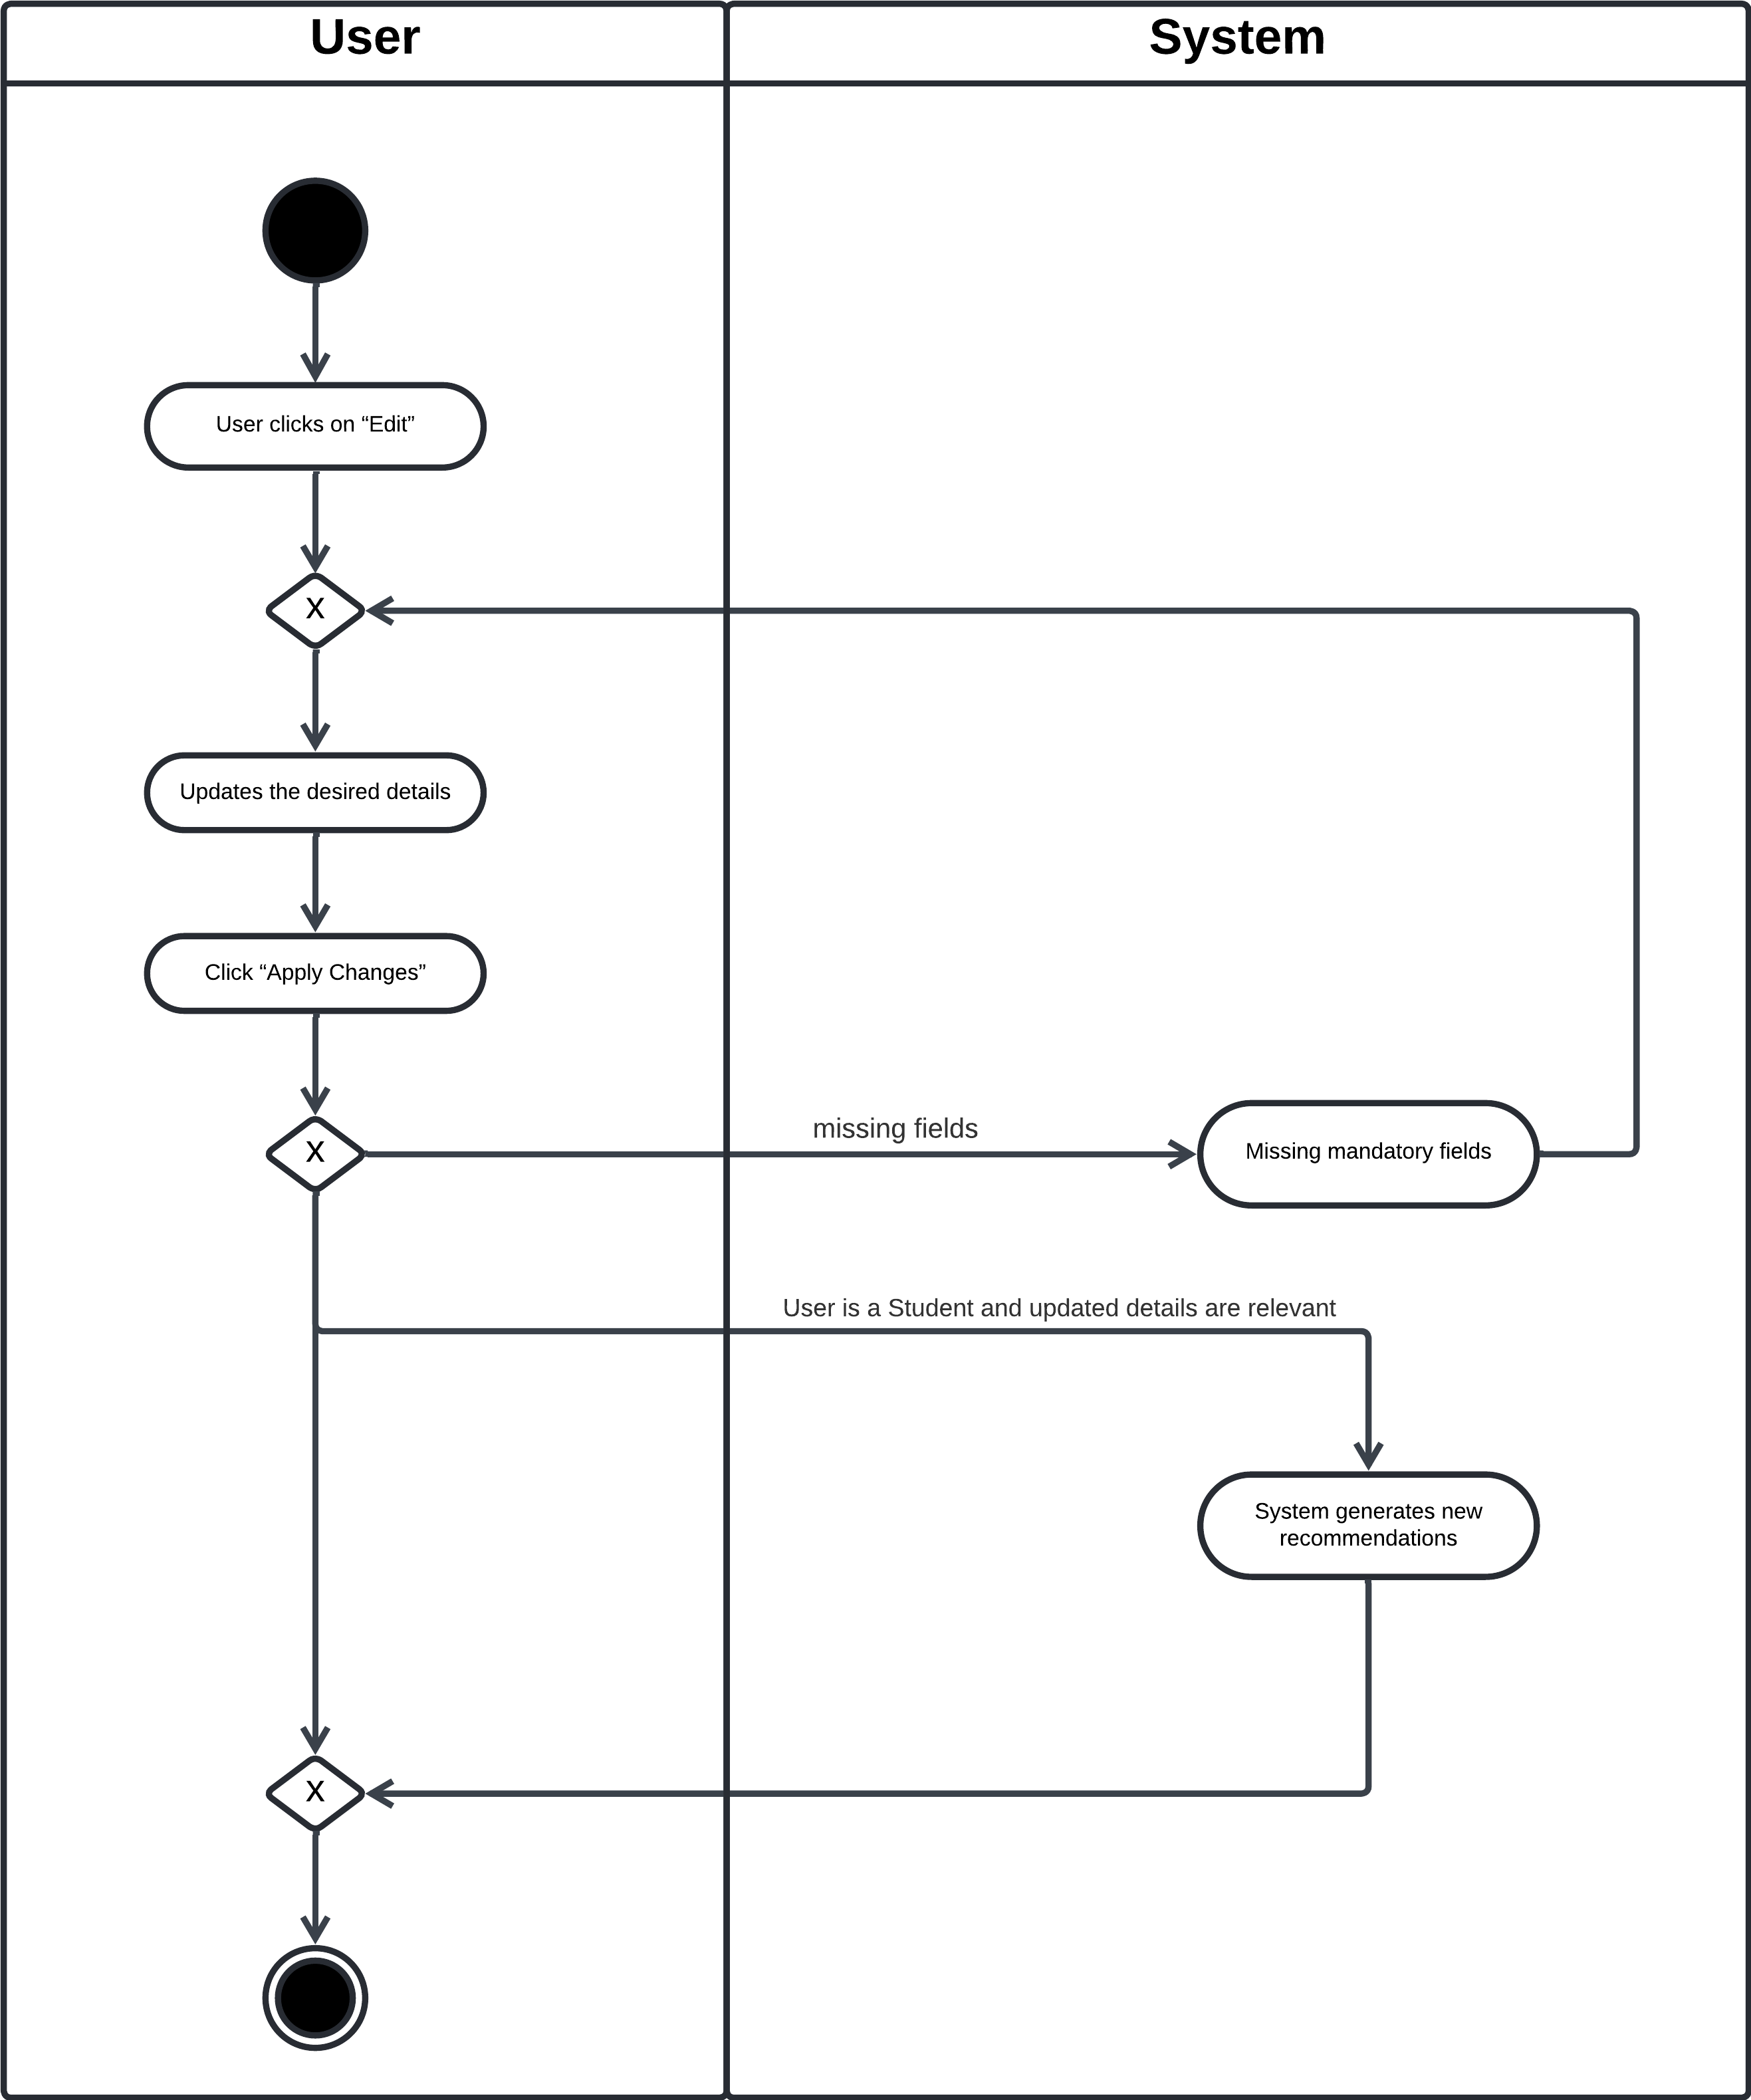
\includegraphics[width=1\linewidth]{LaTeXCode/images/activity diagram/UC5.png}
         \caption{Update User profile}
         \label{fig:update_profile_ad}
     \end{center}
\end{figure}

\newpage

\subsubsection*{UC\cuc . Publish an Internship Offer}
\begin{center}
    \begin{longtable}{|l|p{0.75\linewidth}|}
        \hline
        \textbf{Actor}            & Company \\
        \hline
        \textbf{Entry Conditions} & The Company is logged into the S\&C platform. \\
        \hline
        \textbf{Flow of Events}       
        & \cucsteps. In the dashboard, the Company clicks the "Create New Offer" button, entering the internship creation page. \\
        & \cucsteps. The Company fills out the internship creation form, inserting:
        \begin{itemize}
            \item Position
            \item Tasks to be performed
            \item Required skills
            \item Internship duration
            \item Compensation terms 
            \item Location (on-site, hybrid, or remote)
            \item Application deadline
        \end{itemize}\\
        & \cucsteps. The Company clicks the "Submit" button, waiting for the automatic data verification. \\
        & \cucsteps. The system verifies the provided data to ensure the provided information is compliant with platform guidelines, and the data is consistent and accurate. \\
        & \cucsteps. The system publishes the internship offer on the platform, making it visible to all students. \\
        & \cucsteps. The system confirms to the Company that its offer has been published. \\
        & \cucsteps. If the updated details are relevant, the system starts an instance of the process for identifying new recommendations via the \hyperref[subsec: generate_recommendations_uc]{\uline{UC. Generate Recommendations}} functionality. \\
        \hline
        \textbf{Exit Conditions}   & The internship offer is published on the platform and accessible to students. \\       
        \hline
        \textbf{Exceptions}       & \begin{itemize}
            \item Some mandatory fields are missing: the system doesn’t allow the Company to complete the procedure until all the mandatory fields are filled out.
            \item Some information is not compliant with platform guidelines: the system alerts the Company about the issue and requires revisions.
        \end{itemize} \\
        \hline
    \end{longtable}
\end{center}

\begin{figure}[H]
    \begin{center}
         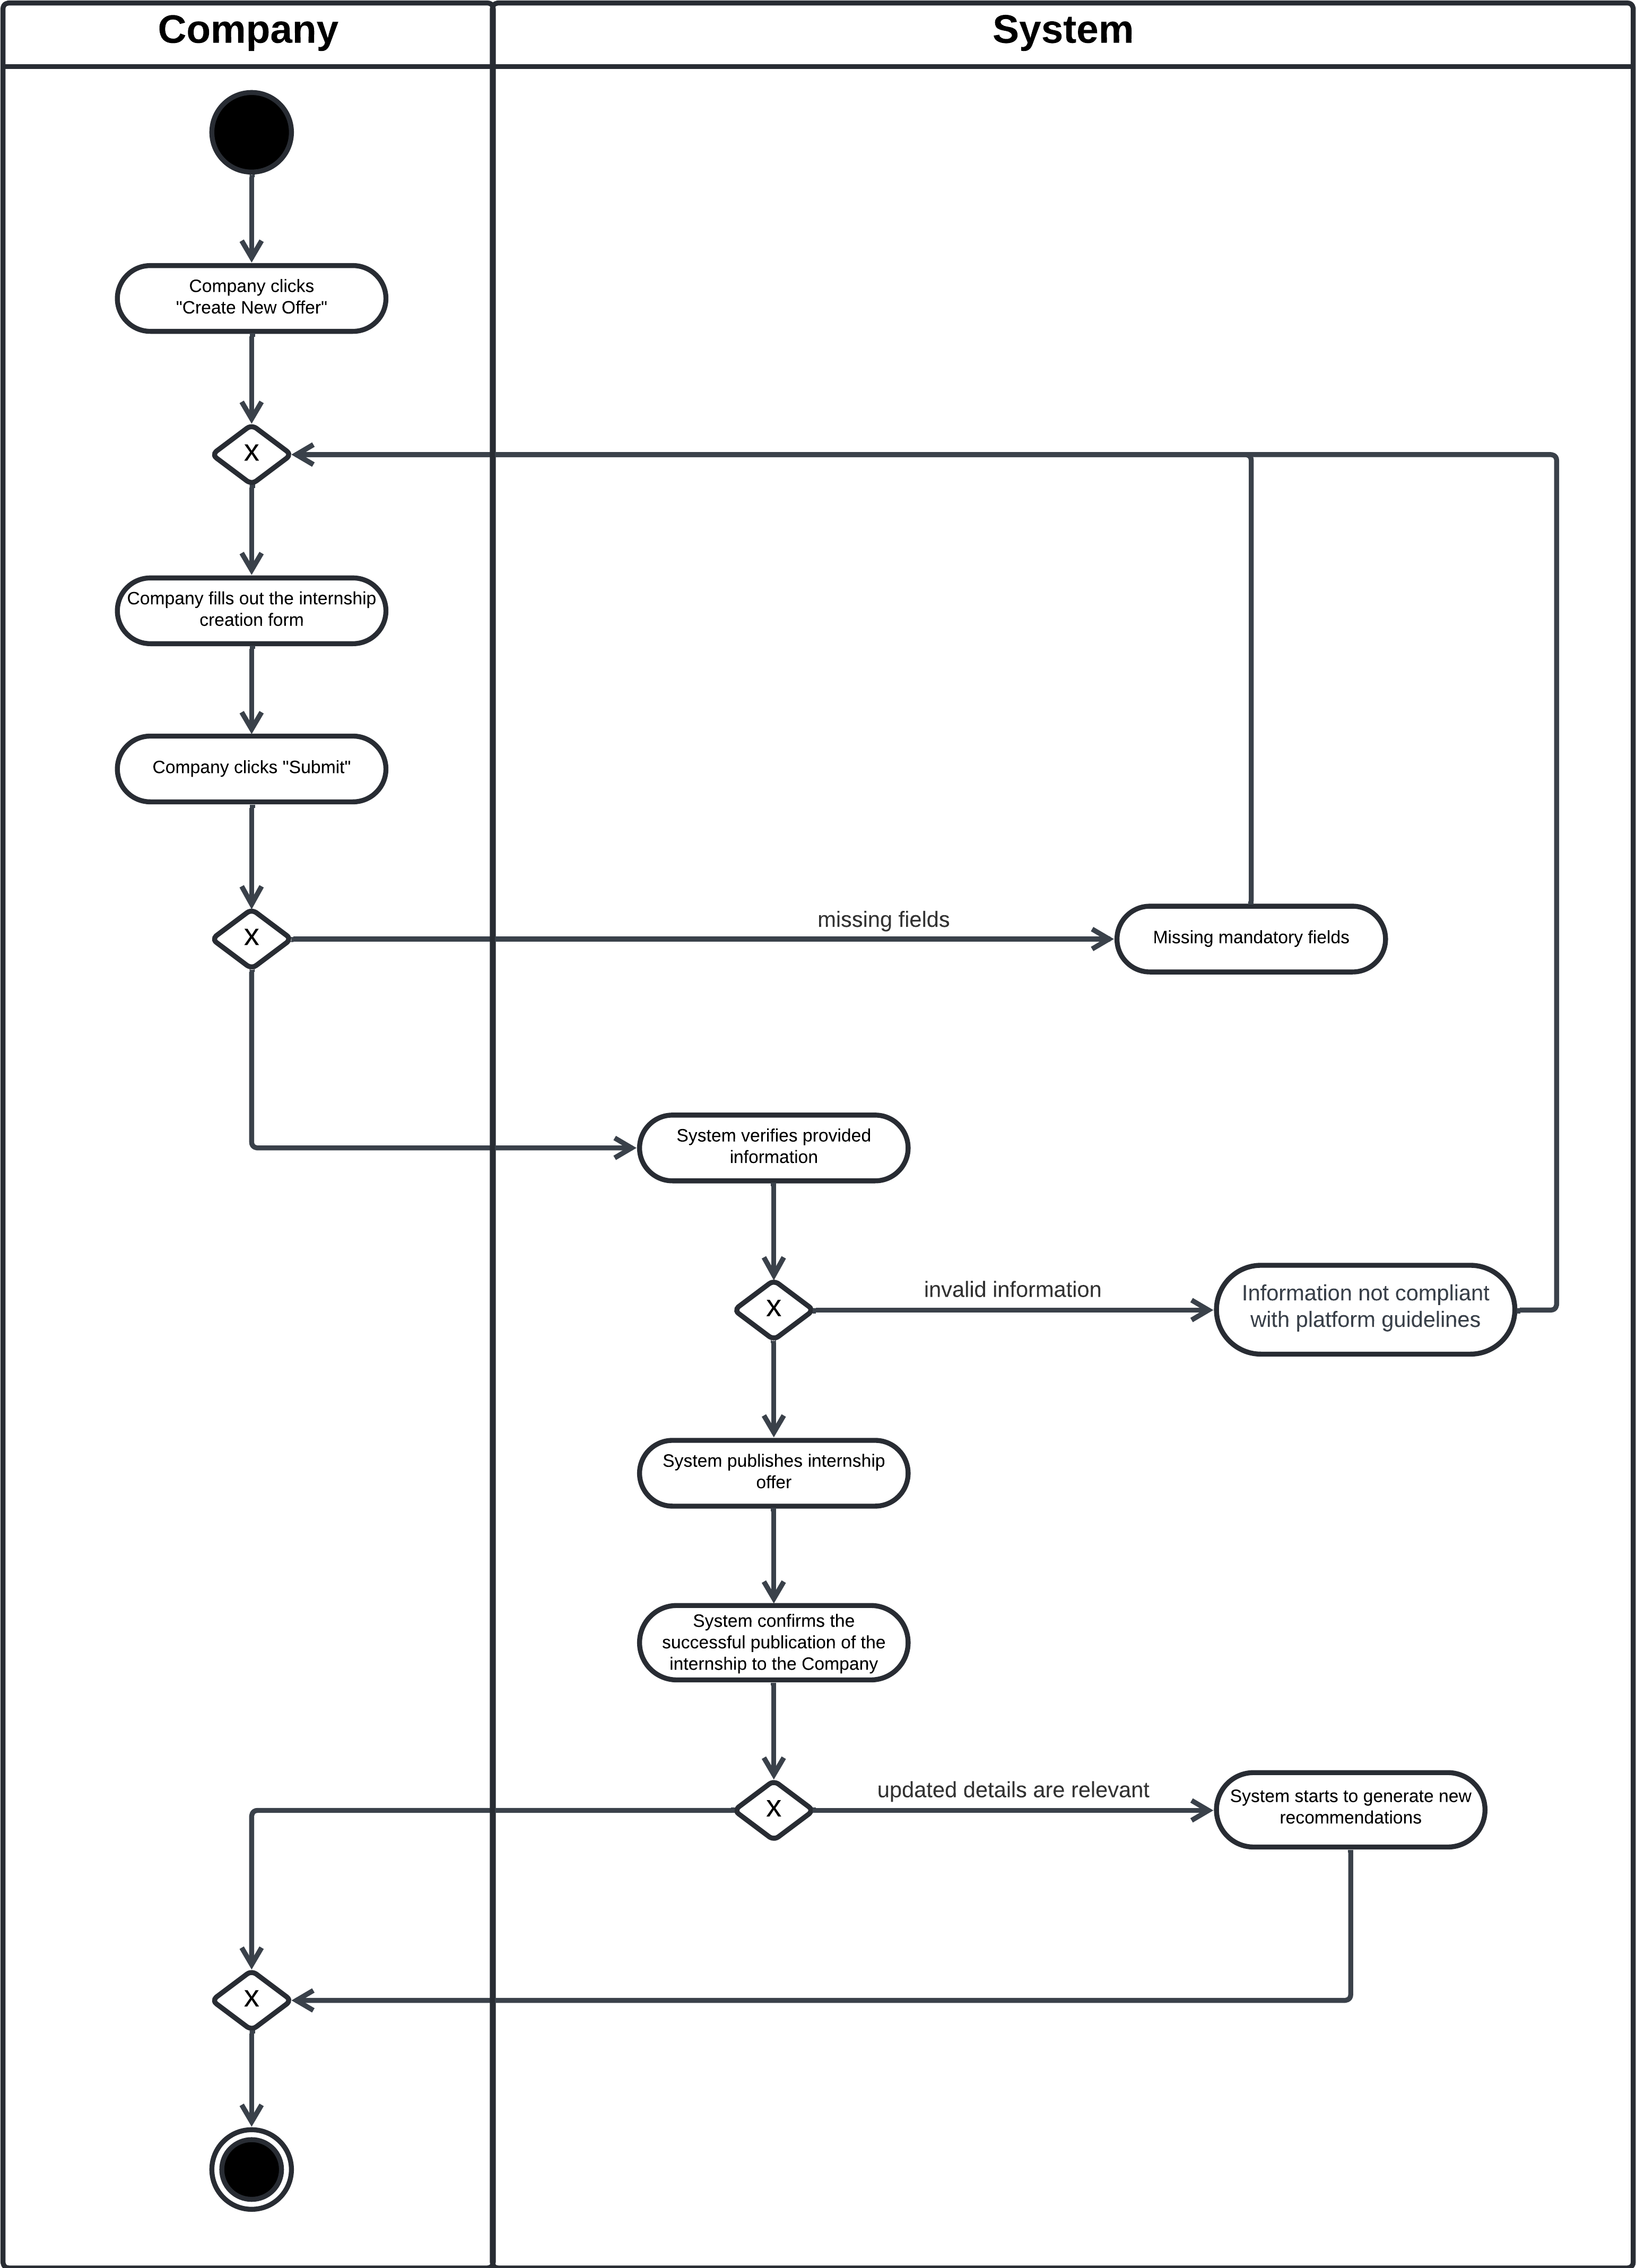
\includegraphics[width=1\linewidth]{LaTeXCode/images/activity diagram/UC6.png}
         \caption{Publish an Internship Offer}
         \label{fig:publish_offer_ad}
     \end{center}
\end{figure}

\newpage

\subsubsection*{UC\cuc . Update Internship Offer}
\begin{center}
    \begin{longtable}{|l|p{0.75\linewidth}|}
        \hline
        \textbf{Actor}            & Company\\
        \hline
        \textbf{Entry Conditions} & The Company is logged into the S\&C platform and the selected internship offer’s application deadline has not expired yet.\\
        \hline
        \textbf{Flow of Events}   
        & \cucsteps. On the selected internship offer's page, the Company clicks the "Edit" button. \\ 
        & \cucsteps. The Company updates the desired details of the internship offer or chooses to withdraw it entirely by clicking the "Withdraw Offer" button. \\
        & \theucsteps. The Company acts accordingly based on their decision: \\
        & \theucsteps.1. If the Company updates the details, it confirms the applied changes by clicking the "Apply Changes" button. \\
        & \cucsteps.2. If the Company chooses to withdraw the offer, a confirmation prompt appears, asking to finalize the withdrawal. Upon confirmation, the internship offer is marked as "Closed" and becomes inaccessible to students. \\
        & \theucsteps.1. If updates are confirmed, the system records the changes. \\
        & \cucsteps.2. If the offer is withdrawn, the system cancels all pending processes related to the offer, such as identifying new recommendations or managing applications. \\
        & \cucsteps. For an updated offer, the system starts an instance of the process for identifying new recommendations via the \hyperref[subsec: generate_recommendations_uc]{\uline{UC. Generate Recommendations}} functionality. \\
        \hline
        \textbf{Exit Conditions}   & The selected internship offer is updated and its changes are recorded in the system. \\    
        \hline
        \textbf{Exceptions}       & \begin{itemize}
            \item Some mandatory fields are missing: the system doesn't allow the Company to complete the procedure until all the mandatory fields are filled out.
            \item Some information is not compliant with platform guidelines: the system alerts the Company about the issue and requires revisions.
        \end{itemize}\\
        \hline
    \end{longtable}
\end{center}
\label{subsec: update_internship_offer_uc}

\begin{figure}[H]
    \begin{center}
         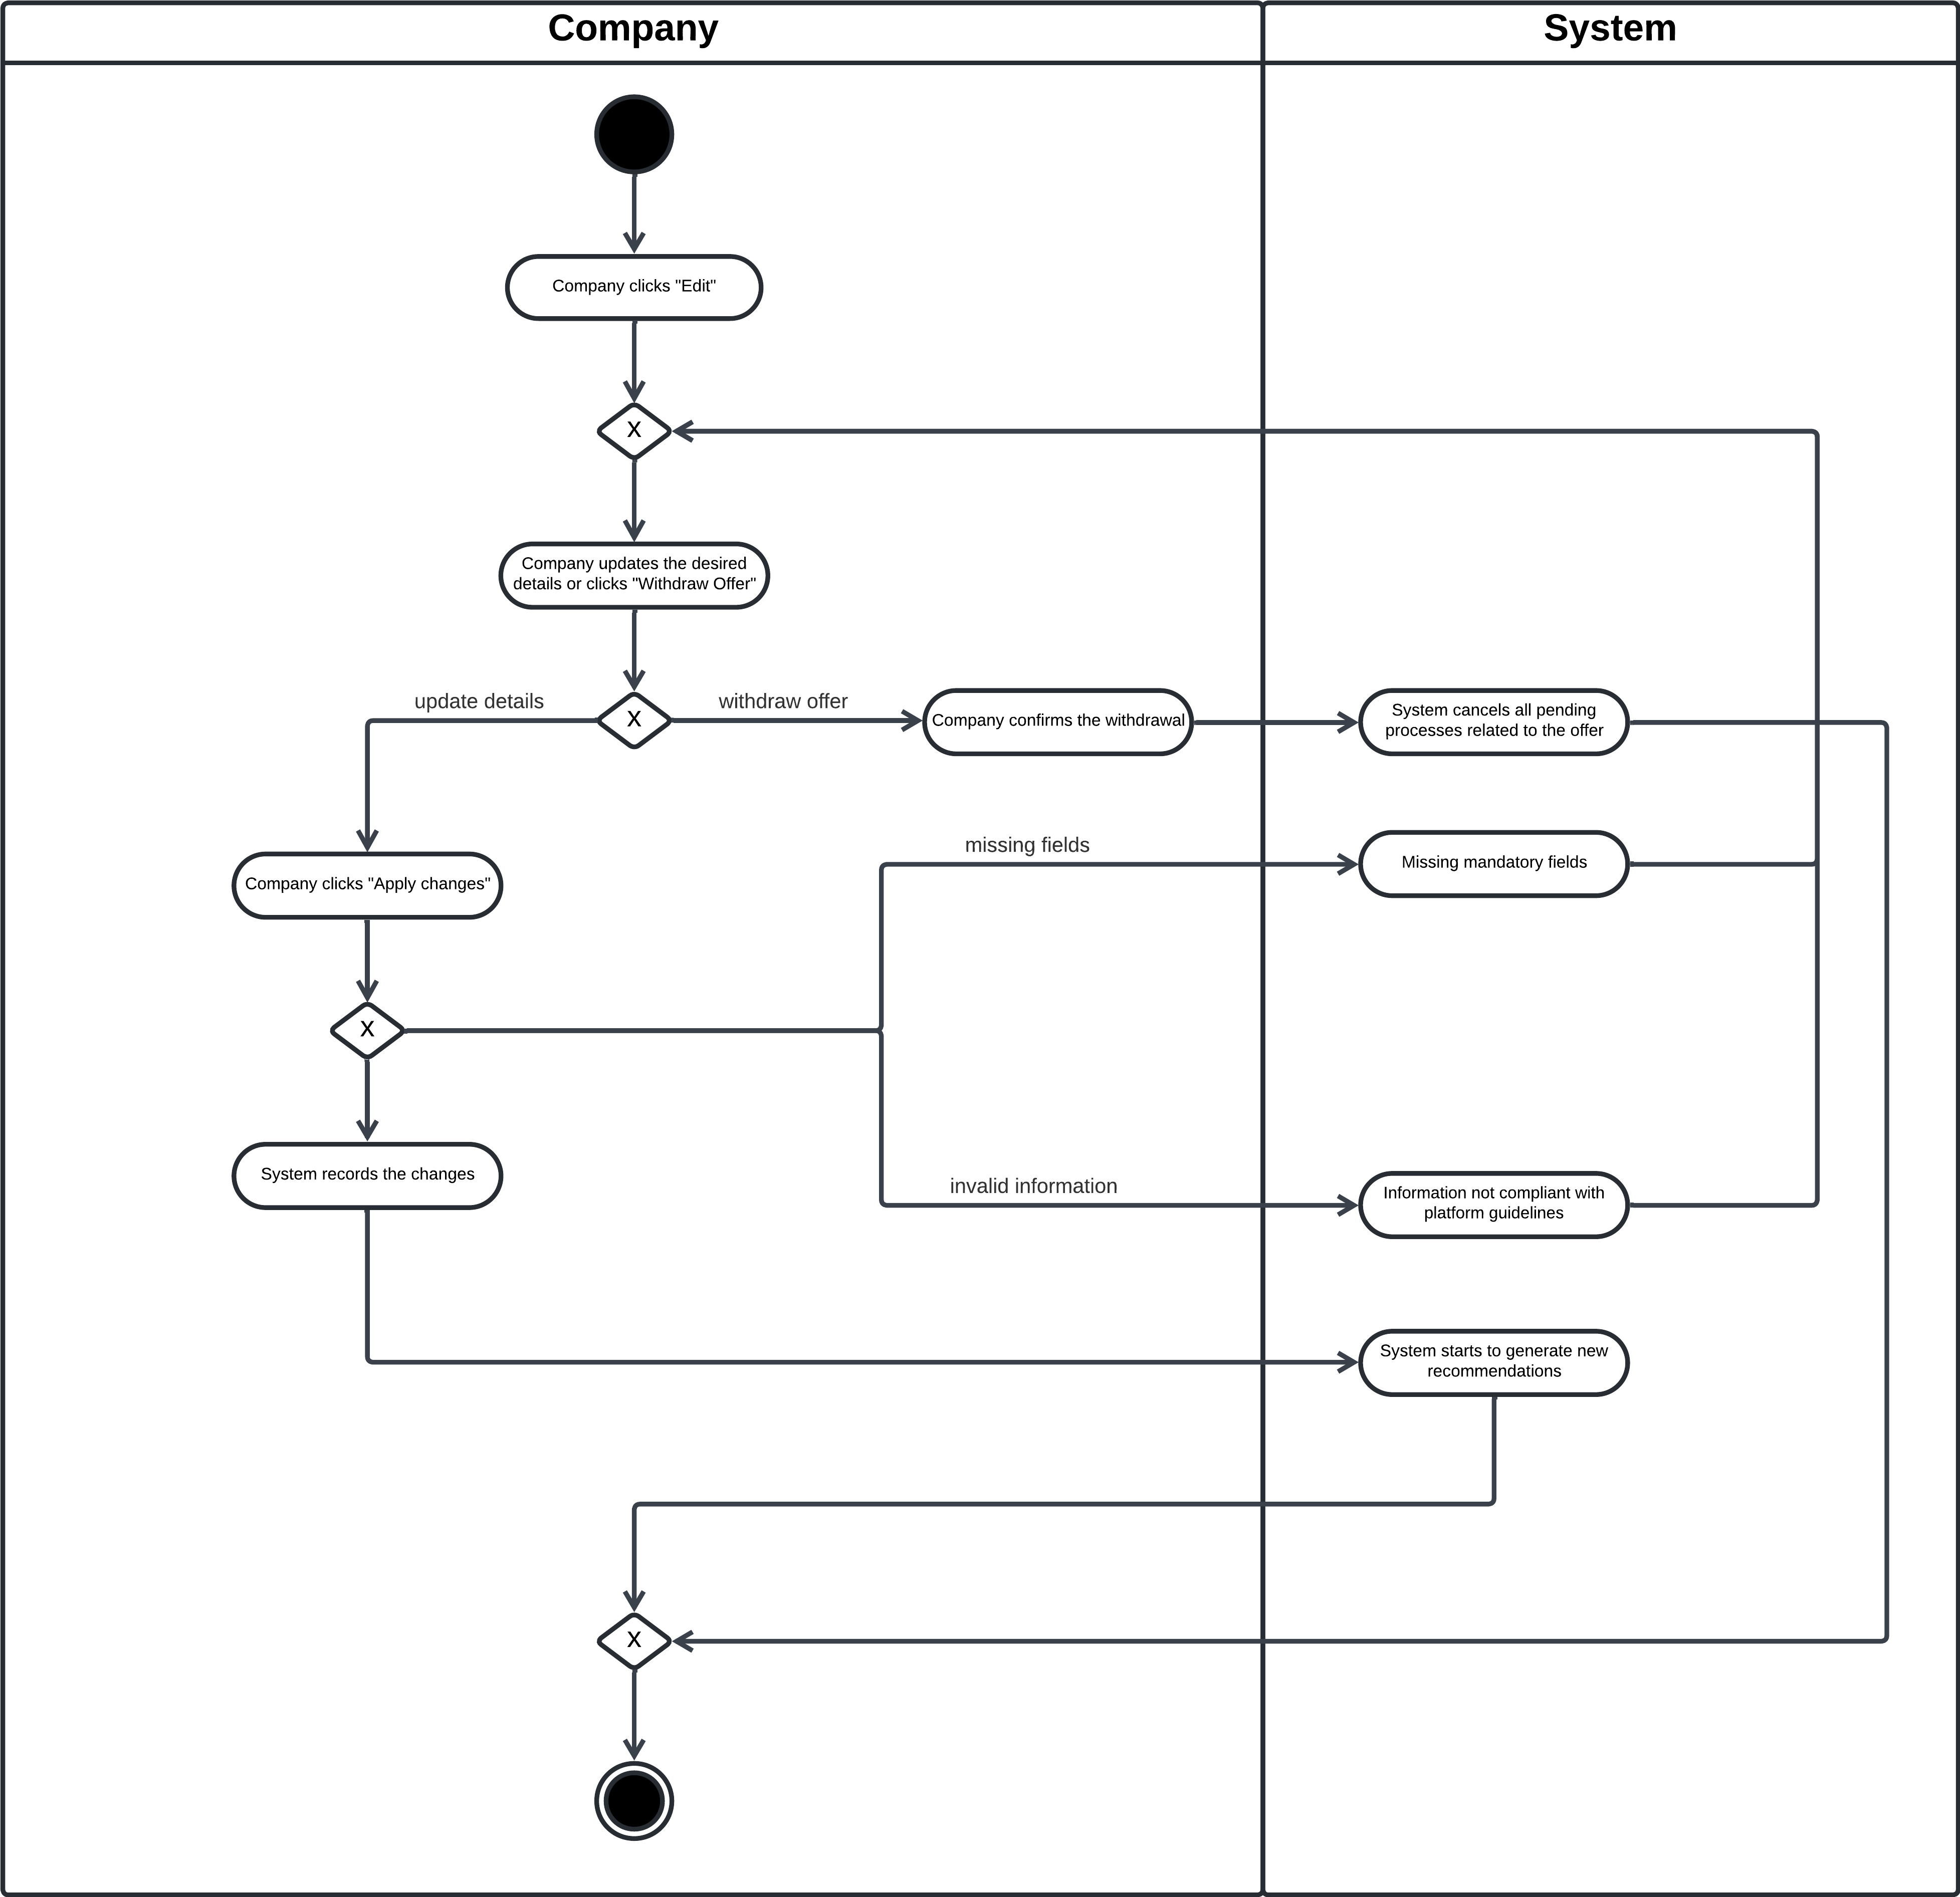
\includegraphics[width=1\linewidth]{LaTeXCode/images/activity diagram/UC7.png}
         \caption{Update Internship Offer}
         \label{fig:update_internship_offer_ad}
     \end{center}
\end{figure}

\newpage

\subsubsection*{UC\cuc . Search Internship Offers}
\begin{center}
    \begin{longtable}{|l|p{0.75\linewidth}|}
        \hline
        \textbf{Actor}            & Student \\
        \hline
        \textbf{Entry Conditions} & The Student is logged into the S\&C platform. \\
        \hline
        \textbf{Flow of Events}       
        & \cucsteps. In the dashboard, the Student navigates to the "Search Offers" section. \\
        & \cucsteps. The system displays a search interface which has the following optional filters:
        \begin{itemize}
            \item Domain of interest
            \item Location (on-site, hybrid, or remote)
            \item Internship duration
            \item Compensation terms
            \item Keywords (an offer matches a keyword if it contains that keyword or a semantically similar one in any of its fields).
        \end{itemize}\\
        & \cucsteps. The Student selects the desired filters and submits the query to the system. \\
        & \cucsteps. The system retrieves and displays a list of internship offers that match the selected criteria. \\
        & \cucsteps. Optionally, the Student applies one or more ordering criteria: newest, oldest, most relevant, or most number of applications, by selecting the desired ones from a drop-down list. \\
        \hline
        \textbf{Exit Conditions}   & The system displays the list of internship offers matching the given criteria. \\ 
        \hline
        \textbf{Exceptions}       & \begin{itemize}
            \item The system doesn't find any matching result: if none of the active internship offers matches the selected criteria, the system displays a message indicating it.
        \end{itemize}\\
        \hline
    \end{longtable}
\end{center}

\begin{figure}[H]
    \begin{center}
         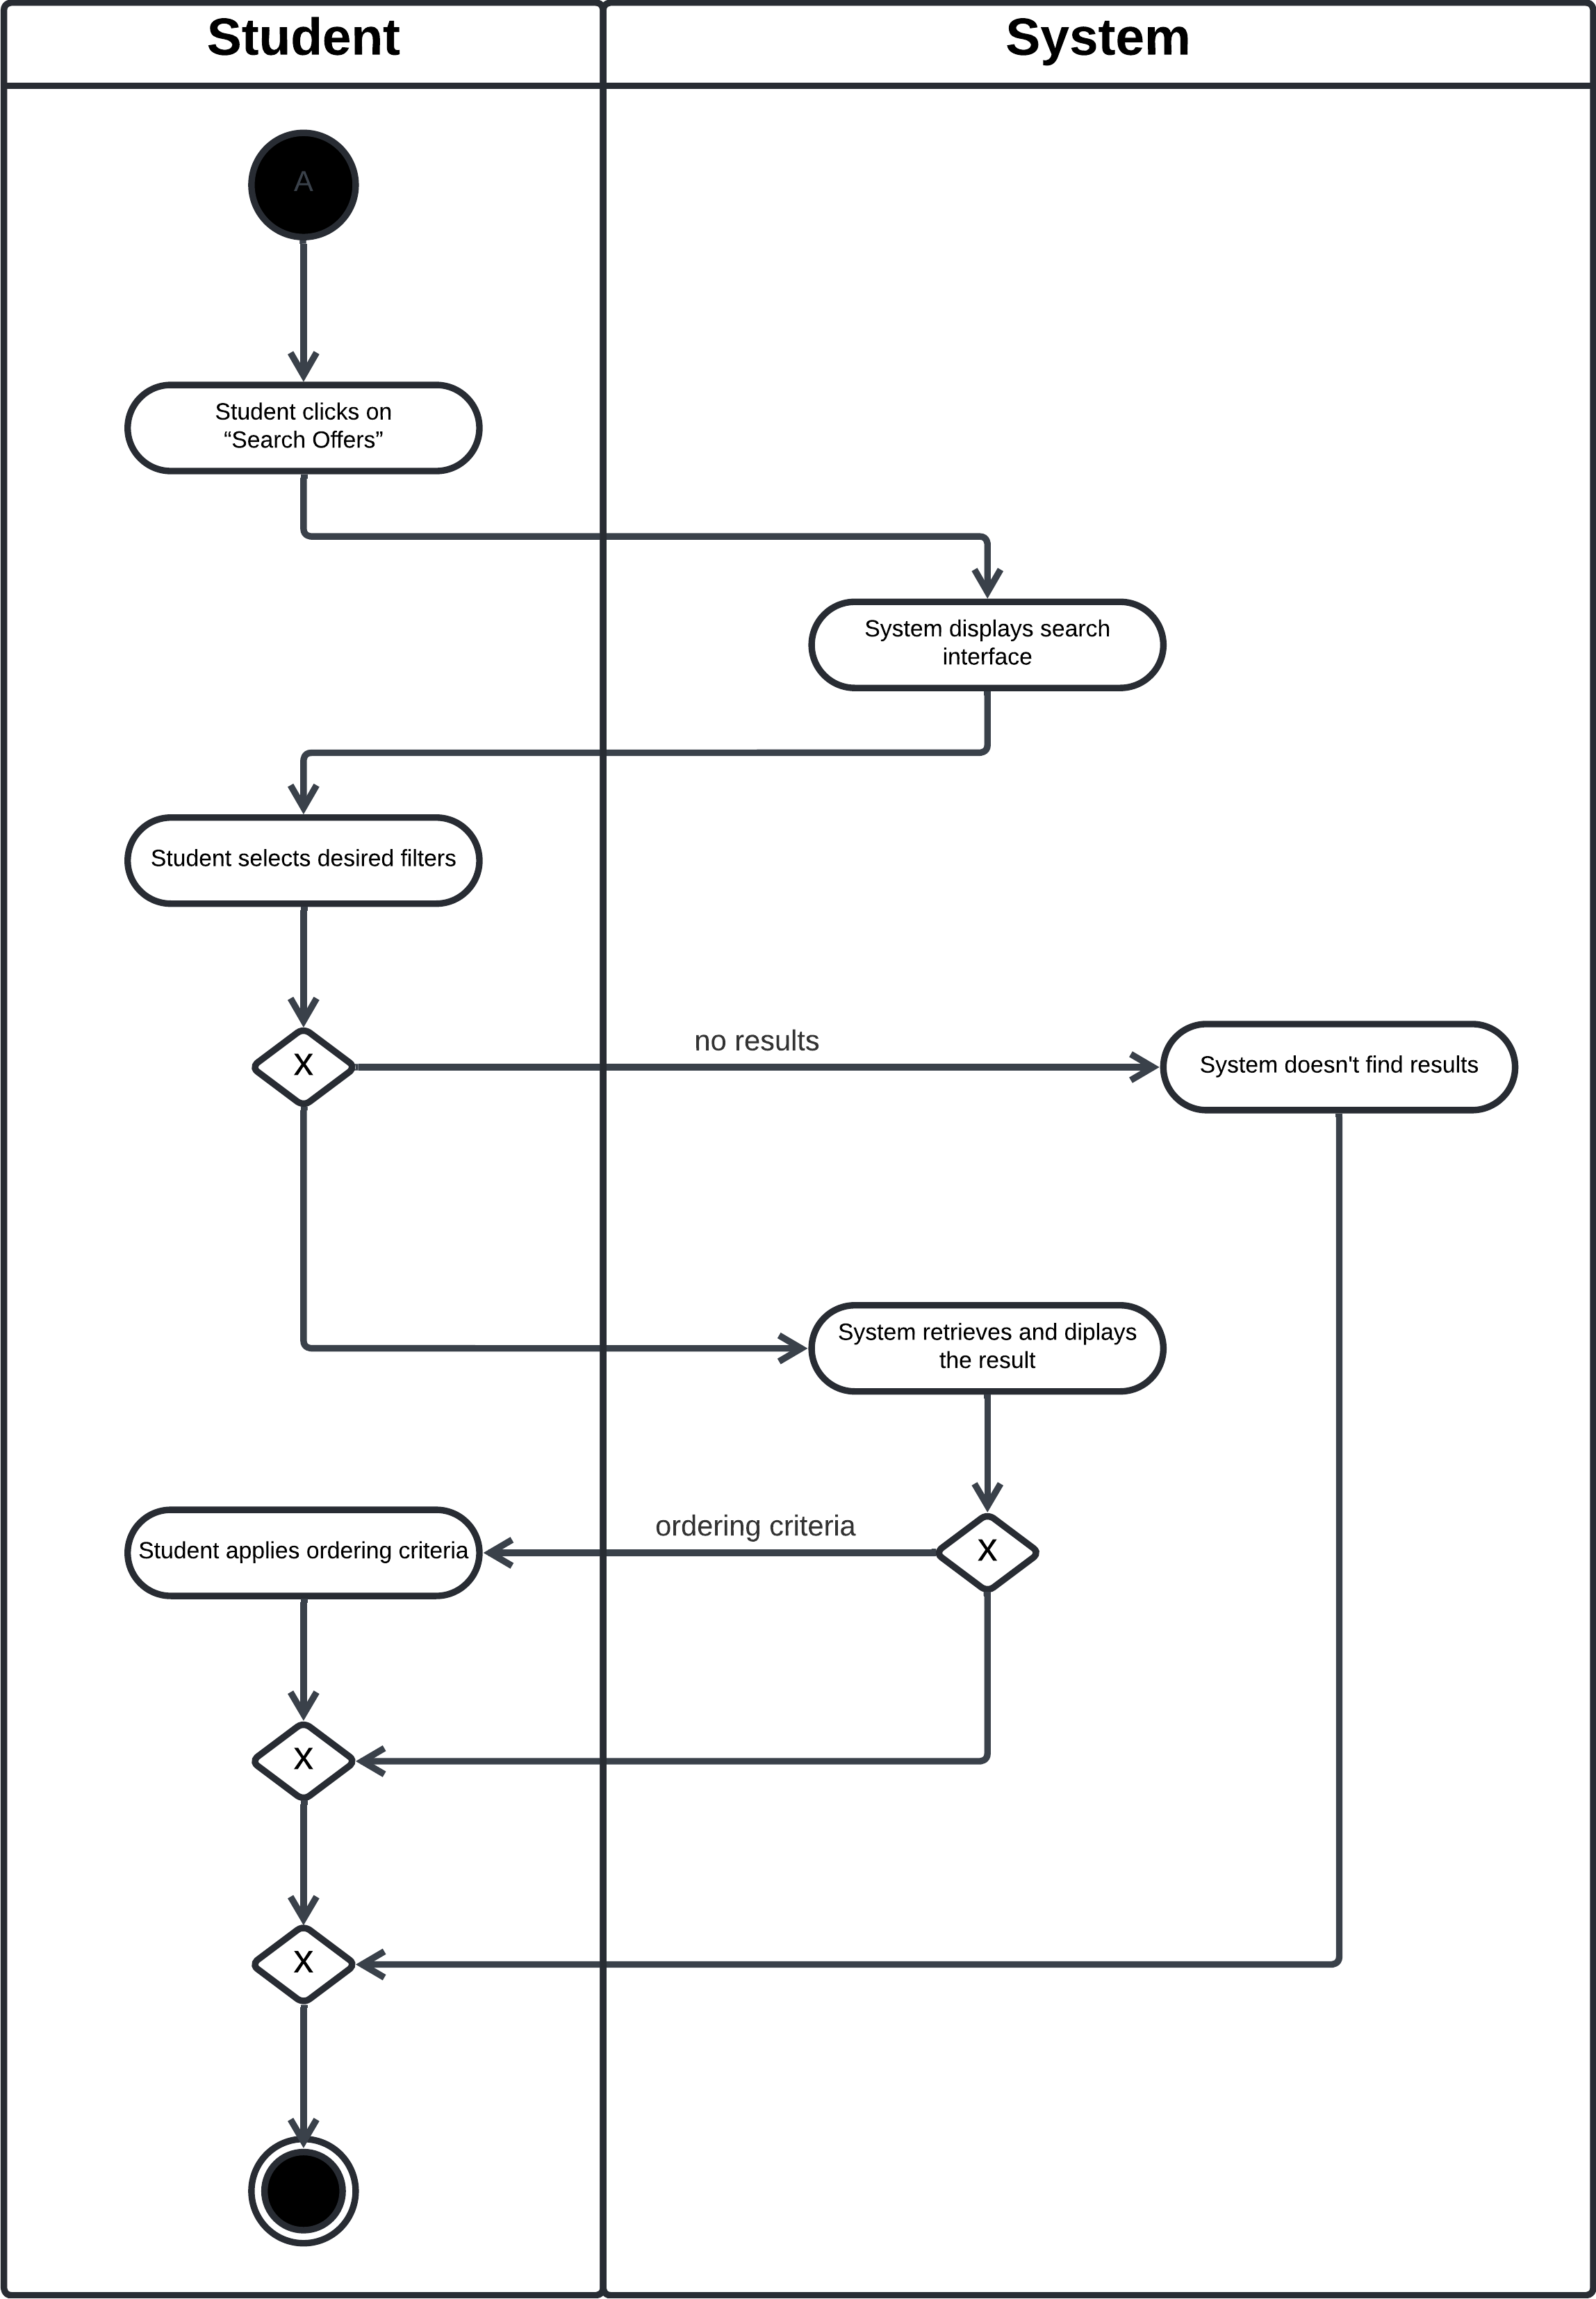
\includegraphics[width=1\linewidth]{LaTeXCode/images/activity diagram/UC8.png}
         \caption{Search Internship Offers}
         \label{fig:search_offer_ad}
     \end{center}
\end{figure}

\newpage

\subsubsection*{UC\cuc . Apply to an Internship Offer}
\begin{center}
    \begin{longtable}{|l|p{0.75\linewidth}|}
        \hline
        \textbf{Actor}            & Student \\
        \hline
        \textbf{Entry Conditions} & The Student is logged into the S\&C platform and is on the page of an internship offer. \\
        \hline
        \textbf{Flow of Events}       
        & \cucsteps. On the internship offer page, the Student clicks the "Apply" button. \\
        & \cucsteps. The system adds the application to the internship offer's candidates list. \\
        & \cucsteps. The system marks all the "Unhandled" recommendations of the Student about the selected internship offer as "Accepted" and discards all the "Unhandled" recommendations of the offering Company about them. \\
        & \cucsteps. The system confirms to the Student that the application has been successfully registered into the system. \\
        \hline
        \textbf{Exit Conditions}   & The Student has successfully made an application to an internship offer of his choice. \\
        \hline
        \textbf{Exceptions}       & \begin{itemize}
            \item The deadline for applying to the internship has expired: the "Apply" button cannot be clicked and the Student has to give up on applying.
        \end{itemize}\\
        \hline
    \end{longtable}
\end{center}
\label{subsec: apply_to_internships_uc}

\begin{figure}[H]
    \begin{center}
         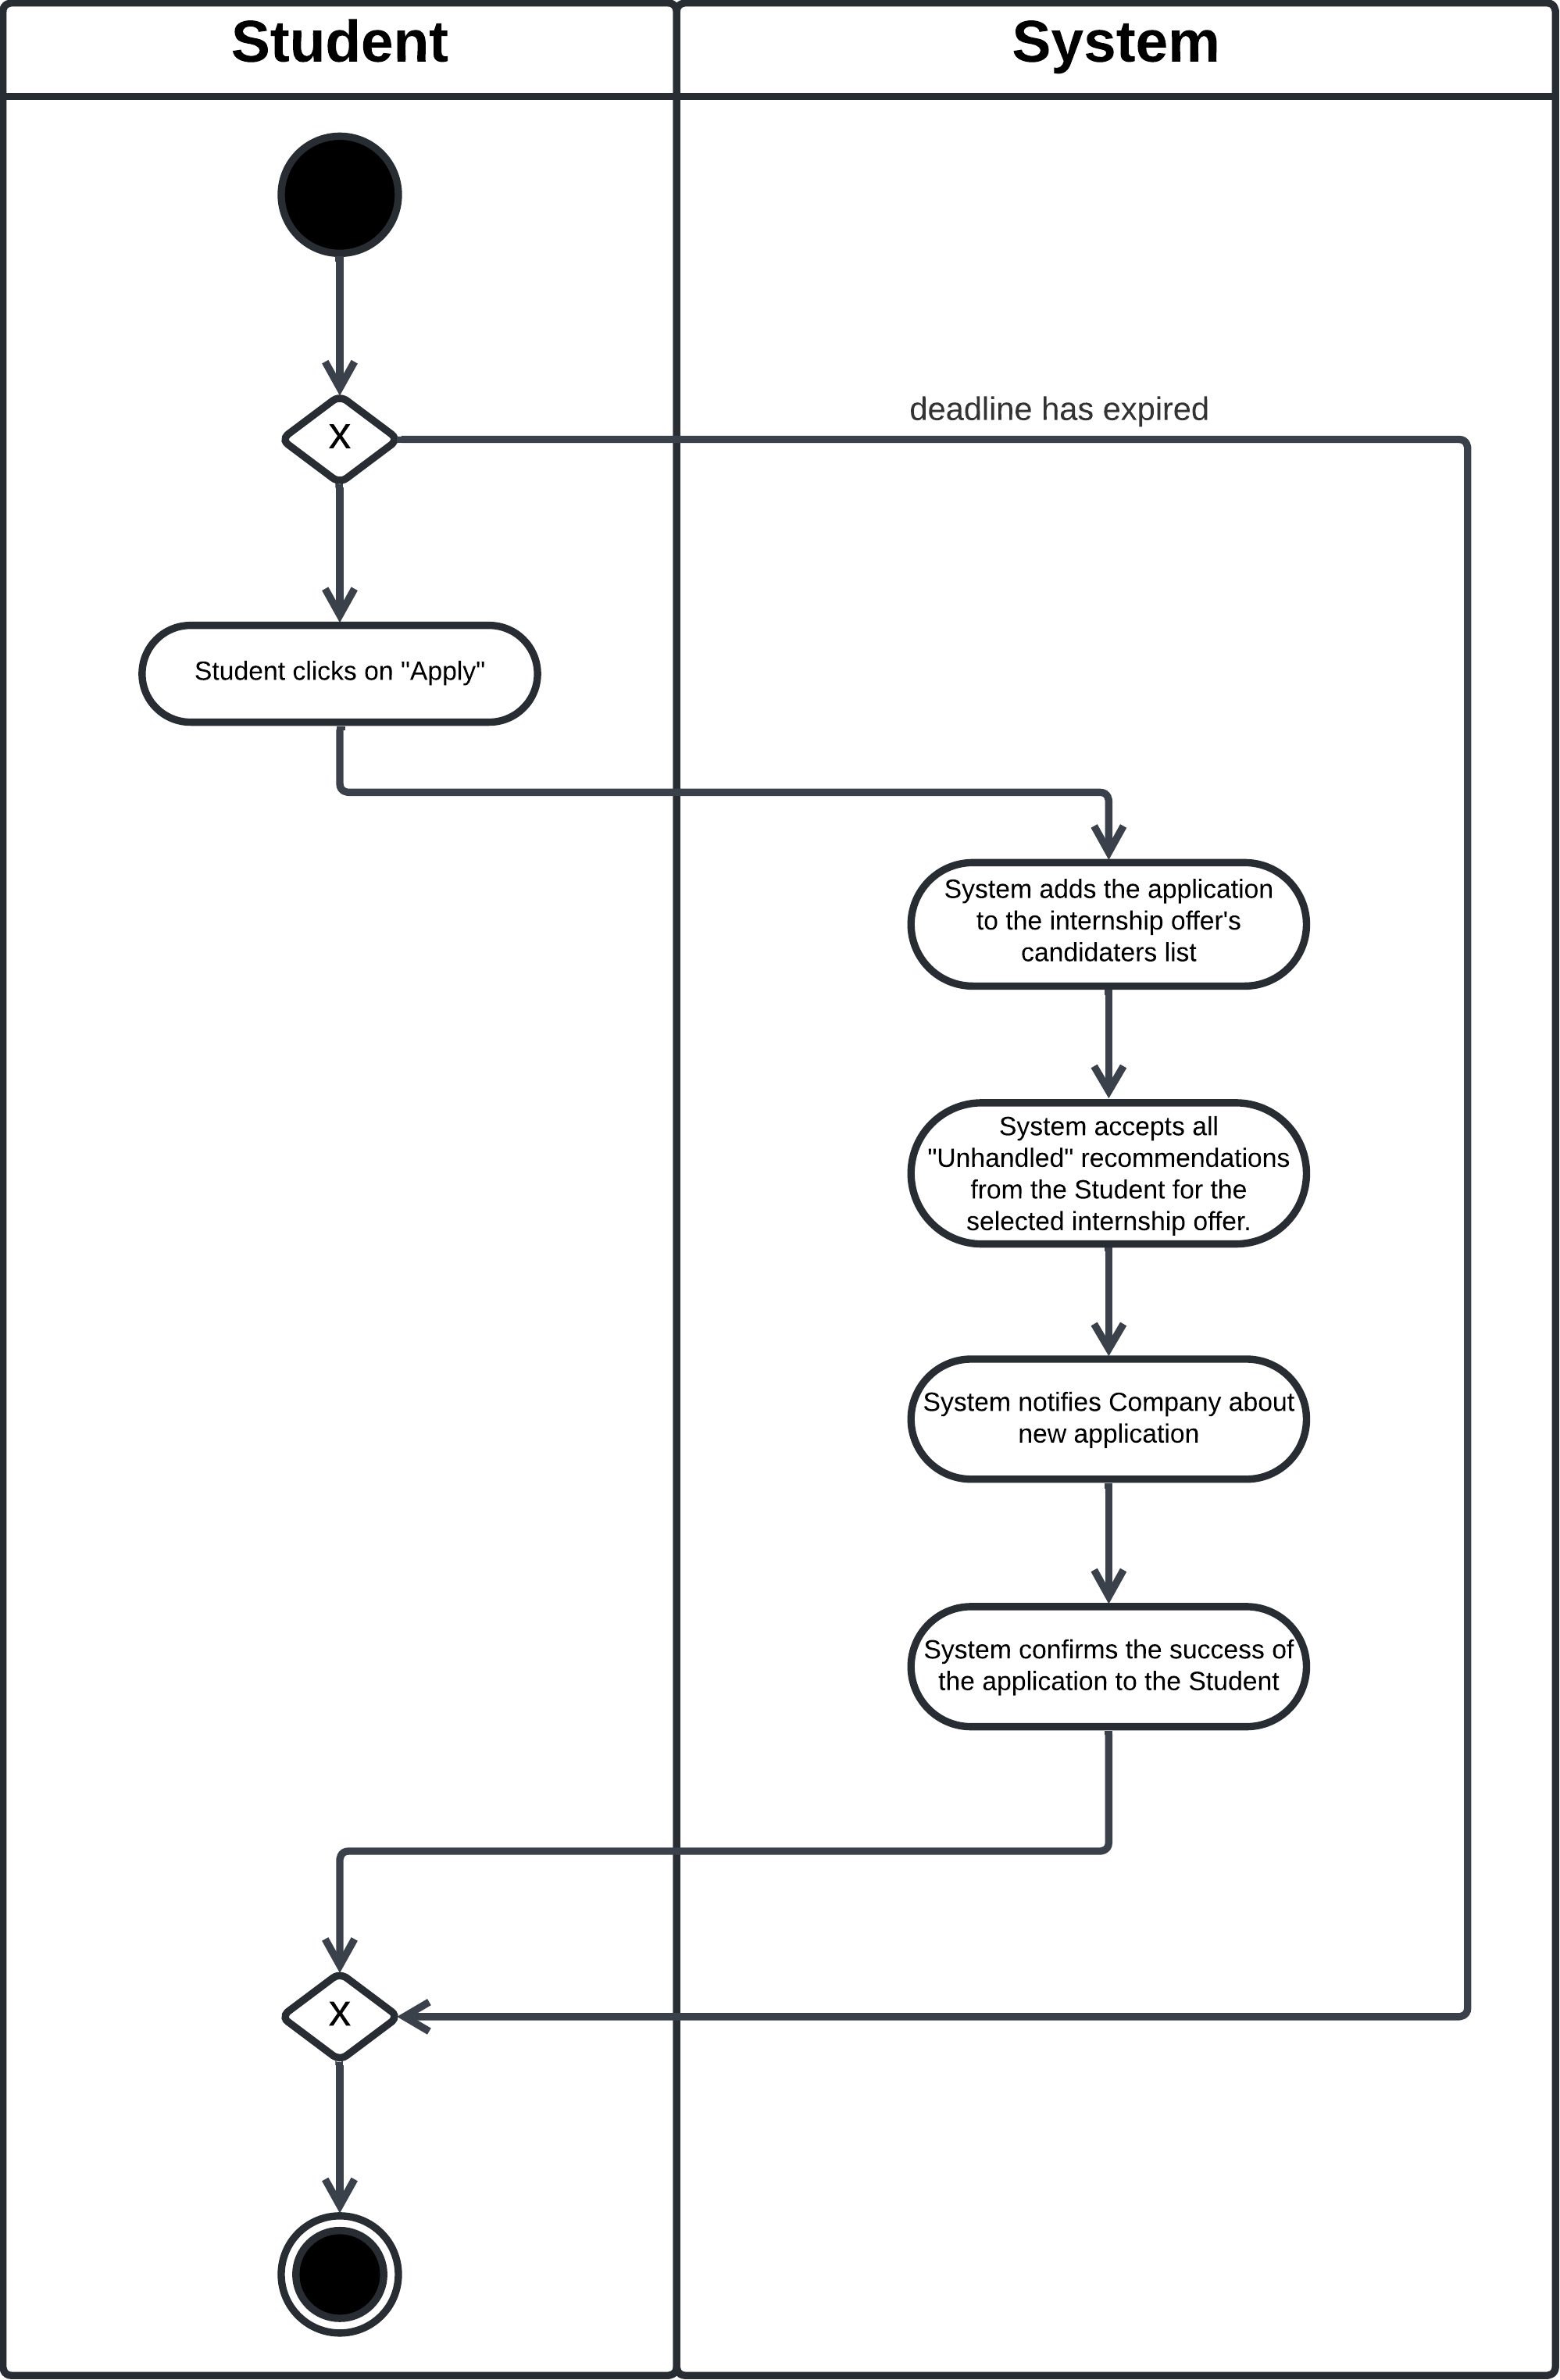
\includegraphics[width=0.9\linewidth]{LaTeXCode/images/activity diagram/UC9.png}
         \caption{Apply to an Internship Offer}
         \label{fig:apply_to_internships_ad}
     \end{center}
\end{figure}

\newpage

\subsubsection*{UC\cuc . Generate Recommendations}
\begin{center}
    \begin{longtable}{|l|p{0.75\linewidth}|}
        \hline
        \textbf{Actor}            & None\\
        \hline
        \textbf{Entry Conditions} & A relevant change in the system's information set has occurred, with the possibility of new matches between a Student and a Company emerging. \\
        \hline
        \textbf{Flow of Events}
        & \cucsteps. By taking into account the newly updated information and a subset of information from all the students, internship offers and companies, including feedback previously expressed by the parties on the platform, the system identifies every new potential match between a Student and an internship offer by a Company that has arisen as a consequence of the update of the information set and had never been identified before. In order to be considered, a match that had already been identified previously and subsequently discarded by a Party needs to have been generated by a substantial change in the information set (with the threshold possibly increasing). \\ 
        & \cucsteps. For every new match, the system generates a recommendation for the identified Parties, which could be only the Student, only the Company or both. Then, the system adds it to the list of recommendations of such Parties. \\
        \hline
        \textbf{Exit Condition}   & The generated recommendations have been posted on the respective Parties' dashboards. \\       
        \hline
        \textbf{Exceptions}       & \begin{itemize}
            \item The system doesn't find any match: it terminates the process silently. 
        \end{itemize}\\
        \hline
    \end{longtable}
\end{center}
\label{subsec: generate_recommendations_uc}

\begin{figure}[H]
    \begin{center}
         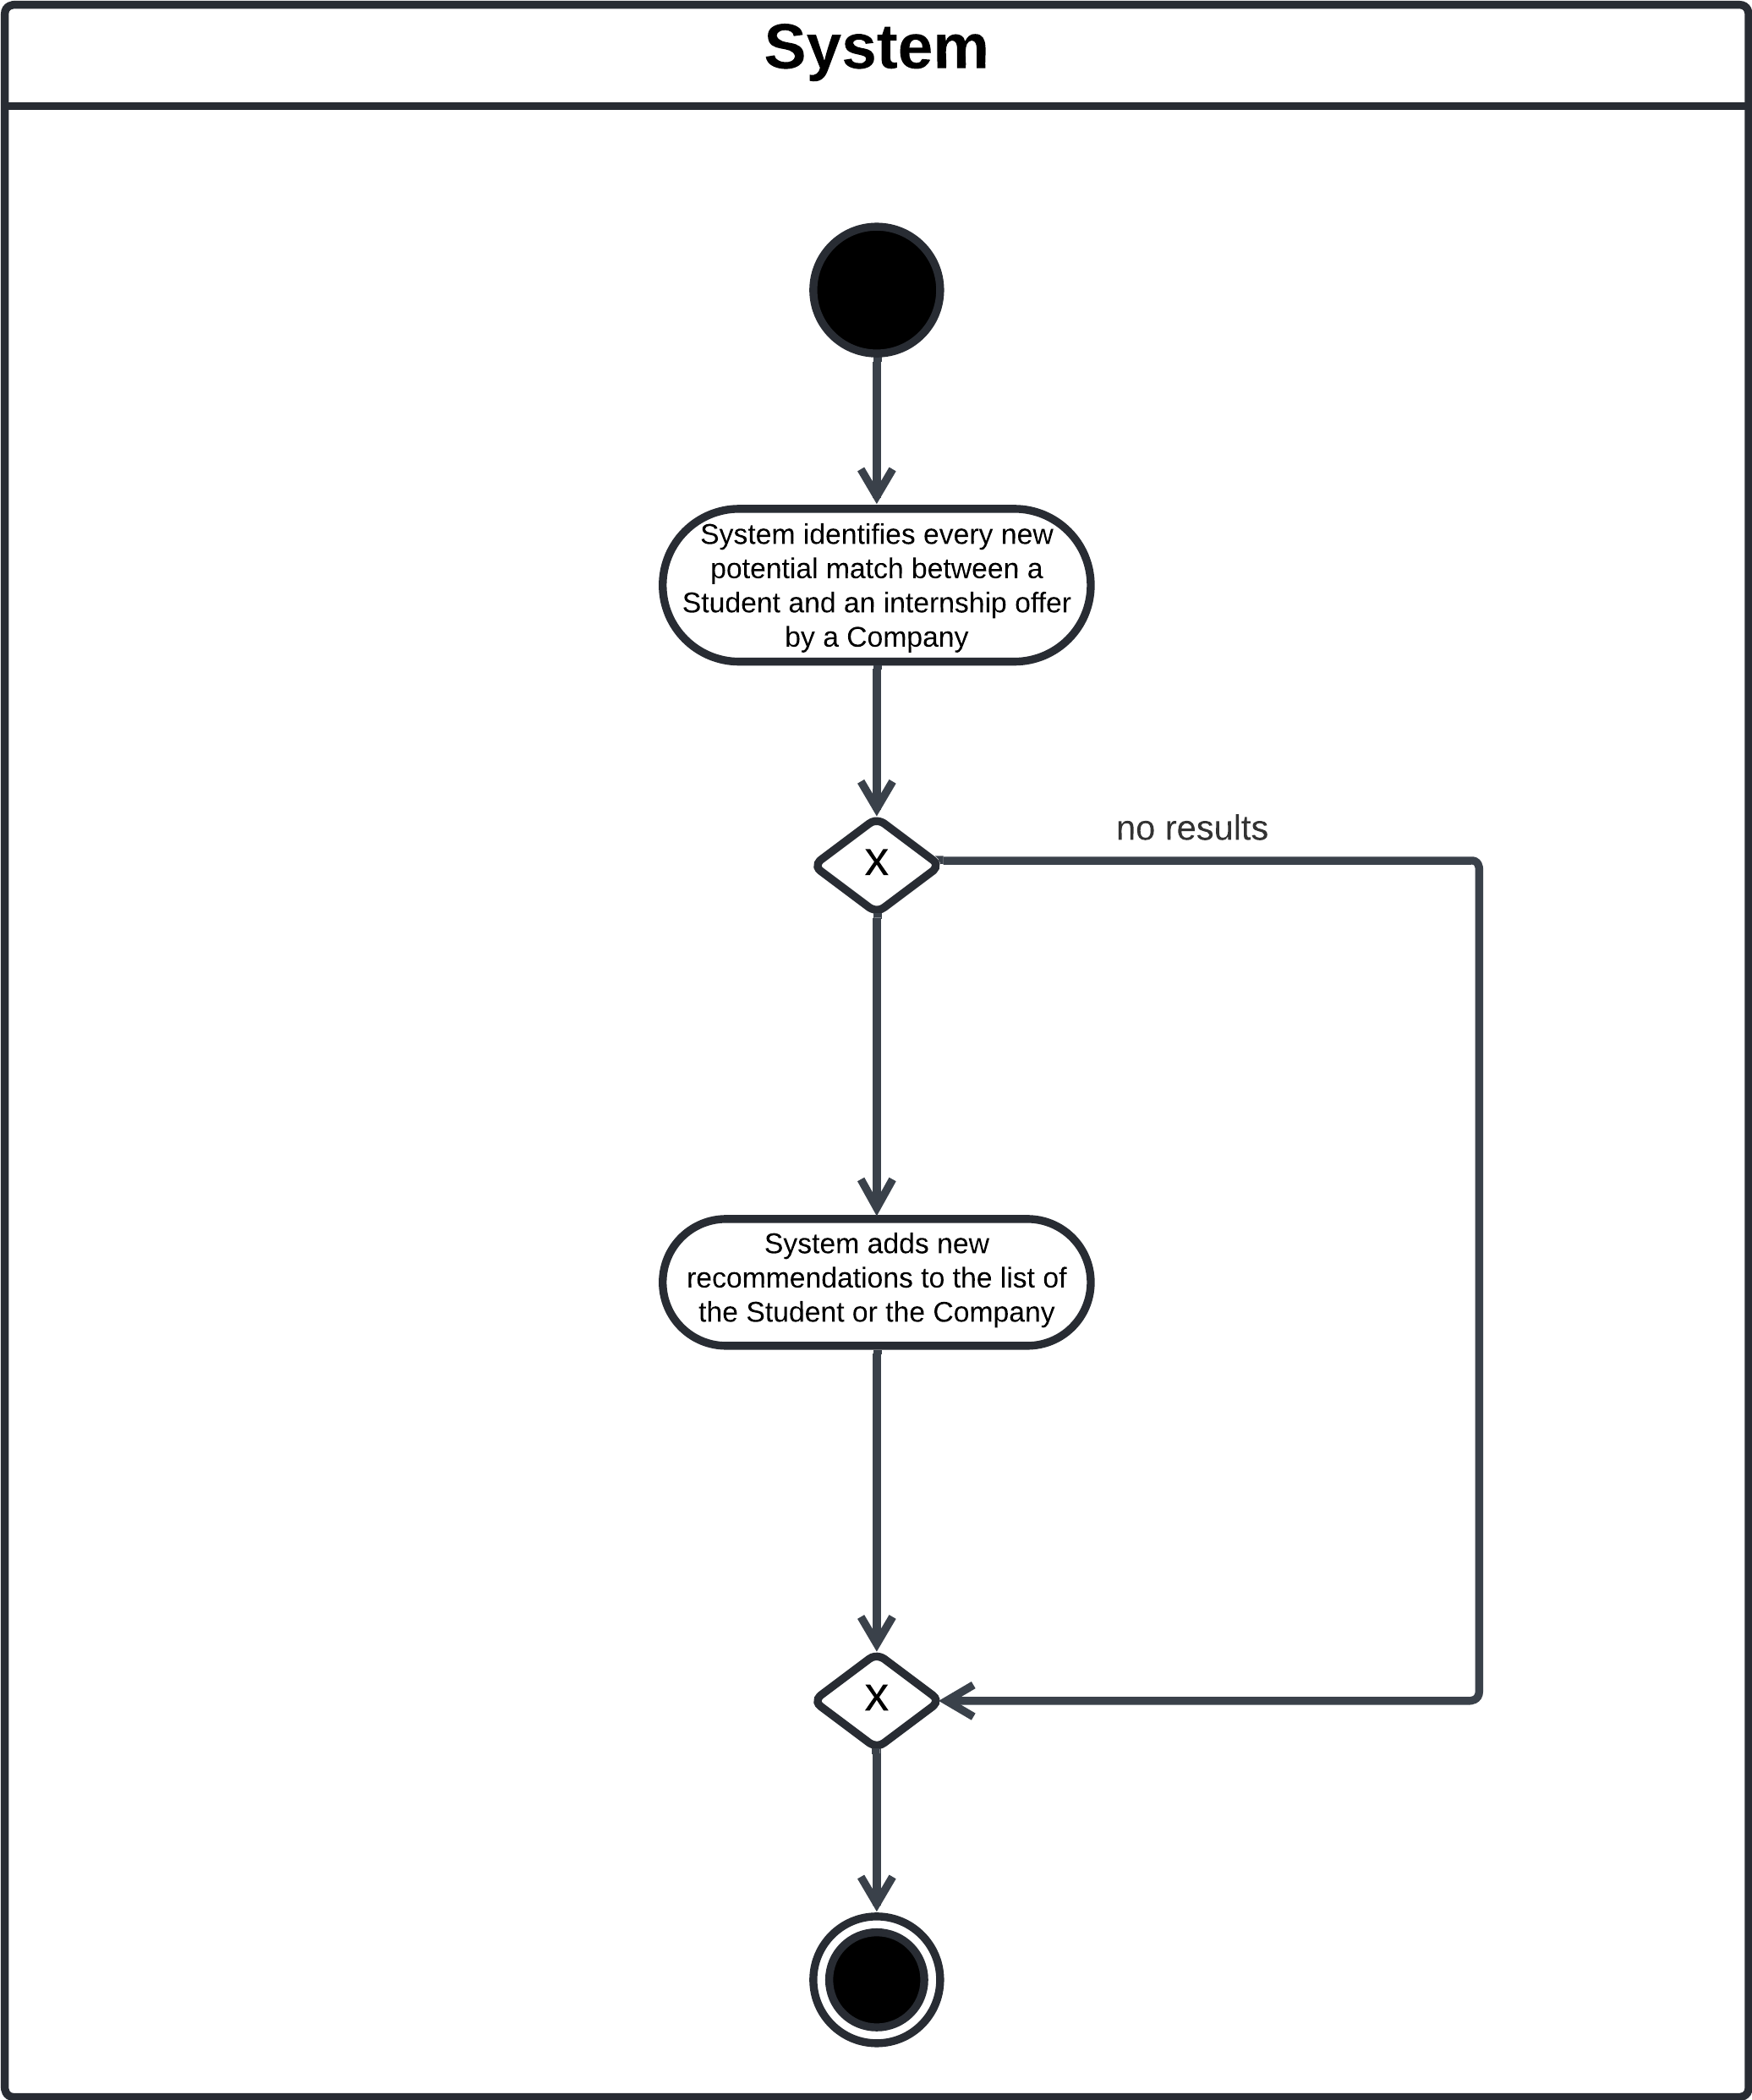
\includegraphics[width=0.9\linewidth]{LaTeXCode/images/activity diagram/UC10.png}
         \caption{Generate Recommendations}
         \label{fig:generate_recommendations_ad}
     \end{center}
\end{figure}

\newpage

\subsubsection*{UC\cuc . Manage Internship Recommendations}
\begin{center}
    \begin{longtable}{|l|p{0.75\linewidth}|}
        \hline
        \textbf{Actor}            & Student \\
        \hline
        \textbf{Entry Conditions} & The Student is logged in and has received at least one recommendation about an internship offer. \\
        \hline
        \textbf{Flow of Events} 
        & \cucsteps. In the dashboard, the Student navigates to the "Manage Recommendations" section. \\
        & \cucsteps. The system displays a list of recommended internship offers for the Student, along with their and the offering Company's information. \\
        & \cucsteps. The Student reviews the list of recommended internship offers, evaluating them. \\
        & \cucsteps. The Student selects a specific recommendation, which expands showing the internship offer details. \\
        & \theucsteps. The student can perform one of the following actions: accept, reject, or postpone the decision. \\
        & \theucsteps.1. If the Student accepts the recommendation, the system automatically performs an "Apply" operation via the \hyperref[subsec: apply_to_internships_uc]{\uline{UC. Apply to an Internship Offer}} to the corresponding internship offer; the system also removes the recommendation from visualization. \\
        & \theucsteps.2. If the Student rejects the recommendation, the latter is simply removed from visualization by the system. \\
        & \cucsteps.3. If the Student chooses to postpone the decision, the system doesn't perform any operation.\\
        & \cucsteps. The Student may repeat this process until there are no pending recommendations.\\
        \hline
        \textbf{Exit Conditions}   & The decision on the selected recommendations is recorded, and the internship offers' statuses are updated accordingly in the system. \\
        \hline
        \textbf{Exceptions}       & None \\
        \hline
    \end{longtable}
\end{center}

\begin{figure}[H]
    \begin{center}
         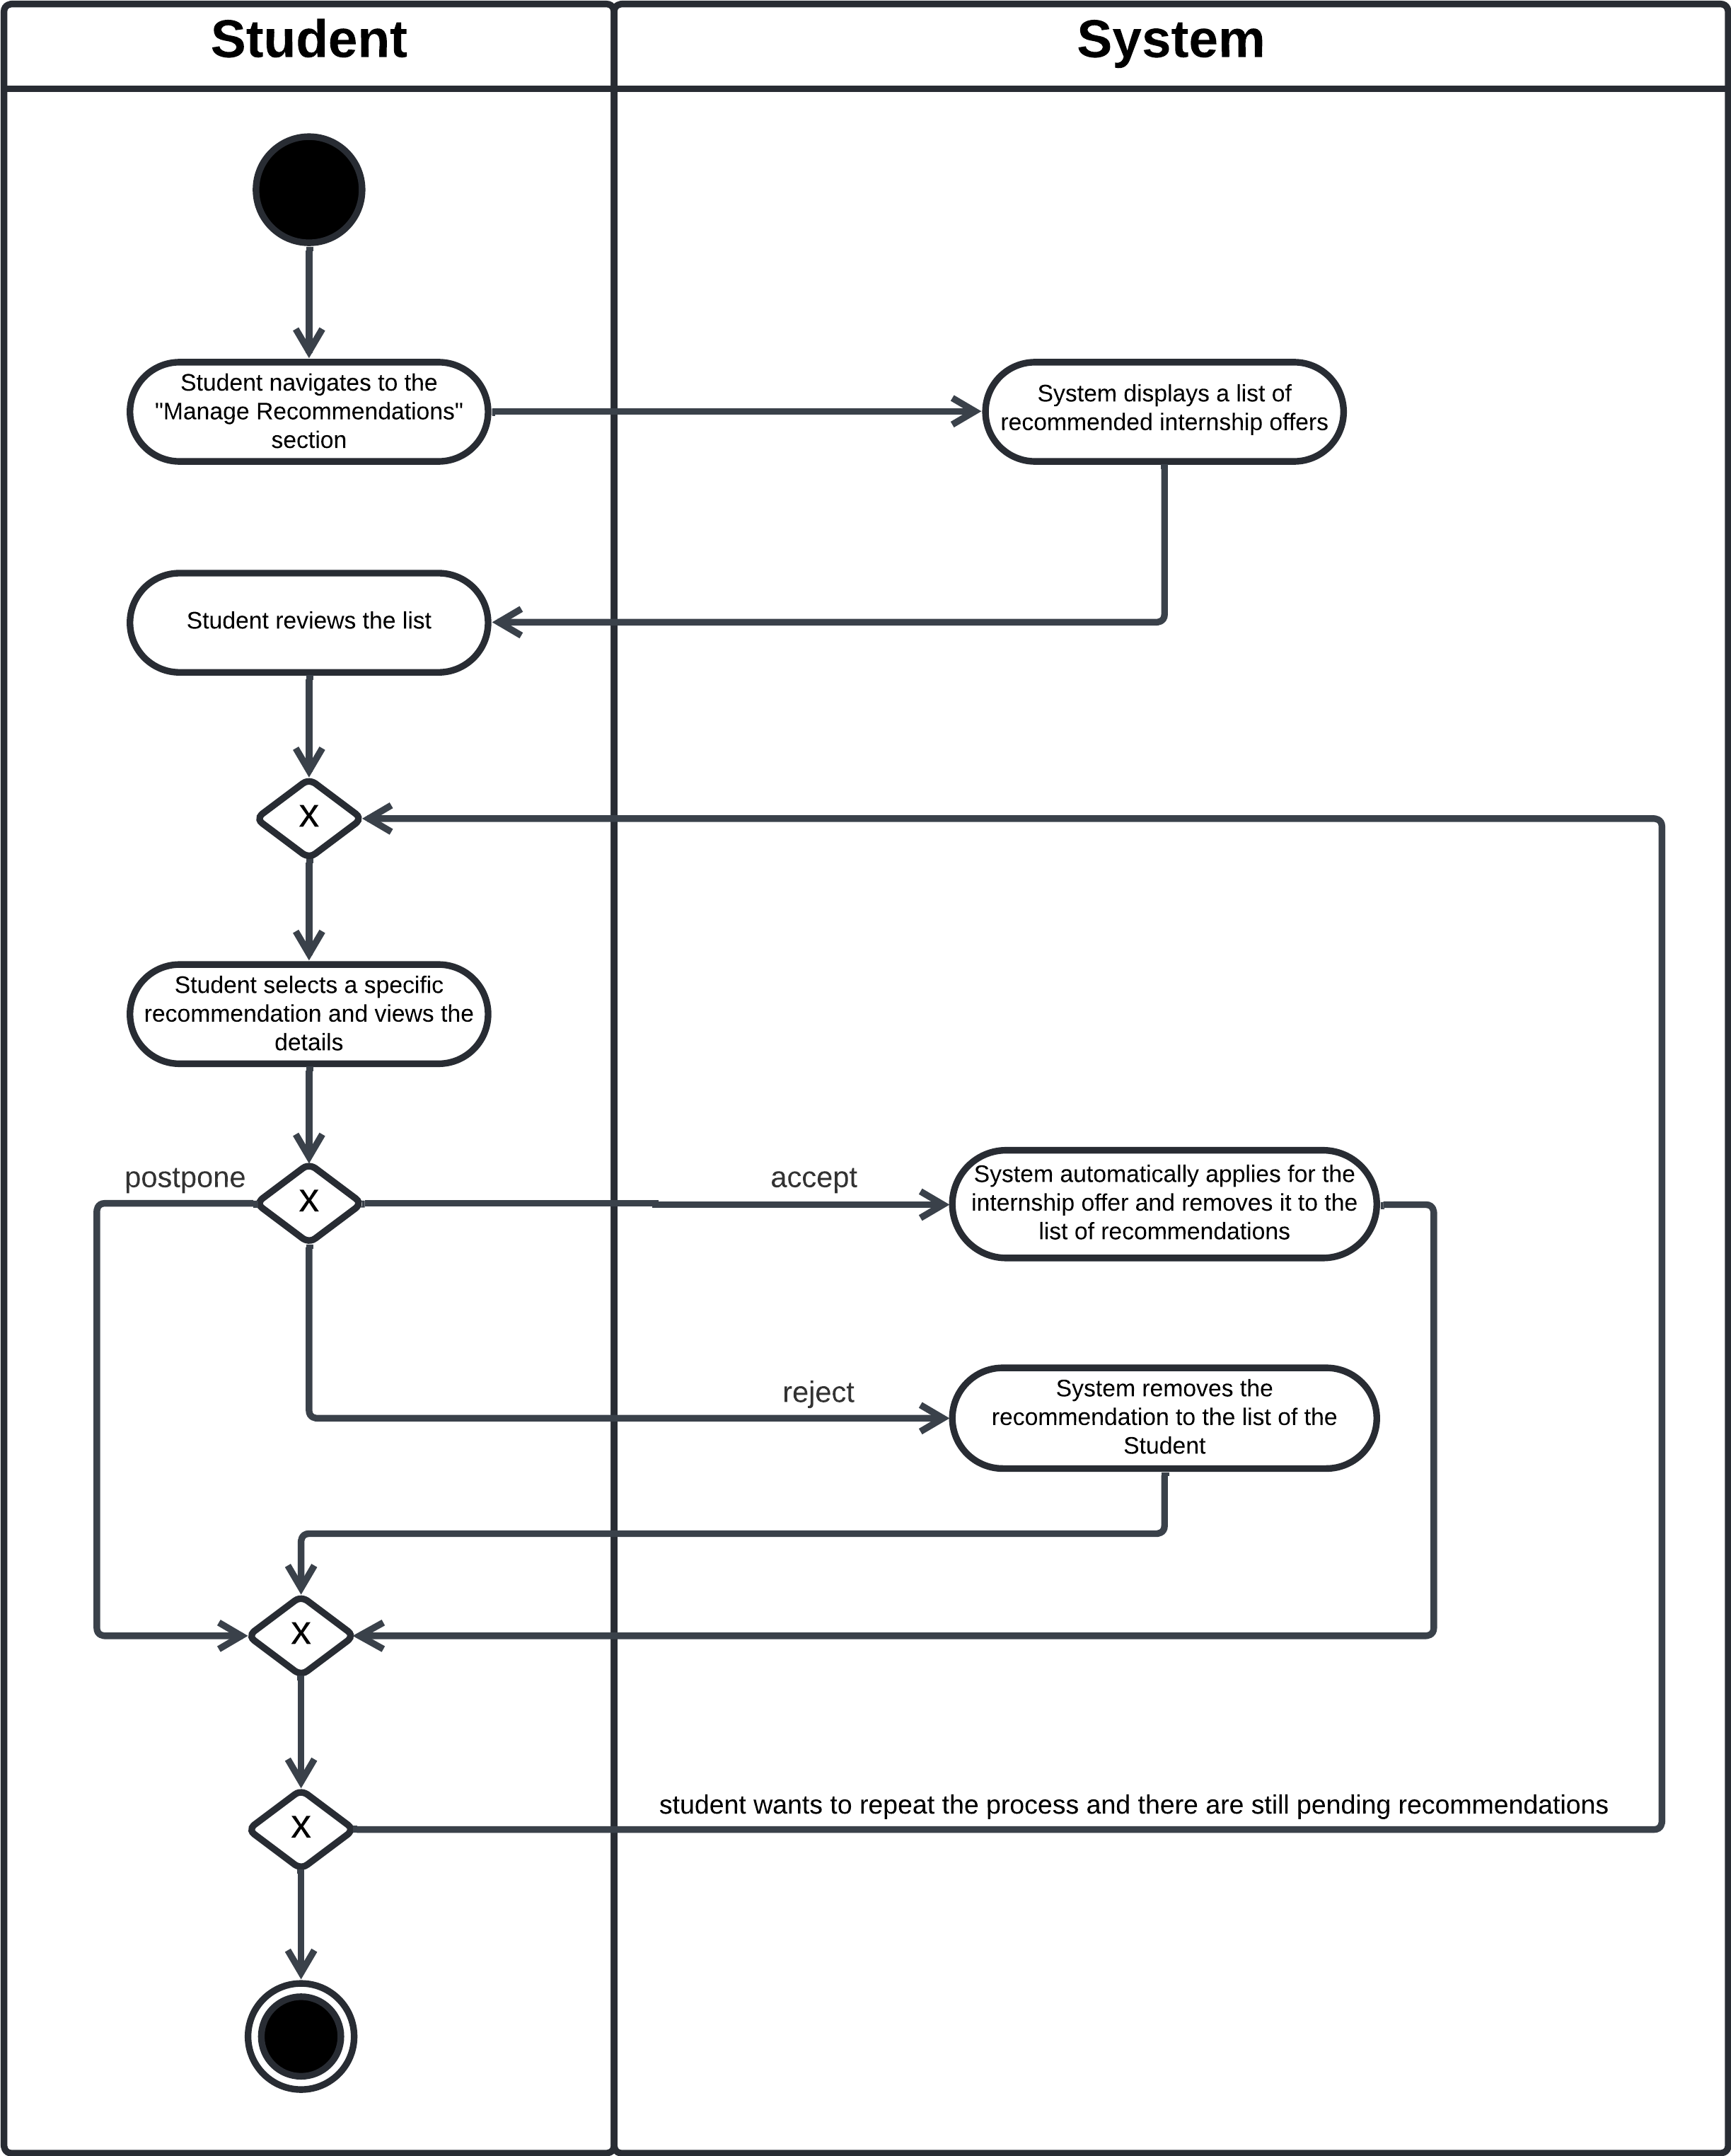
\includegraphics[width=1\linewidth]{LaTeXCode/images/activity diagram/UC11.png}
         \caption{Manage Internship Recommendations}
         \label{fig:manage_internship_recommendations_ad}
     \end{center}
\end{figure}

\newpage

\subsubsection*{UC\cuc . Manage Students Recommendations}
\begin{center}
    \begin{longtable}{|l|p{0.75\linewidth}|}
        \hline
        \textbf{Actor}            & Company \\
        \hline
        \textbf{Entry Conditions} & The Company is logged in and has received at least one recommendation about a Student for any of their internship offers. \\
        \hline
        \textbf{Flow of Events} 
        & \cucsteps. In the dashboard, the Company navigates to the "Manage Recommendations" section. \\
        & \cucsteps. The system displays a list of recommended students for the available internship offers, along with their profile information. \\
        & \cucsteps. The Company reviews the list of recommended students, evaluating them. \\
        & \cucsteps. The Company selects a specific recommendation, which expands showing the student's profile. \\
        & \theucsteps. The Company can perform one of the following actions: accept, reject, or postpone the decision.\\
        & \theucsteps.1. If the Company accepts the recommendation, the system marks it as "Selected" and the corresponding Student receives a dual recommendation, on which they will be able to decide; the system also removes the recommendation from visualization. \\
        & \theucsteps.2. If the Company rejects the recommendation, the latter is simply removed from visualization by the system. \\
        & \cucsteps.3. If the Company chooses to postpone the decision, the system doesn't perform any operation.\\
        & \cucsteps. The Company may repeat this process until there are no pending recommendations.\\
        \hline
        \textbf{Exit Conditions}   & The decision on the selected recommendations is recorded, and the students' statuses are updated accordingly in the system. \\
        \hline
        \textbf{Exceptions}       & None \\
        \hline
    \end{longtable}
\end{center}

\begin{figure}[H]
    \begin{center}
         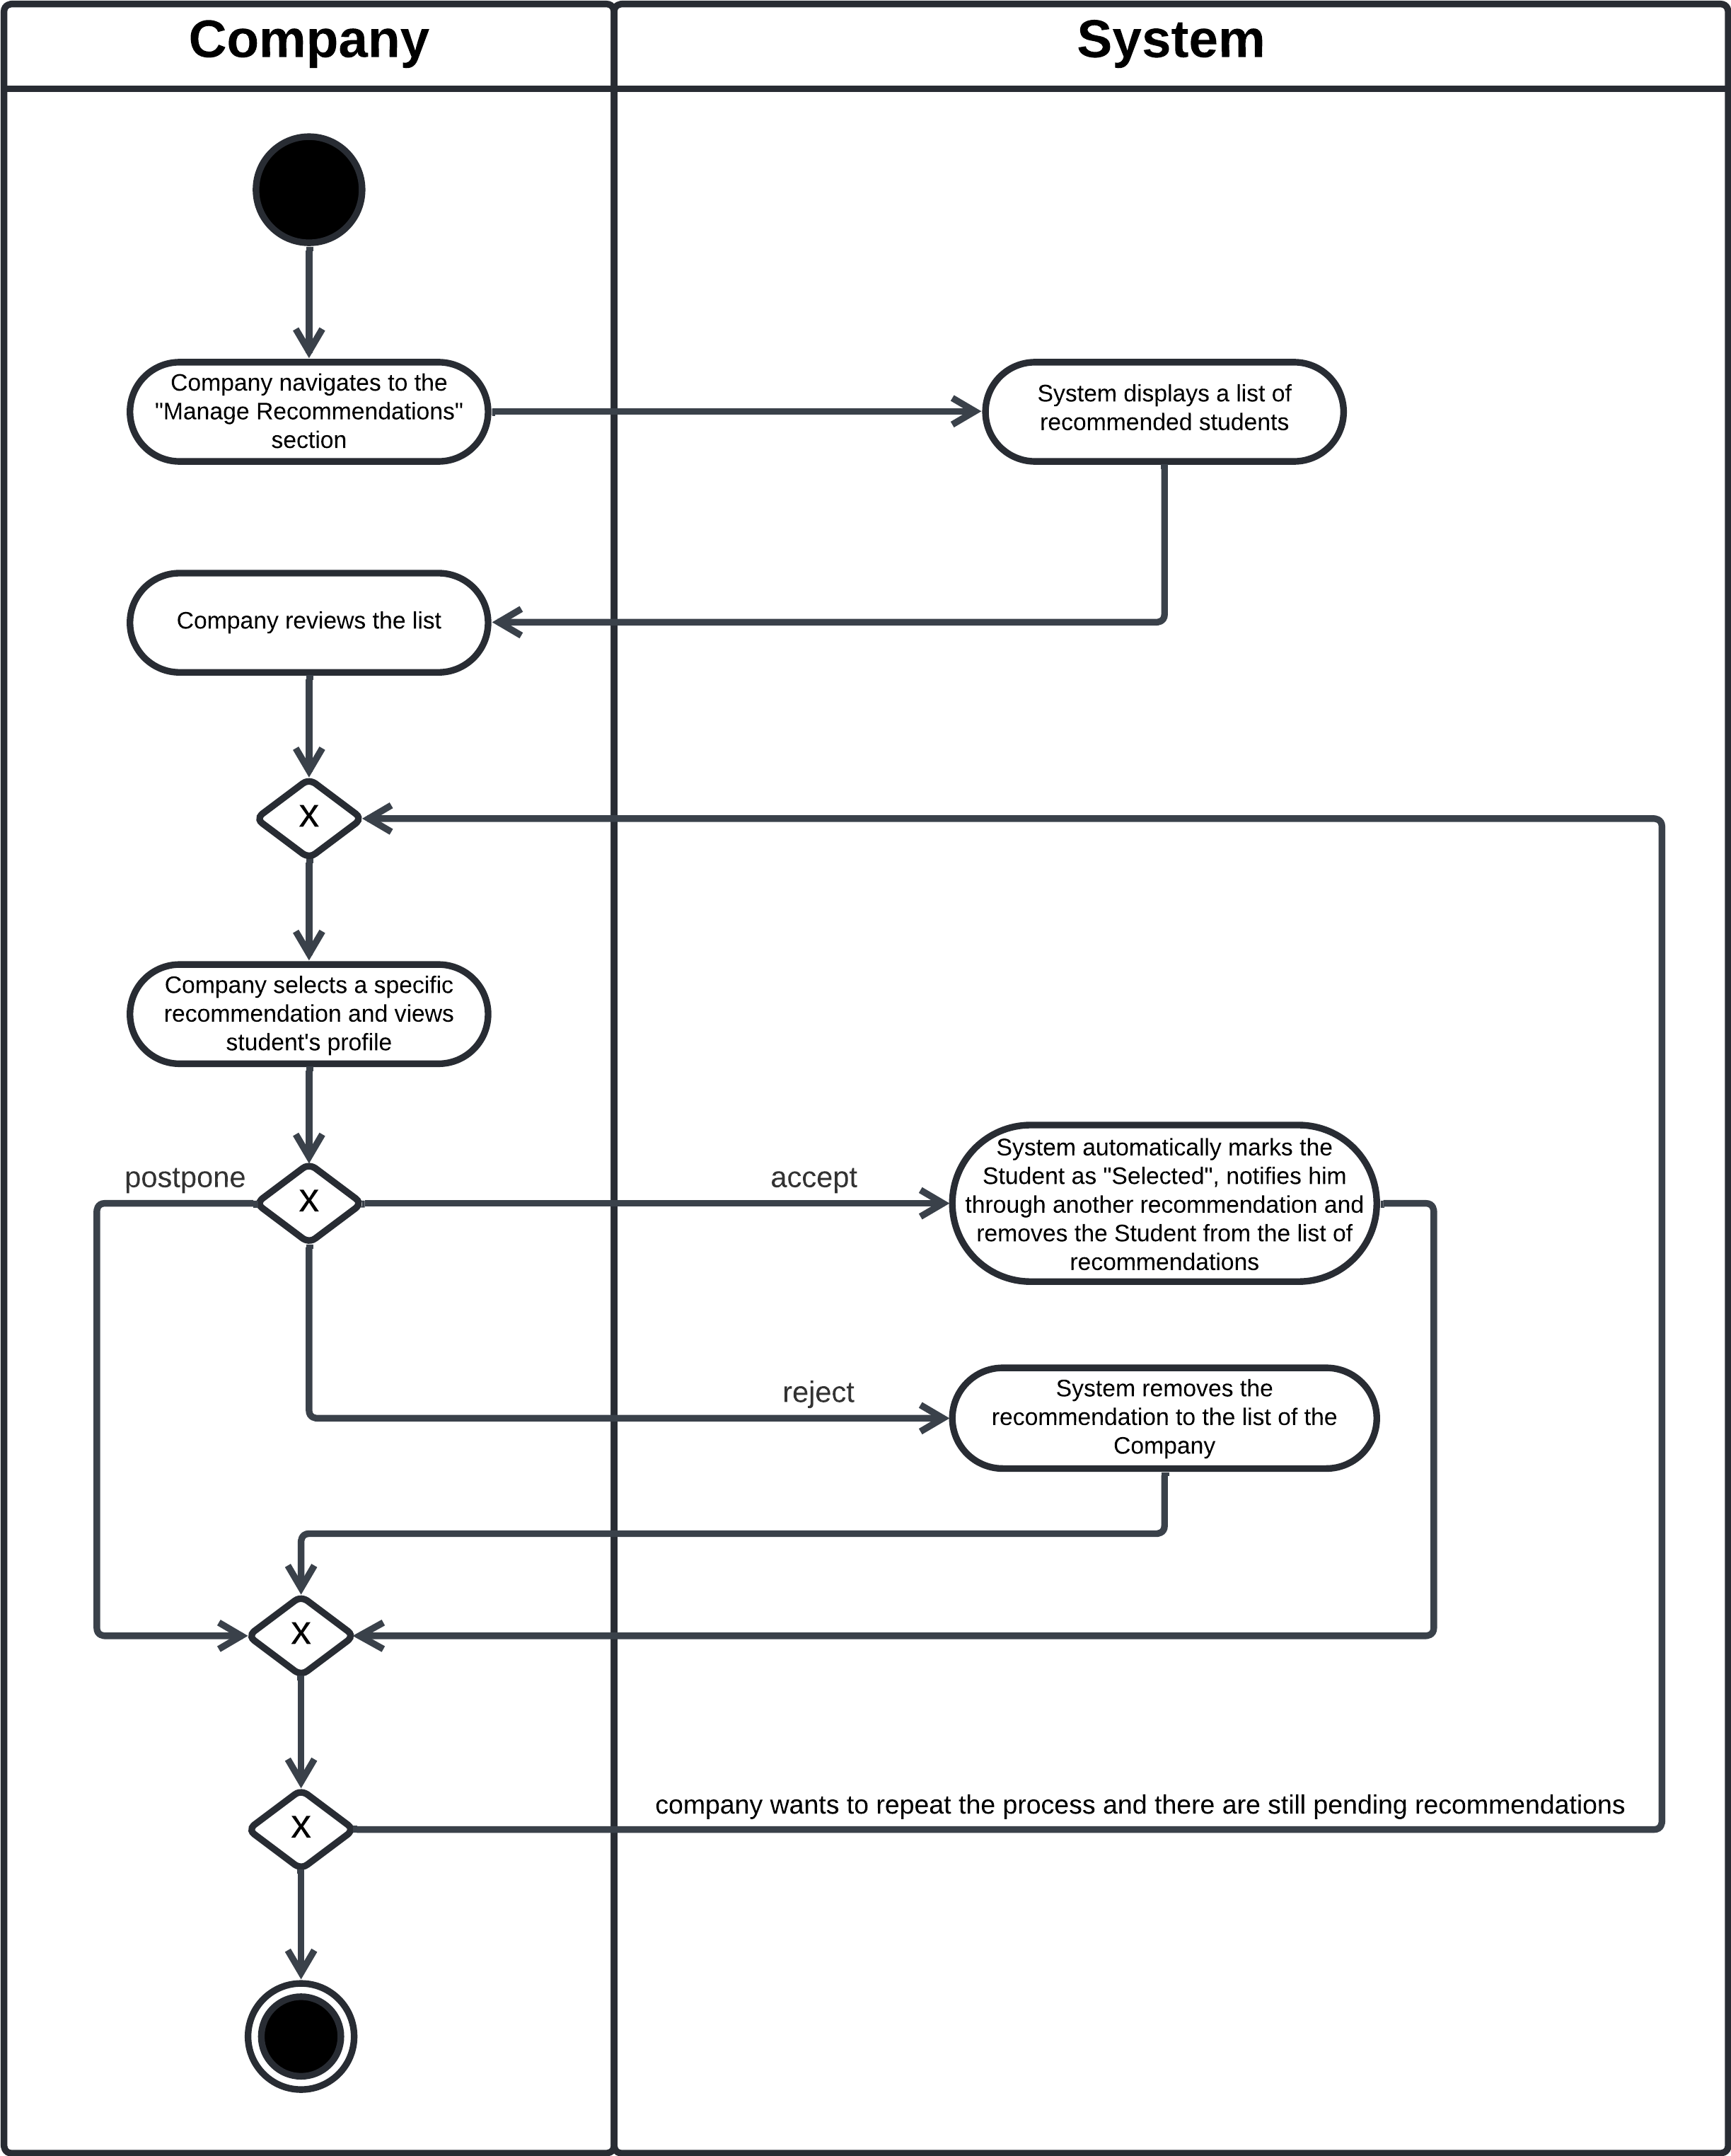
\includegraphics[width=1\linewidth]{LaTeXCode/images/activity diagram/UC12.png}
         \caption{Manage Students Recommendations}
         \label{fig:manage_students_recommendations_ad}
     \end{center}
\end{figure}

\newpage

\subsubsection*{UC\cuc . Manage an Interview}
\begin{center}
    \begin{longtable}{|l|p{0.75\linewidth}|}
        \hline
        \textbf{Actor}            & Company, Student\\
        \hline
        \textbf{Entry Conditions} & The application deadline for a specific internship offer has expired and the Company has accepted at least one application to that offer, establishing a contact with the accepted Student.\\
        \hline
        \textbf{Flow of Events}       
        & \cucsteps. From the dashboard page, the Company navigates to the page of one of its internship offers.\\
        & \cucsteps. On the internship offer page, the Company selects a Student from the list of candidates for that offer, opening a new page to arrange the interview. \\ 
        & \cucsteps. The Company creates an interview invitation to the Student, specifying the date, time, format (in-platform or in-person) and an optional text description with more details. \\
        & \cucsteps. The Company reviews and forwards the interview invitation by confirming its information through the "Confirm" button. \\
        & \cucsteps. The Student receives the invitation to the interview on the corresponding section of its dashboard page and navigates to the platform to review the invitation details. \\
        & \theucsteps. The Student accepts or declines the interview invitation, confirming their preference. If declining, he is able to provide a reason behind the choice, so that the Company may reschedule the interview.\\
        & \theucsteps.1. If the Student accepts the invitation, the interview is conducted according to the specified details, enabling the Company to assess the student's suitability for the internship either by sharing multiple questions through the platform or by interviewing the candidate in person and later recording the results on the system.\\
        & \cucsteps.2. If the Student declines the invitation, the system marks the interview as declined. The Company sees the rejection and can decide whether to reschedule based on the given reason. \\
        & \cucsteps. After the interview, the Company provides an evaluation of the student’s performance, inserting strengths, weaknesses, and suitability for the role, and submits the results through the platform.\\
        & \cucsteps. The system records the evaluation and updates the student’s status in the selection process: "Interview Completed", "Selected" or "Rejected". \\
        \hline
        \textbf{Exit Conditions}   & The interview is completed, and the Student’s status in the selection process is updated in the system, becoming available for consulting. \\       
        \hline
        \textbf{Exceptions}       & None \\
        \hline
    \end{longtable}
\end{center}

\begin{figure}[H]
    \begin{center}
         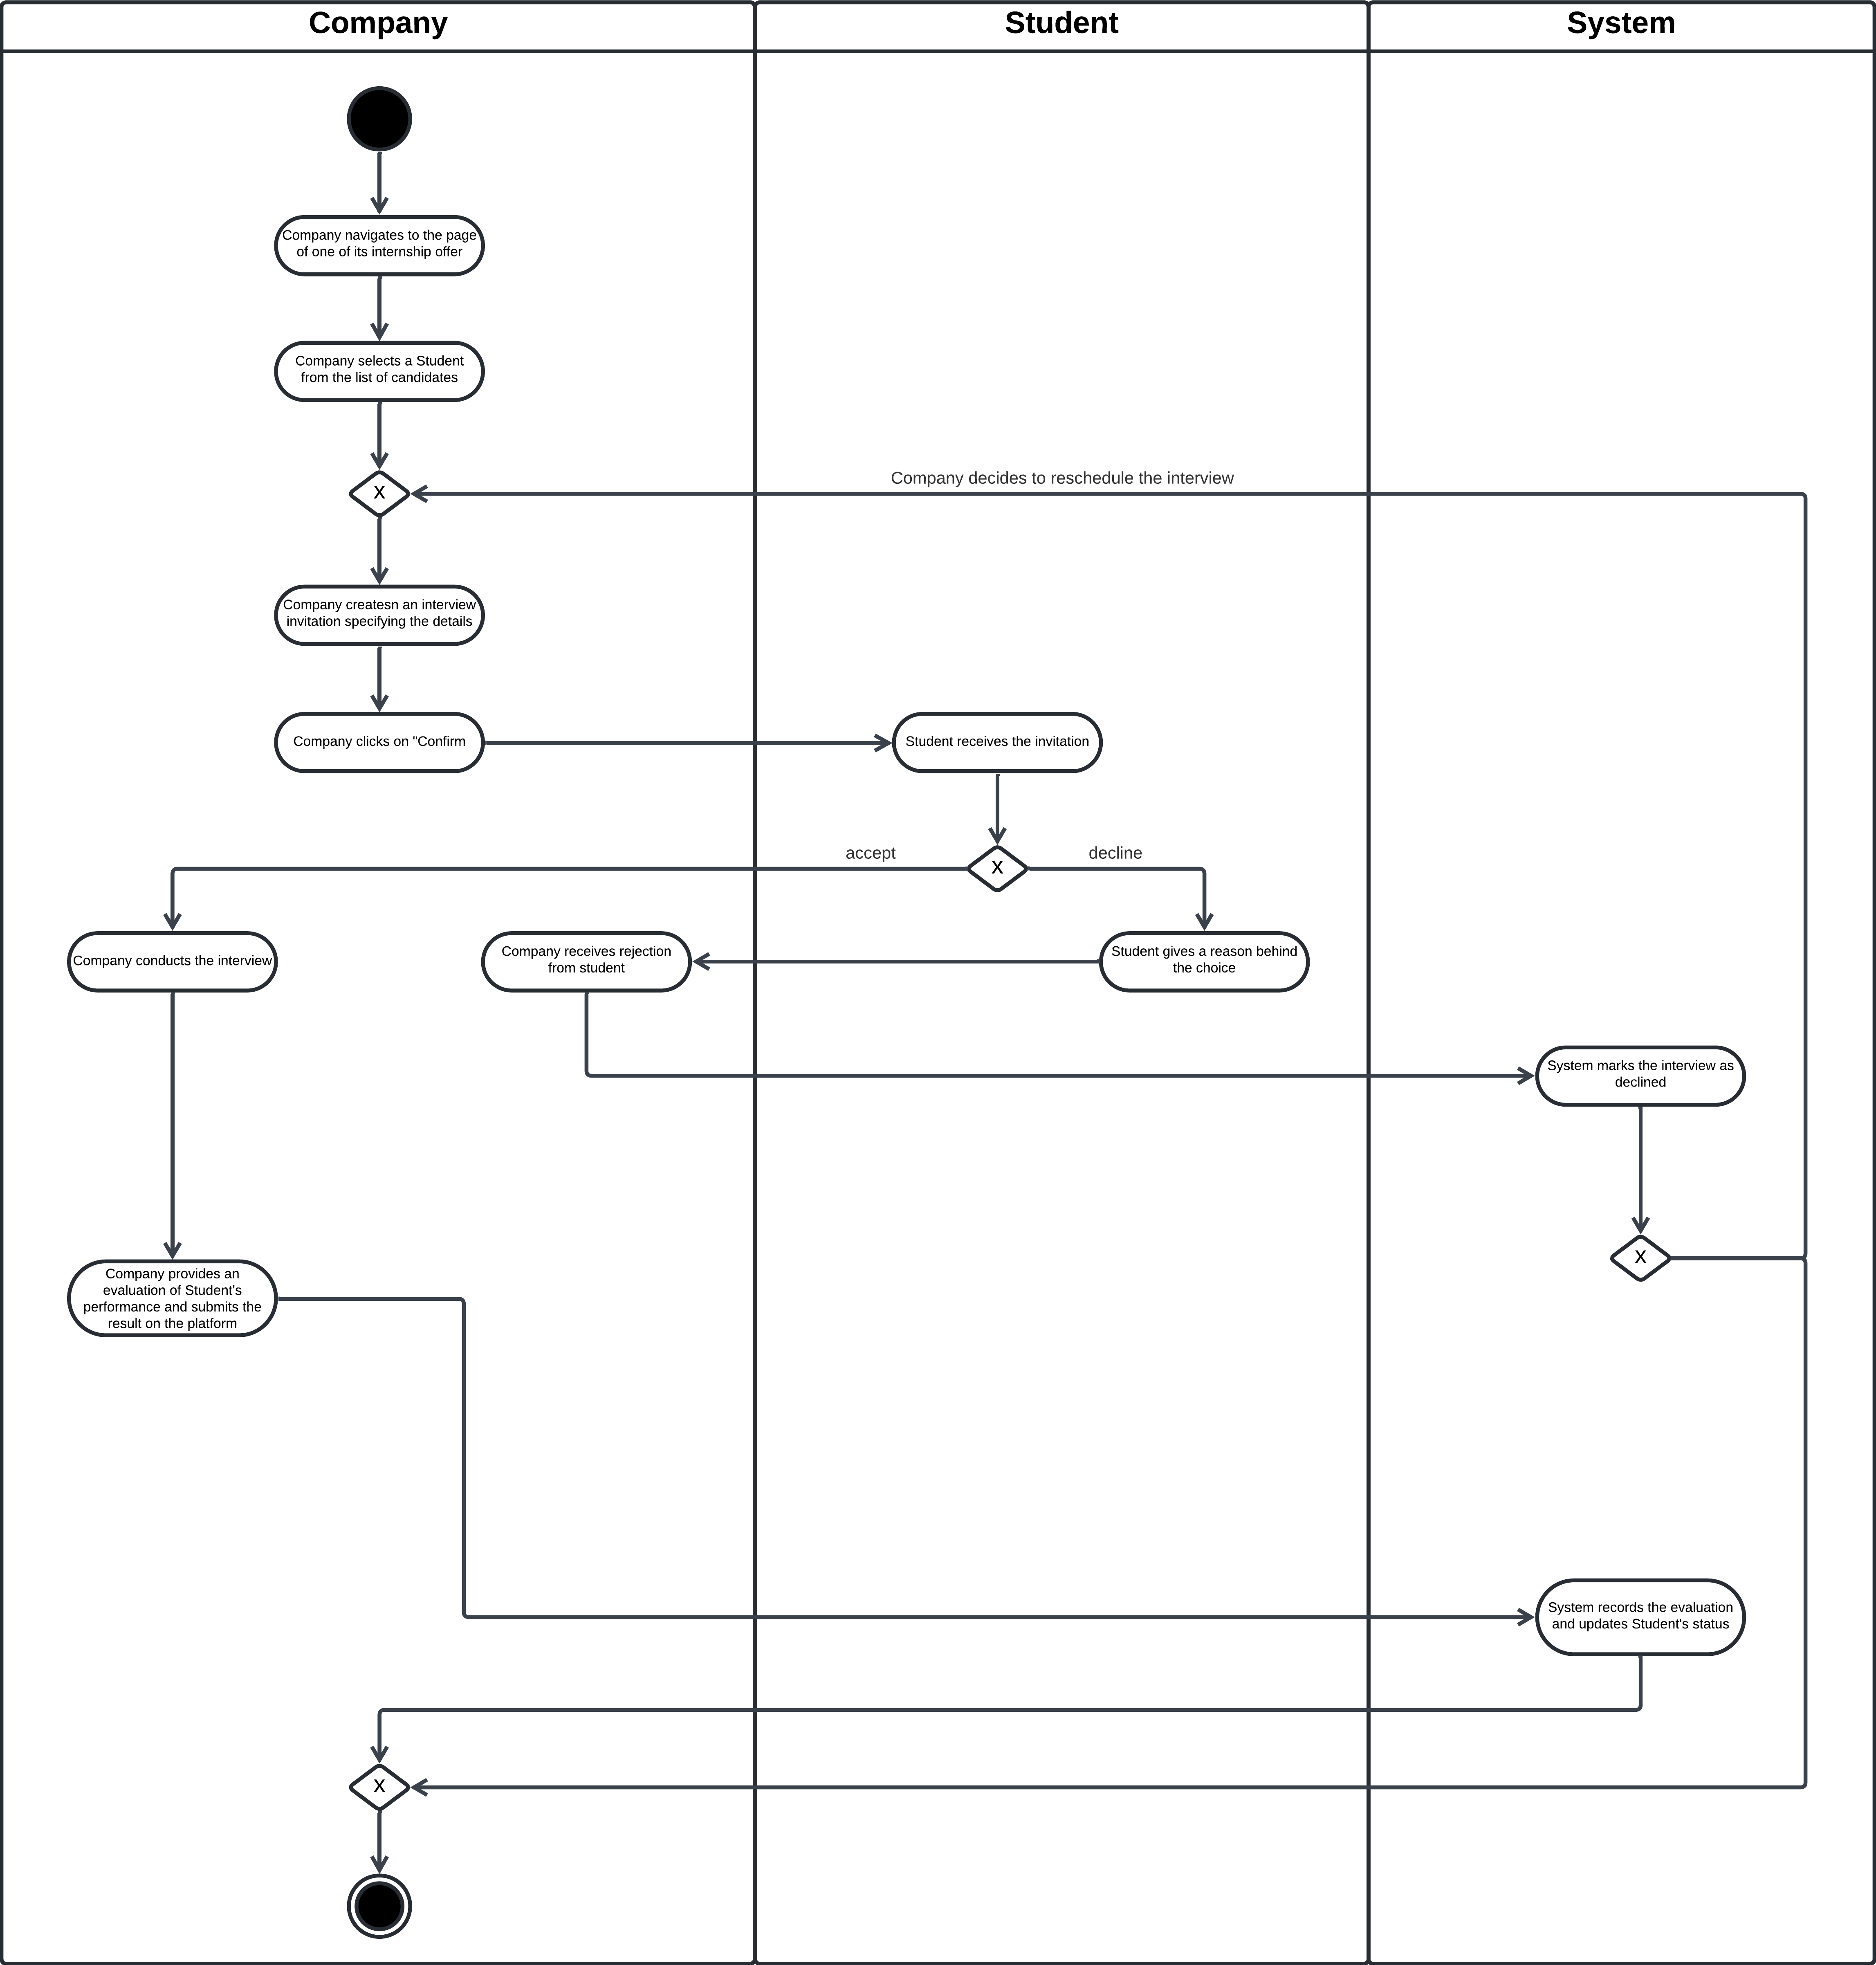
\includegraphics[width=1\linewidth]{LaTeXCode/images/activity diagram/UC13.png}
         \caption{Manage an Interview}
         \label{fig:manage_interview_ad}
     \end{center}
\end{figure}

\newpage

\subsubsection*{UC\cuc . Provide Information for an ongoing Internship}
\begin{center}
    \begin{longtable}{|l|p{0.75\linewidth}|}
        \hline
        \textbf{Actor}            & Party (Student or Company)\\
        \hline
        \textbf{Entry Conditions} & The Party is logged into the S\&C platform, is actively involved in the selected ongoing internship and has identified new information about it to be provided.\\
        \hline
        \textbf{Flow of Events}   
        & \cucsteps. On the ongoing internship's page, the Party clicks the "Post information" button. \\ 
        & \cucsteps. The Party provides new information about the selected ongoing internship in the given text field. \\
        & \cucsteps. The Party confirms the information provided by clicking the confirmation button. \\
        & \cucsteps. The system records the new information inserted and posts it on the ongoing internship's page. \\
        \hline
        \textbf{Exit Conditions}   & The ongoing internship's page is updated and those changes are recorded in the system. \\    
        \hline
        \textbf{Exceptions}       & \begin{itemize}
            \item The Party closes the page without completing the process: the system doesn't record any information and displays the Party's dashboard.
        \end{itemize} \\
        \hline 
    \end{longtable}
\end{center}
\label{subsec: provide_information_ongoing_uc}

\begin{figure}[H]
    \begin{center}
         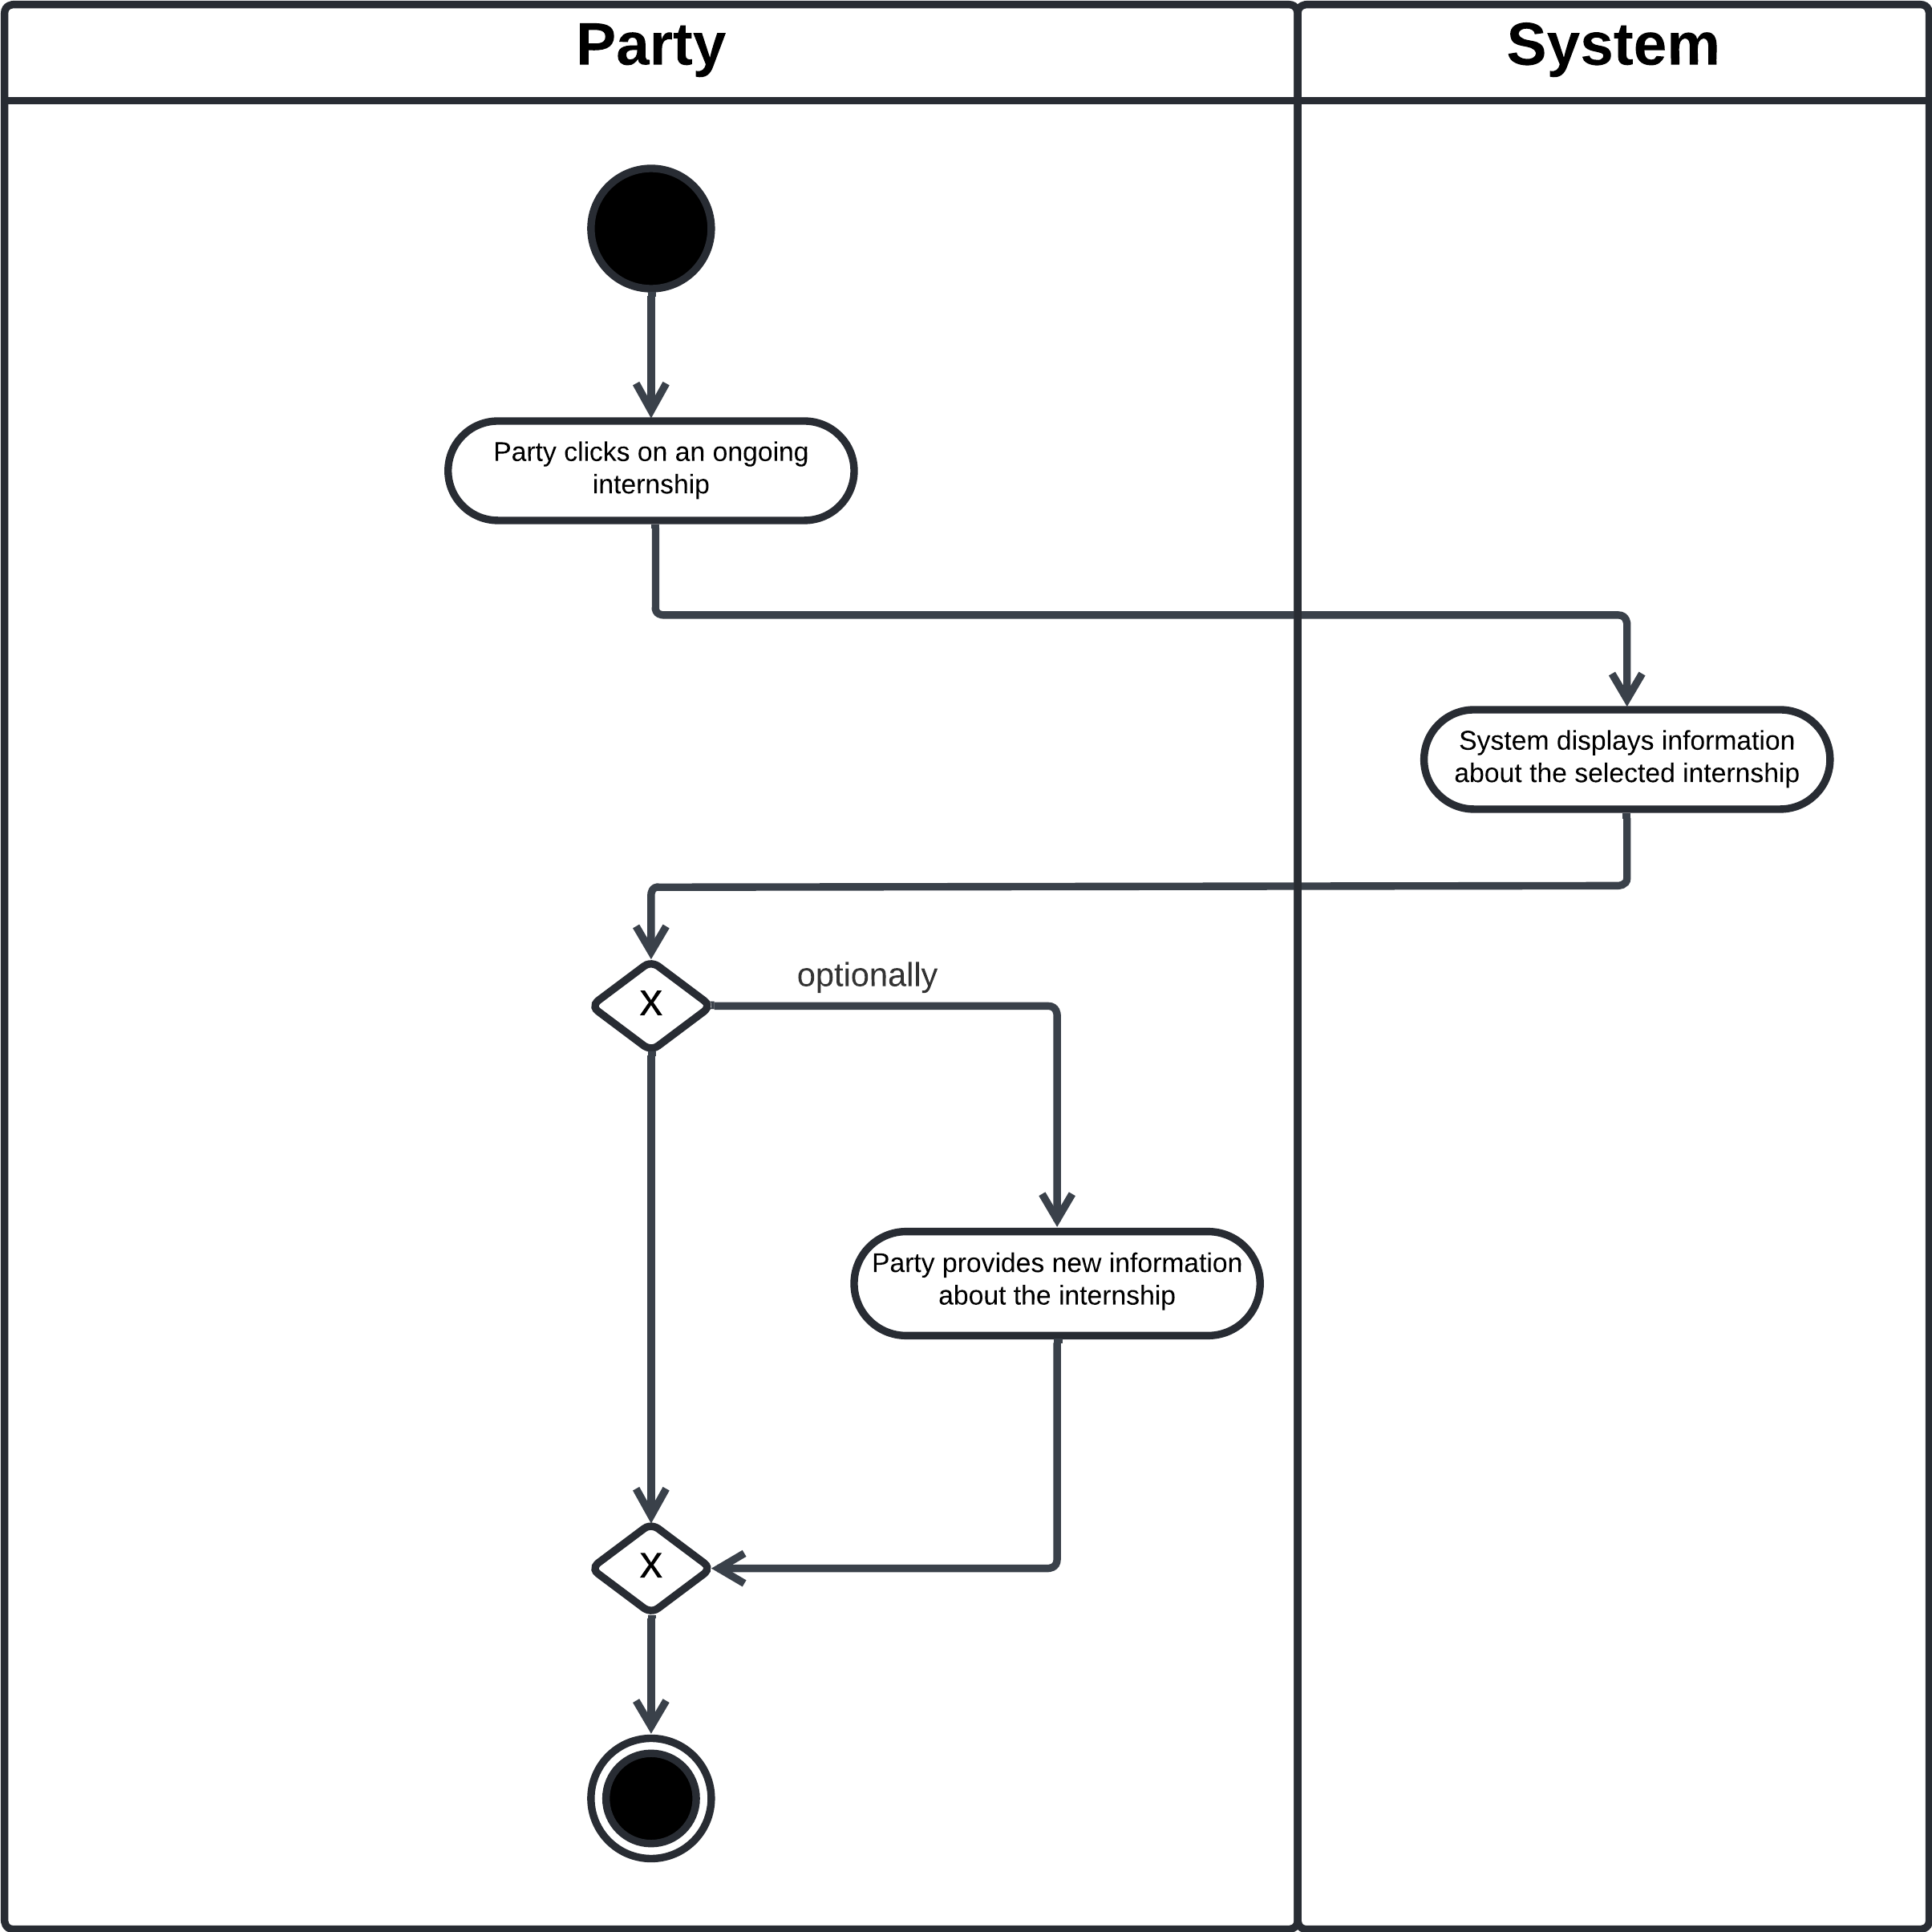
\includegraphics[width=1\linewidth]{LaTeXCode/images/activity diagram/UC15.png}
         \caption{Provide Information for an ongoing Internship}
         \label{fig:provide_information_ongoing_ad}%
     \end{center}
\end{figure}

\newpage

\subsubsection*{UC\cuc . Monitor an ongoing Internship}
\begin{center}
    \begin{longtable}{|l|p{0.75\linewidth}|}
        \hline
        \textbf{Actor}            & Party \\
        \hline
        \textbf{Entry Conditions} & The Party is logged into the S\&C platform and is actively involved in at least an ongoing internship. \\
        \hline
        \textbf{Flow of Events}       
        & \cucsteps. In the dashboard, the Party clicks on an ongoing internship offer in which it is actively participating, entering that internship's page. \\
        & \cucsteps. The system displays all the information about the selected internship. \\
        & \cucsteps. Optionally, the Party provides new information about the internship offer via the \hyperref[subsec: provide_information_ongoing_uc]{\uline{UC. Provide Information for an ongoing Internship}} functionality. \\
        \hline
        \textbf{Exit Conditions}   & The system displays all the information about the selected ongoing internship. \\
        \hline
        \textbf{Exceptions}       & None \\
        \hline
    \end{longtable}
\end{center}

\begin{figure}[H]
    \begin{center}
         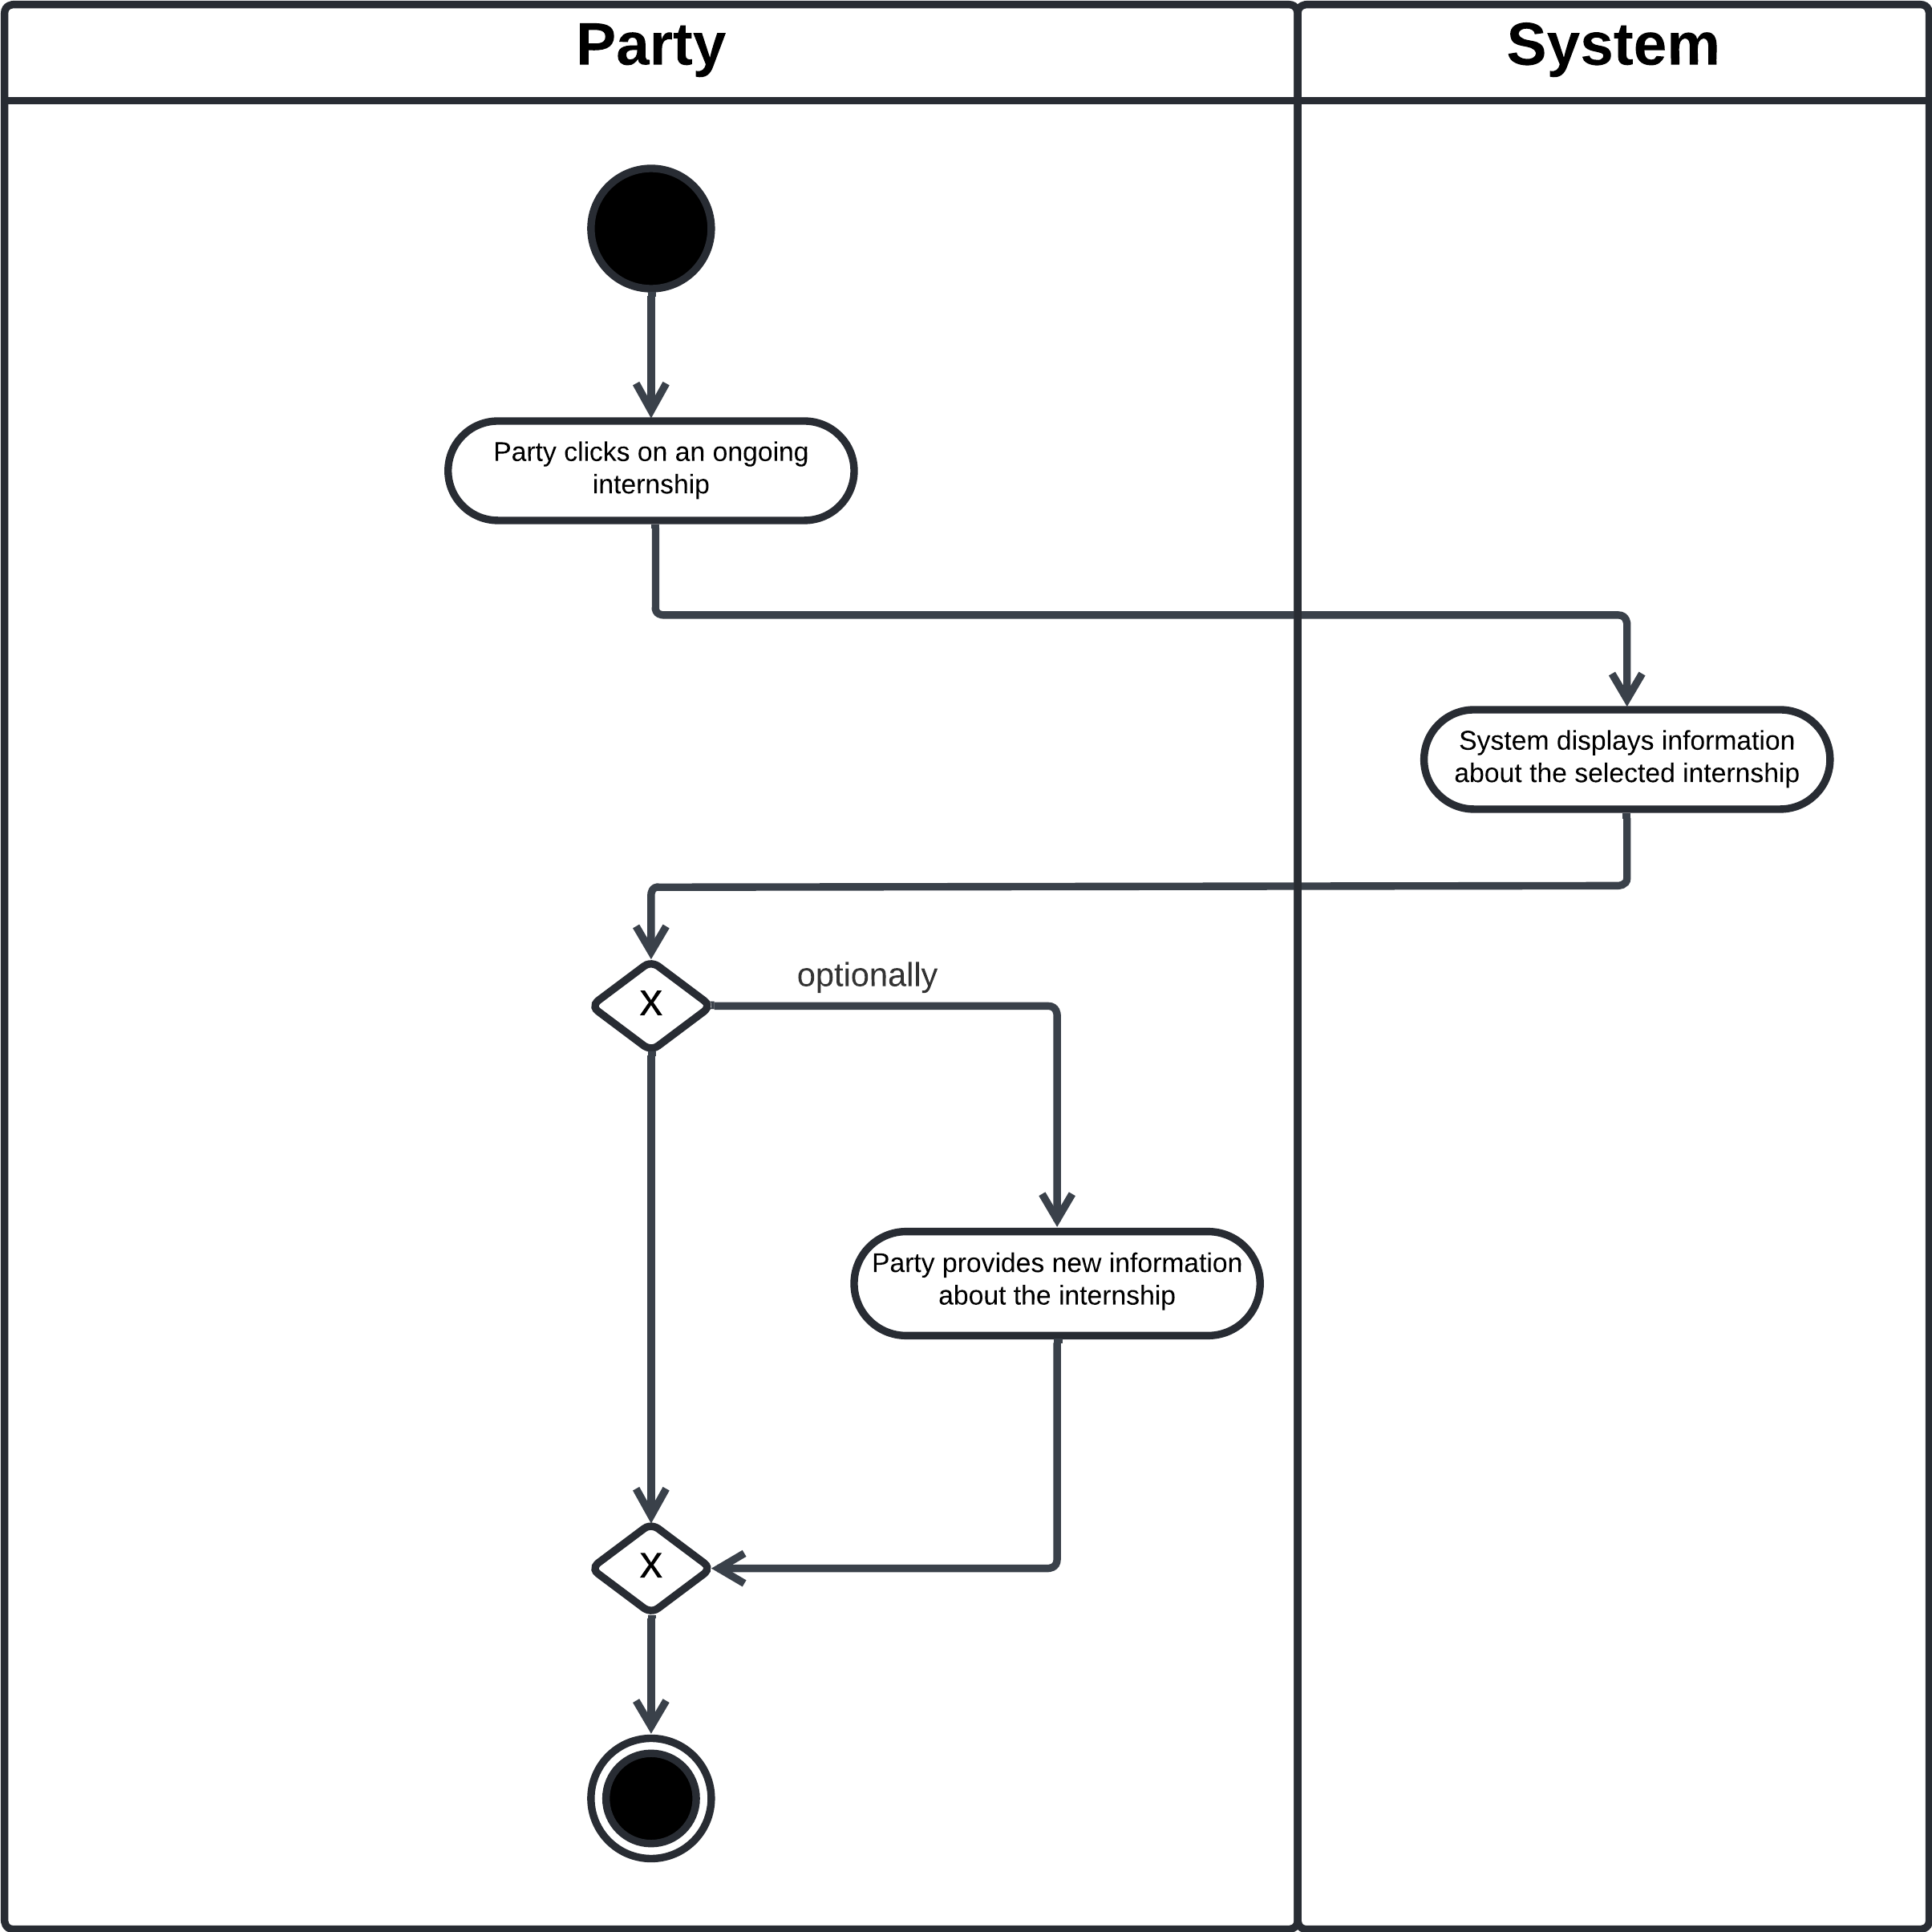
\includegraphics[width=1\linewidth]{LaTeXCode/images/activity diagram/UC15.png}
         \caption{Monitor an ongoing Internship}
         \label{fig:monitor_internship_ad}%
     \end{center}
\end{figure}

\newpage

\subsubsection*{UC\cuc . Report Problems during an Internship}
\begin{center}
    \begin{longtable}{|l|p{0.75\linewidth}|}
        \hline
        \textbf{Actor}            & Party (Student or Company) \\
        \hline
        \textbf{Entry Conditions} & The Party is logged into the S\&C platform, is actively involved in an internship and has identified an issue requiring intervention. \\
        \hline
        \textbf{Flow of Events}       
        & \cucsteps. In the dashboard, the Party navigates to the "Report Problems" section.\\ 
        & \cucsteps. The Party provides a detailed description of the issue, providing:
        \begin{itemize}
            \item Nature of the problem.
            \item Relevant details about when and how the issue occurred.
            \item Optionally, attachments as images or documents to further describe the problem.
        \end{itemize} \\
        & \cucsteps. The Party submits the problem report by clicking the "Report" button.\\ 
        & \cucsteps. The system forwards the Party's report to the Student's University. \\ 
        \hline
        \textbf{Exit Conditions}   & The issue reported by the Party is registered in the system and made available to the University. \\       
        \hline
        \textbf{Exceptions}       & \begin{itemize}
            \item Some mandatory fields are missing: the system doesn't allow the Party to complete the procedure until all the mandatory fields are filled out.
        \end{itemize} \\
        \hline
    \end{longtable}
\end{center}

\begin{figure}[H]
    \begin{center}
         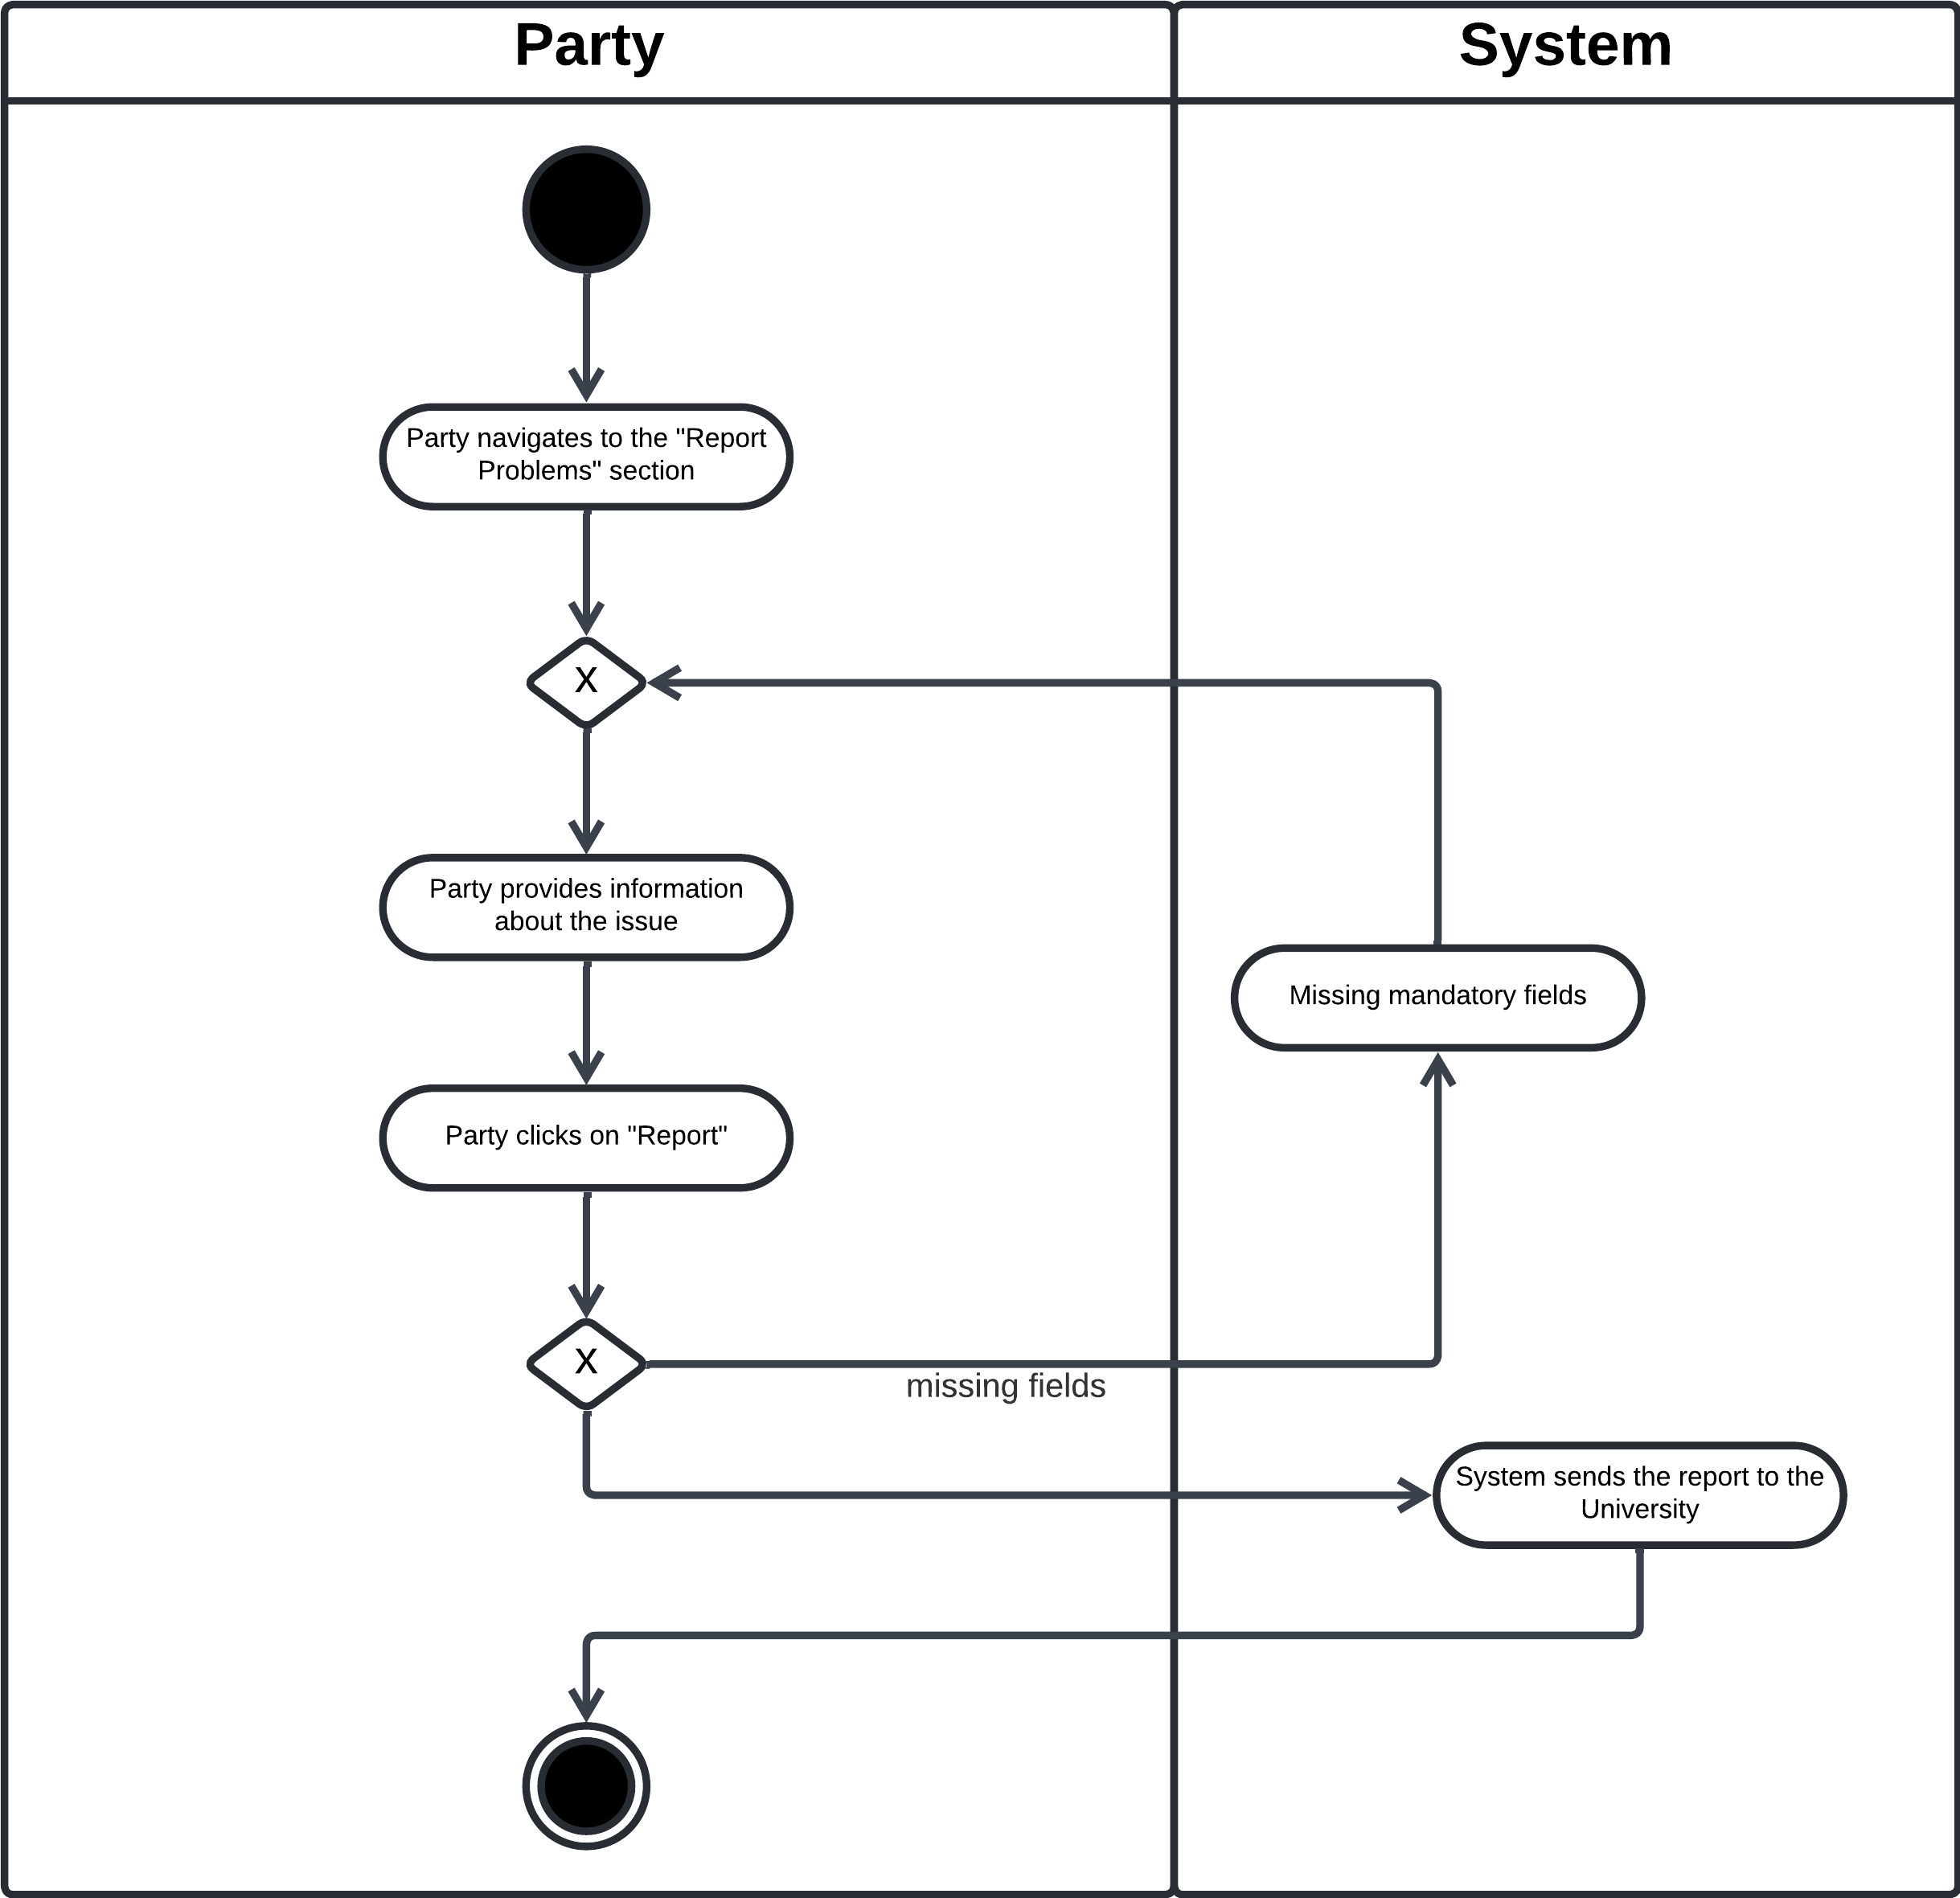
\includegraphics[width=1\linewidth]{LaTeXCode/images/activity diagram/UC16.png}
         \caption{Report Problems during an Internship}
         \label{fig:report_problems_ad}
     \end{center}
\end{figure}

\newpage

\subsubsection*{UC\cuc . Handle Problems during an Internship}
\begin{center}
    \begin{longtable}{|l|p{0.75\linewidth}|}
        \hline
        \textbf{Actor}            & University\\
        \hline
        \textbf{Entry Conditions} & The University is logged into the S\&C platform and one of the Parties involved in an internship concerning one of their students has reported a problem. \\
        \hline
        \textbf{Flow of Events}       
        & \cucsteps. In the dashboard, the University navigates to the "Complaint Management" section. \\ 
        & \cucsteps. The University selects a specific problem report and reviews the details to understand the problem, also visualizing the attached media. \\
        & \cucsteps. The University updates the status of the reported problem in the system, marking it as "In Progress".\\
        & \cucsteps. The University communicates outside the platform with the involved Parties to gather additional information and work collaboratively to resolve the issue. \\
        & \cucsteps. Based on the outcome, the University writes an update associated with the reported problem in the system.\\
        & \cucsteps. The University updates the status of the reported problem in the system, marking it as "Solved".\\
        & \cucsteps. Optionally, the University hides the reported problem in the system, cleaning the unnecessary clutter.\\
        \hline
        \textbf{Exit Conditions}   & The issue previously reported by the Party is formally addressed by the University and the report is updated accordingly in the system. \\       
        \hline
        \textbf{Exceptions}       & None \\
        \hline
    \end{longtable}
\end{center}

\begin{figure}[H]
    \begin{center}
         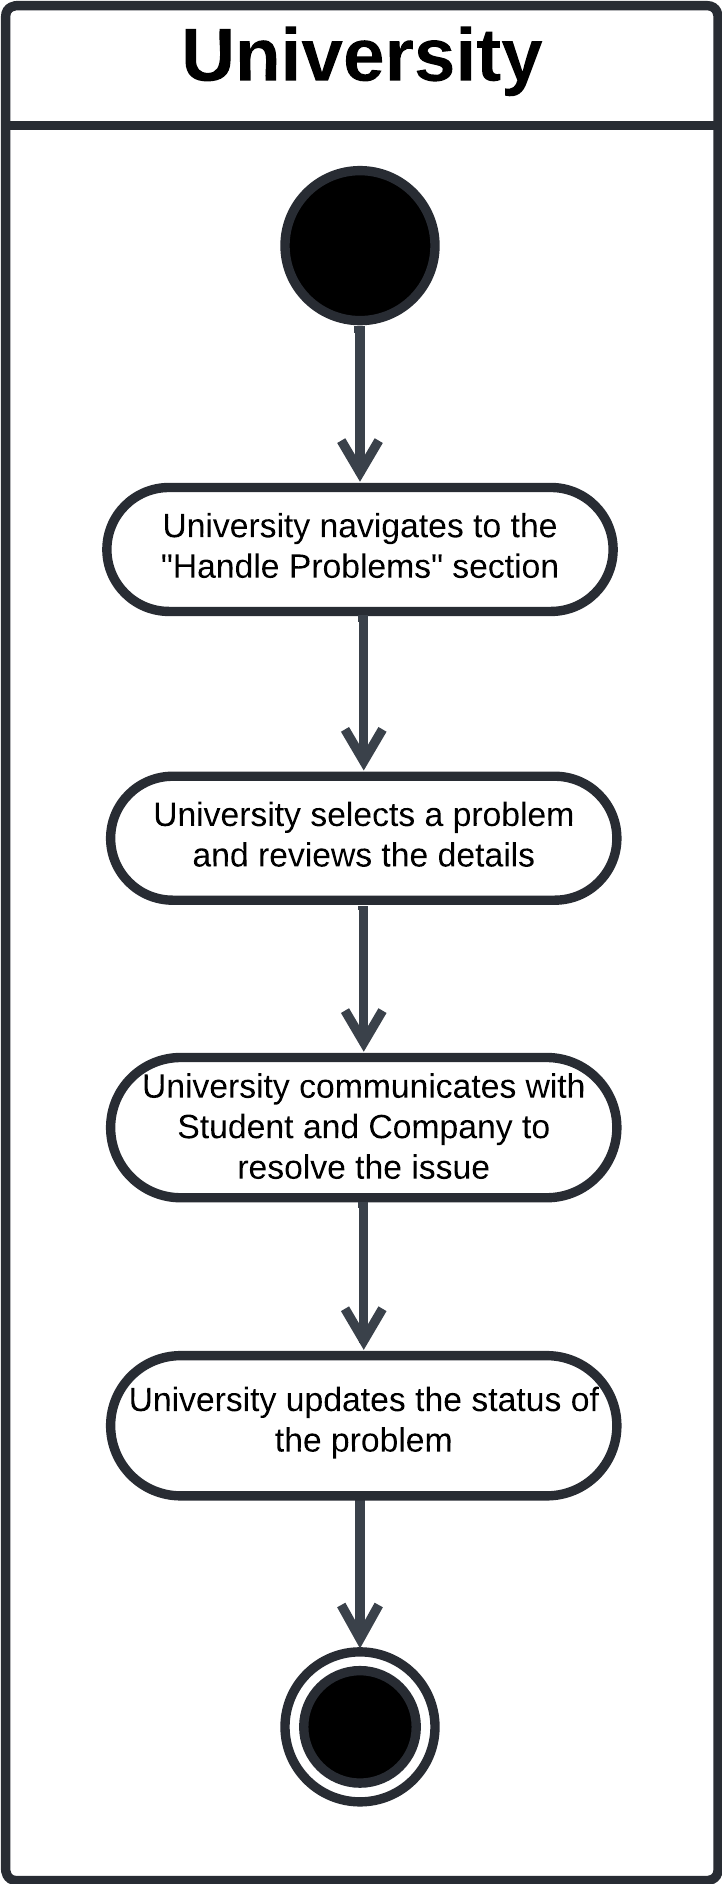
\includegraphics[width=0.65\linewidth]{LaTeXCode/images/activity diagram/UC17.png}
         \caption{Handle Problems during an Internship}
         \label{fig:handle_problems_ad}
     \end{center}
\end{figure}

\newpage

\subsubsection*{UC\cuc . Report Feedback after an Internship}
\begin{center}
    \begin{longtable}{|l|p{0.75\linewidth}|}
        \hline
        \textbf{Actor}            & Party (Student or Company) \\
        \hline
        \textbf{Entry Conditions} & The Party is logged into the S\&C platform and they have been actively involved in a finished internship. \\
        \hline
        \textbf{Flow of Events}       
        & \cucsteps. A non-mandatory survey appears in the Party's dashboard, asking to provide detailed information about the internship to feed the statistical analysis and improve the recommendation algorithm. \\ 
        & \cucsteps. The Party fills out the survey replying to each question. \\
        & \cucsteps. The Party submits the report by clicking the "Submit" button. \\ 
        \hline
        \textbf{Exit Conditions}   & The feedback provided by the Party is processed for improving the recommendation algorithm and recorded in the system. \\       
        \hline
        \textbf{Exceptions}       & \begin{itemize}
            \item The Party closes the survey without completing it: the system doesn't record any information and displays the Party's dashboard.
        \end{itemize} \\
        \hline
    \end{longtable}
\end{center}

\begin{figure}[H]
    \begin{center}
         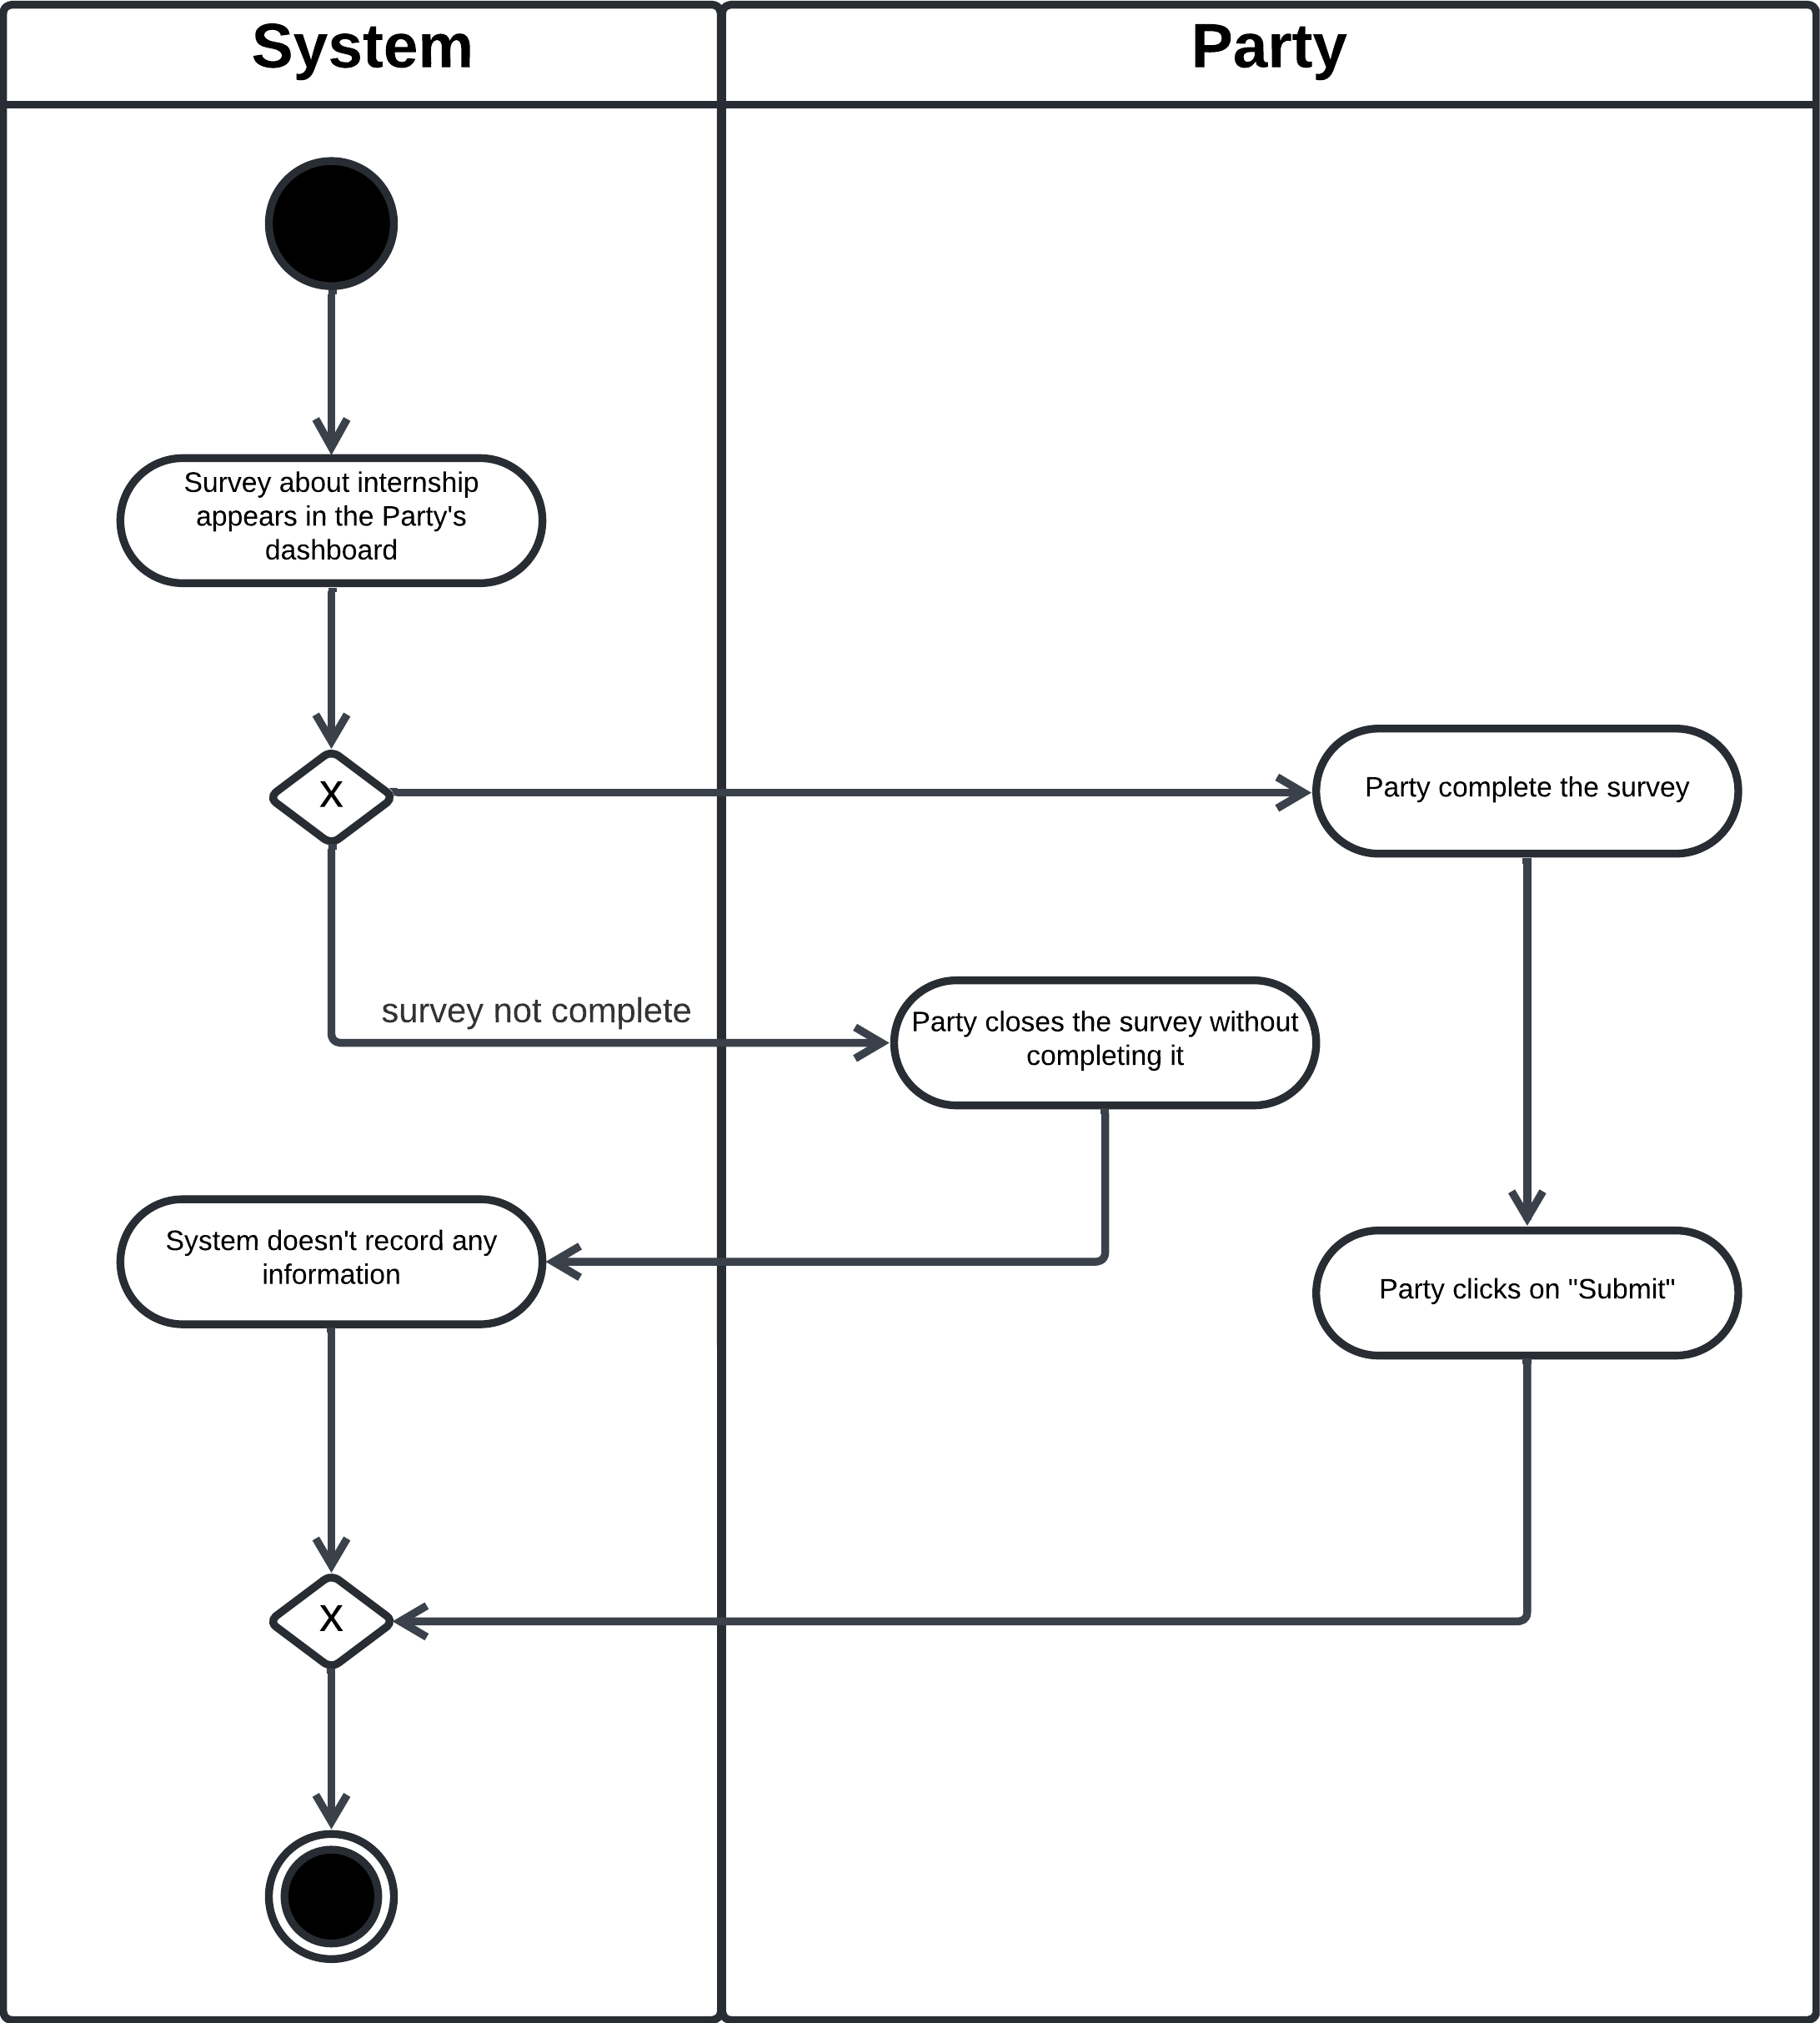
\includegraphics[width=1\linewidth]{LaTeXCode/images/activity diagram/UC18.png}
         \caption{Report Feedback after an Internship}
         \label{fig:report_problems_ad}
     \end{center}
\end{figure}

\newpage

\subsubsection*{UC\cuc . Suggest Optimizations for a Student Profile}
\begin{center}
    \begin{longtable}{|l|p{0.75\linewidth}|}
        \hline
        \textbf{Actor}            & Student\\
        \hline
        \textbf{Entry Conditions} & The Student is logged into the S\&C platform.\\
        \hline
        \textbf{Flow of Events}   
        & \cucsteps. In their "Profile" section, the Student clicks the "Improve Profile" button. \\ 
        & \cucsteps. The system automatically analyzes the student's profile, reviewing the following details:
        \begin{itemize}
            \item Academic background
            \item Skills
            \item Uploaded CV
            \item Certifications and extracurricular activities
        \end{itemize}\\
        & \cucsteps. Based on the analysis, the system generates a list of personalized suggestions to improve the profile which can belong to one of the following categories:
        \begin{itemize}
            \item Add additional skills or certifications.
            \item Update academic details or achievements.
            \item Include or enhance descriptions of projects.
            \item Enhance the overall style by improving clarity or content.
        \end{itemize}\\
        & \cucsteps. The Student reviews the suggestions and eventually decides which one to implement via the  \hyperref[subsec: update_profile_uc]{\uline{UC. Update User Profile}} functionality. \\
        \hline
        \textbf{Exit Conditions}   & The Student's profile is possibly optimized, improving its appeal and relevance for obtaining more internship offers in the future. \\       
        \hline
        \textbf{Exceptions}       & \begin{itemize}
            \item No optimizations can be found: the system doesn't provide any suggestions and terminates silently.
        \end{itemize}\\
        \hline
    \end{longtable}
\end{center}

\begin{figure}[H]
    \begin{center}
         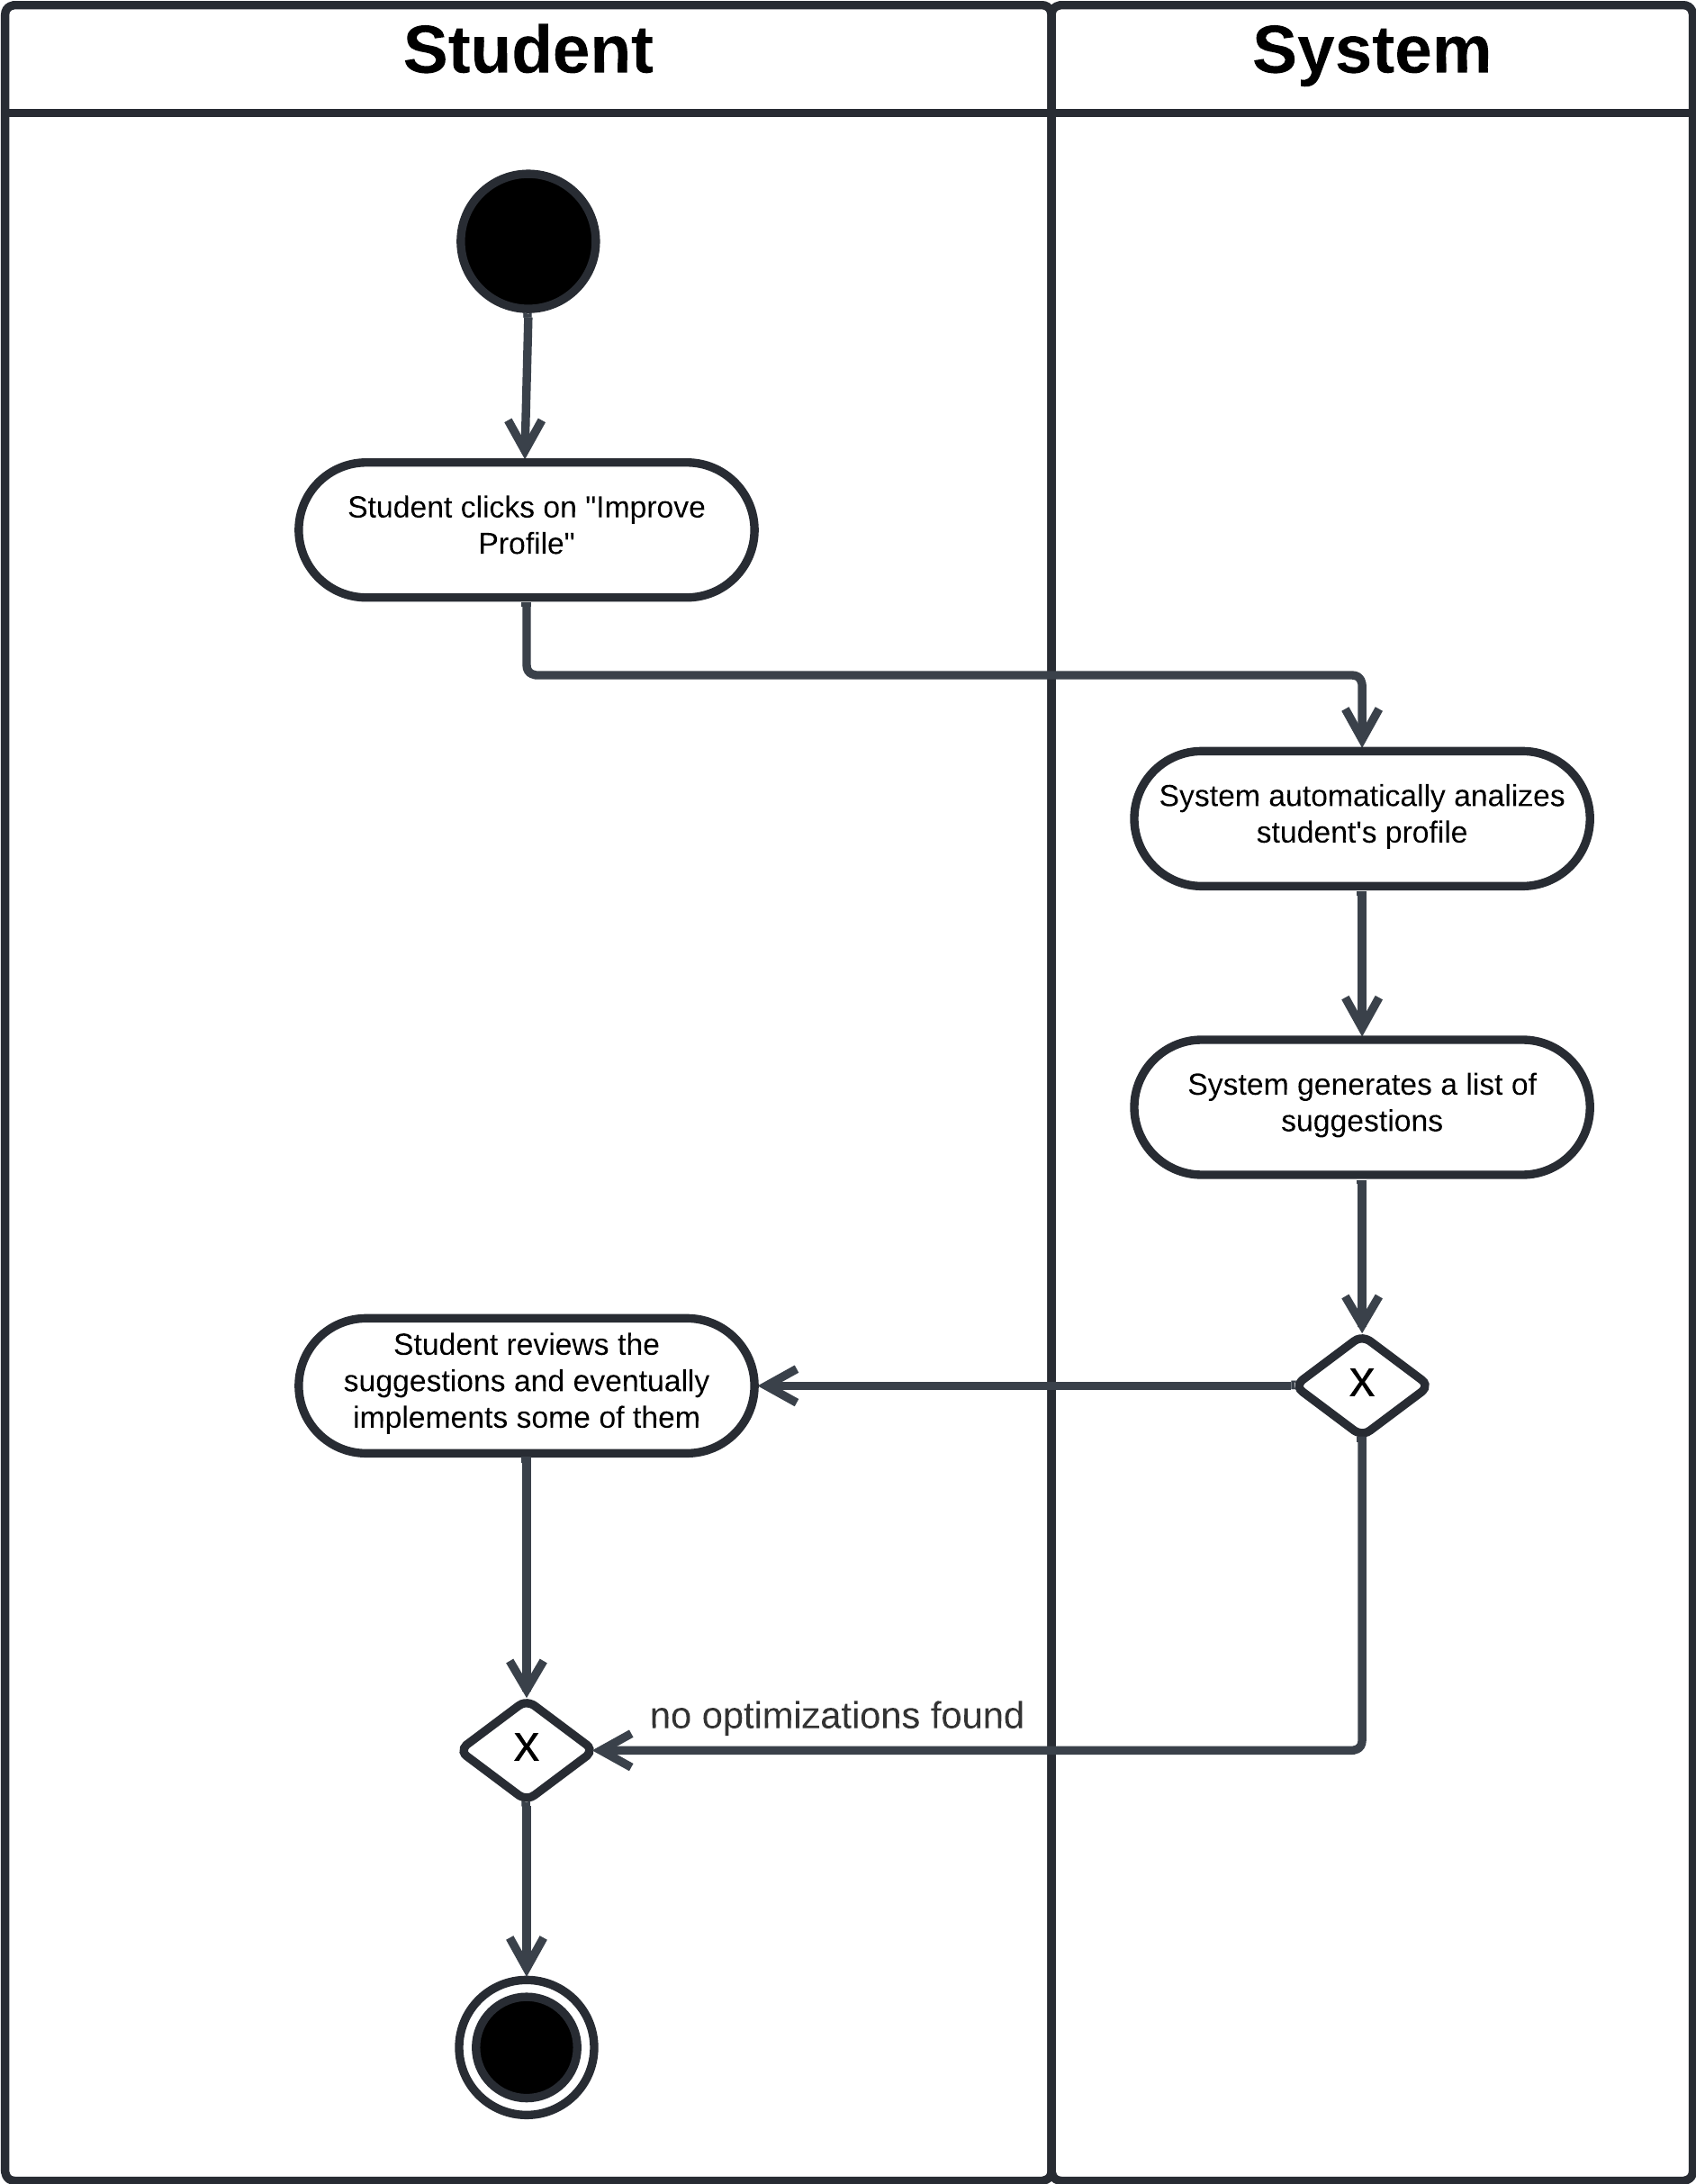
\includegraphics[width=1\linewidth]{LaTeXCode/images/activity diagram/UC19.png}
         \caption{Suggest Optimizations for a Student Profile}
         \label{fig:suggest_optimizations_student_ad}
     \end{center}
\end{figure}

\newpage

\subsubsection*{UC\cuc . Suggest Optimizations for an Internship Offer}
\begin{center}
    \begin{longtable}{|l|p{0.75\linewidth}|}
        \hline
        \textbf{Actor}            & Company \\
        \hline
        \textbf{Entry Conditions} & The Company is logged into the S\&C platform.\\
        \hline
        \textbf{Flow of Events}   
        & \cucsteps. In an internship offer's page, the Company clicks the \newline "Improve Offer" button. \\
        & \cucsteps. The system automatically analyzes the selected internship offer, reviewing the following details:
            \begin{itemize}
                \item Description of the internship
                \item Application domain
                 \item Required skills
            \end{itemize} \\
        & \cucsteps. Based on the analysis, the system generates a list of suggestions to improve the offer:
            \begin{itemize}
                \item Refine the description to better specify tasks and requirements.
                \item Improve the application domain by incorporating additional information or further elaborating on the details already provided."
                \item Introduce or modify the set of required skills.
                \item Enhance the overall style by improving clarity or content.
            \end{itemize} \\
        & \cucsteps. The Company reviews the suggestions and eventually decides which one to implement via the \hyperref[subsec: update_internship_offer_uc]{\uline{UC. Update Internship Offer}} functionality. \\
        \hline
        \textbf{Exit Conditions}   & The Company's selected internship offer is possibly optimized, making it more attractive to students and improving internship visibility for the future.\\       
        \hline
        \textbf{Exceptions}       & \begin{itemize}
            \item No optimizations can be found: the system doesn't provide any suggestions and terminates silently.
        \end{itemize}\\
        \hline
    \end{longtable}
\end{center}

\begin{figure}[H]
    \begin{center}
         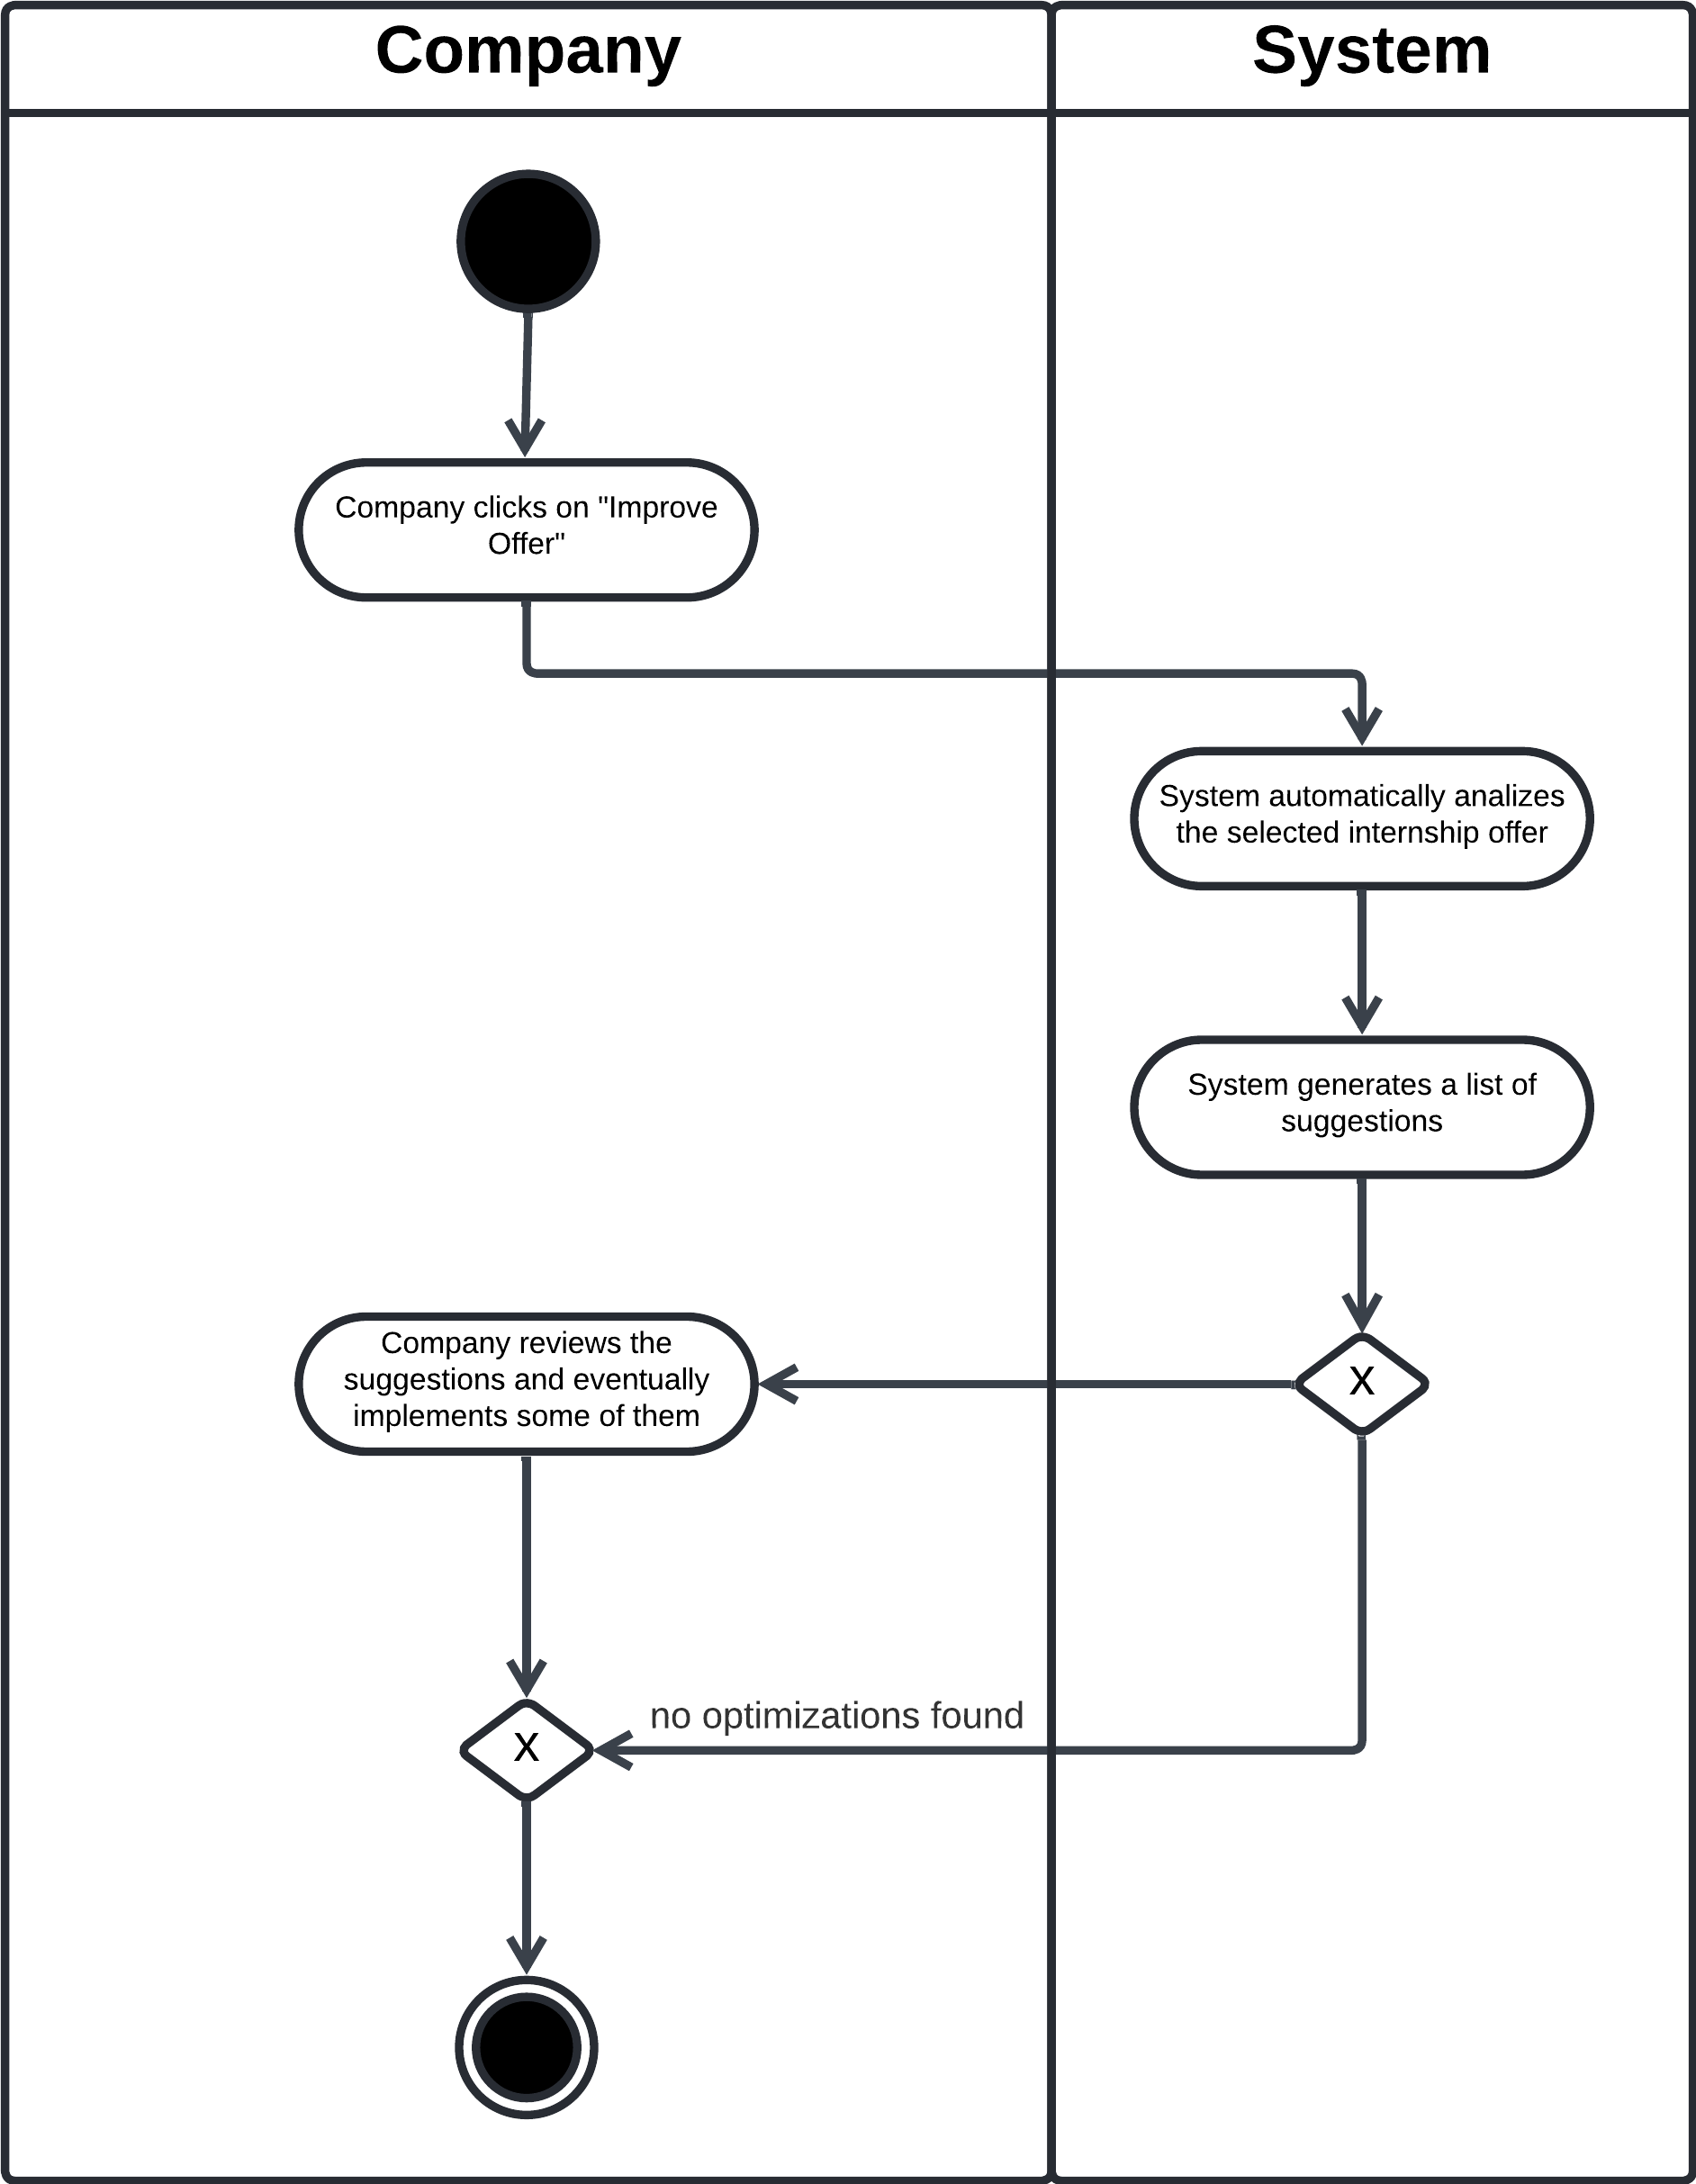
\includegraphics[width=1\linewidth]{LaTeXCode/images/activity diagram/UC20.png}
         \caption{Suggest Optimizations for an Internship Offer}
         \label{fig:suggest_optimizations_internship_ad}
     \end{center}
\end{figure}

\newpage

\subsection{Mapping On Requirements}
\label{subsec:mapping_on_requirements}

\newcounter{row}
\setcounter{row}{1}
\newcommand{\crow} {\therow\stepcounter{row}}

    \begin{longtable}{
        |>{\centering\arraybackslash}p{2cm}
        |>{\centering\arraybackslash}p{2cm}
        |>{\centering\arraybackslash}p{5cm}
        |>{\centering\arraybackslash}p{3.5cm}
        |>{\centering\arraybackslash}p{2cm}|
    }
        \hline
        \textbf{Row ID} & \textbf{Goal ID} & \textbf{Req ID} & \textbf{DA ID} & \textbf{UC ID} \\ \hline
        \endfirsthead
        \hline
        \textbf{Row ID} & \textbf{Goal ID} & \textbf{Req ID} & \textbf{DA ID} & \textbf{UC ID} \\ \hline
        \endhead
        \hline
        \endfoot
        \hline
        \endlastfoot
        \crow & G1 & R1, R2, R17 & DA1 to DA6 & UC1 \\ \hline
        \crow & G1 & R1, R2 & DA1 to DA6 & UC2 \\ \hline
        \crow & G1 & R1, R2 & DA1 to DA6 & UC3 \\ \hline
        \crow & G1 to G12 & R2 & DA1, DA7 & UC4 \\ \hline
        \crow & G1 & R3, R18 & DA1 to DA6 & UC5 \\ \hline
        \crow & G2 & R4, R5, R16 & DA1, DA7 & UC6 \\ \hline
        \crow & G2 & R2, R6, R7, R14, R15, R20, R21 & DA1, DA7 & UC7 \\ \hline
        \crow & G3 & R2, R8, R9 & DA1, DA8 & UC8 \\ \hline
        \crow & G3 & R2, R10, R11, R12, R13 & DA1, DA8 & UC9 \\ \hline
        \crow & G4, G5 & R2, R16, R17, R18, R19, R20, R24, R38 & DA1 & UC10 \\ \hline
        \crow & G4 & R2, R10, R11, R12, R13, R22, R23 & DA1 & UC11 \\ \hline
        \crow & G5 & R2, R16, R22, R24 & DA1 & UC12 \\ \hline
        \crow & G6 & R2, R25, R26, R27, R28, R29, R30, R31 & DA1, DA9, DA10 & UC13 \\ \hline
        \crow & G7 & R2, R32 & DA1, DA11 & UC14 \\ \hline
        \crow & G7 & R2, R33 & DA1, DA11 & UC15 \\ \hline
        \crow & G8 & R2, R34, R35 & DA1, DA12 & UC16 \\ \hline
        \crow & G9 & R2, R36 & DA1, DA13 & UC17 \\ \hline
        \crow & G10 & R2, R37, R38 & DA1, DA14 & UC18 \\ \hline
        \crow & G11 & R2, R39 & DA1 & UC19 \\ \hline
        \crow & G12 & R2, R40 & DA1 & UC20
    \label{tab:traceability}
    \end{longtable}

%We are linking to the UC only the Requirements which involve some concrete step of the UC.E.g. withdraw doesn't interact with UC Apply even if it discards applications

\section{Performance Requirements}
\label{sec:performance_requirements}

As the system does not supply any particular critical functionality to its users, it is acceptable if there are relatively small delays in the system's response times: therefore, constraints about the system's performance are in principle very lax/loose. On the other hand, requirements for the quality of the system are instead tight:

\begin{itemize}
    \item Anytime, the system shall be able to handle a load of up to 10000 concurrent Users without significant performance degradation: however, it shall also be scalable enough for this amount to be increased as a consequence of business decisions which cause the system's scope to widen.
    \item When generating recommendations, both accuracy and F1 score of the mechanisms employed for identifying those recommendations shall be at least 0.8. 
    \item Whenever receiving a request, the system shall respond to the requesting User in less than 5 seconds. This doesn't include recommendations generation, which, however, should be able to be carried out for up to 1.000.000.000 different users.
    \item Whenever any kind of information (including new recommendations, interview invites, or complaints) becomes available to a User, the system shall "append" it to that User's profile in the appropriate section within the following 0.01 seconds, so that it can immediately be shown to that User if they are logged in.
\end{itemize}

\section{Design Constraints}
\label{sec:design_constraints}%

\subsection{Standards Compliance}
\label{sec:standards_compliance}%

This system is designed to adhere to a range of standards and regulations to ensure compliance with legal, technical, and usability requirements. In the following, we outline the primary standards considered:

\begin{enumerate}
\item \textbf{General Data Protection Regulation (GDPR)}
The platform ensures compliance with GDPR to protect users’ personal data. Key measures include:
\begin{itemize}
    \item Data minimization and anonymization techniques for data storage.
    \item Mechanisms for users to access, modify, and delete their data.
    \item Transparent consent collection processes and data usage policies, ensuring that the user is aware on which operations and processes are applied to the shared data.
\end{itemize}
By integrating these security measures, the S\&C platform aims to foster user trust and compliance with current regulations.

\item \textbf{World Wide Web Consortium (W3C)}
The system adheres to W3C standards to ensure interoperability and usability across modern browsers. Some useful target objectives derived from the guidelines are:
\begin{itemize}
    \item Use meaningful HTML elements to structure content properly, enabling assistive technologies to interpret the page effectively.
    \item Follow WAI-ARIA (Web Accessibility Initiative–Accessible Rich Internet Applications) standard, a framework for adding attributes to identify features for user interaction, how they relate to each other, and their current state
    \item Perform decisions in order to reduce load times and enhance responsiveness.
\end{itemize}

\item \textbf{Web Content Accessibility Guidelines (WCAG)}
To ensure accessibility, the system follows the latest WCAG standards, a subset of W3C standard that outlines principles for making web content more accessible for people with disabilities:
\begin{itemize}
    \item Support for assistive technologies: screen readers and magnifiers, speech recognition software, keyboard-only navigation. The majority of the accessibility tools are already provided by the OS; the main focus should be in ensuring that such technologies are fully supported and working while interacting with the system.
    \item Accessible navigation structures and compatibility across various devices and input methods.
\end{itemize}
\end{enumerate}

\subsection{Hardware Limitations}
\label{sec:hardware_limitations}%
Considering the nature of the system, which is a WebApp, hardware limitations are minimal, as the system is designed to be lightweight and operates on standard devices and browsers, requiring only basic hardware specifications.

\section{Software System Attributes}
\label{sec:software_system_attributes}%

The main attributes that the system to be developed shall present are outlined here, listed in order of importance for its correct functioning.

\subsection{Reliability}
\label{sec:reliability}%

The system shall ensure high reliability: namely, it shall handle failures effectively and promptly recover from disruptions, minimizing total downtime, frequency of failures and number of functionalities involved. This shall be achieved by employing standard mechanisms for fault tolerance, such as replication of data storage or back-end computation nodes, ensuring no single point of failure compromises the system.

\subsection{Availability}
\label{sec:availability}%

The system shall guarantee at least a 2-nines availability (99\%, or a total downtime of at most 3.65 days/year), ensuring it is available except for planned maintenance, which should occur outside peak hours and be announced in advance anyway.
The decision is based on the fact that it does not offer any critical service to users that cannot be postponed in time.
A robust monitoring system shall track application health and trigger alerts for any performance issues or downtime.

\subsection{Security}
\label{sec:security}%

The system shall implement secure authentication and authorization mechanisms to verify user identities and restrict access to features based on user roles. Such guarantees may be implemented through strong password policies, 2FA, encrypted communication protocols (e.g., HTTPS), etc.
Additionally, the platform must ensure data integrity by preventing unauthorized modifications and preserving the accuracy of stored information, both physically and virtually.
To uphold confidentiality, the system shall encrypt sensitive data both in transit and at rest, ensuring that data remains unreadable even if intercepted or exposed. Secure data storage practices must be observed.
Moreover, the system must be resilient to common attack vectors, including SQL injection, cross-site scripting (XSS), and cross-site request forgery (CSRF). The platform should also incorporate regular security patches to address newly discovered vulnerabilities.

\subsection{Maintainability}
\label{sec:maintainability}%

System maintenance shall be planned for hardware or software upgrades, or for the deployment of production code containing additional functionalities, bug fixes or security updates. 
It should last 8 hours on average, theoretically enabling it to be carried out entirely outside peak traffic periods; in any case, it shall not exceed 24 hours. 
Maintenance bursts should happen exceptionally, possibly no more than twice or thrice a year, and shall always be announced in advance to the public (minimum 48 hours before). 
Software maintenance shall instead be employed right from the start of the development process by enforcing the application of best practices, in compliance with the industry standards; code shall be clean, modular, reusable, and low-coupled, to facilitate the introduction of new functionalities as needed.

\subsection{Portability}
\label{sec:portability}%

Since the platform is offered as a WebApp, it operates through standard web browsers and inherently supports compatibility across various operating systems.
Given this architecture, there is no need for native application installations, ensuring ease of use and minimizing setup complexity. Therefore, the chosen architecture and platform's reliance on web standards already solves all aspects related to portability.
The architecture of the platform shall be designed to offer portability, ensuring that it can be deployed across various environments and, eventually, hosting services. By utilizing containerization technologies, the application shall be easily migrated regardless of the underlying infrastructure.
